\documentclass{article}
\usepackage[a4paper, margin=1in]{geometry}
\usepackage{graphicx}
\usepackage{amsmath, amssymb, amsthm, float}
\usepackage{multirow}
\usepackage{comment}
\usepackage{xcolor}
\usepackage{booktabs}
\usepackage{hyperref}
\usepackage{subcaption}
\usepackage{float}
\hypersetup{
    %colorlinks=true, %set true if you want colored links
    %linktoc=all,     %set to all if you want both sections and subsections linked
    linkcolor=blue,  %choose some color if you want links to stand out
}

\newtheorem{theorem}{Theorem}
\theoremstyle{definition}
\newtheorem{definition}{Definition}

\newcommand{\addsouce}{\textsuperscript{\color{blue}[citation needed]}}
\newcommand{\todo}{{\color{blue}TODO: }}
\newcommand{\priority}{{\color{red}Priority: }}

%\setlength{\textheight}{24cm}
%\setlength{\textwidth}{160mm}
%\setlength{\topmargin}{-1.5cm}
%\setlength{\evensidemargin}{-0mm}
%\setlength{\oddsidemargin}{-0mm}

% Includes "References" in the Table of Contents
\usepackage[nottoc]{tocbibind}

\title{Report on Replication of ``Conformal prediction of option prices"}
\author{Miroslav Živanović, Naoaki Motobayashi, Oliver Löthgren}
\date{\today}

\begin{document}

\maketitle

\begin{abstract}
    This report documents the replication of~\cite{bastos}, where the Conformalized Quantile Regression (CQR)~\cite{cqr} is applied to estimate the prediction intervals of option prices. We follow the original methodology of~\cite{bastos} and identify critical shortcomings in its empirical coverage tests - mainly in terms of its failure to recognize the non-exchangeability of option prices when calibration and test sets are divided with respect to their temporal ordering. We fix these issues by testing coverage in a walk-forward, out-of-time scheme. We show that in an out-of-time testing, i.e. realistic applications of the CQR, coverage guarantees do not hold. 
    % Further, we also address the non-exchangeability of option price data by following~\cite{beyond_exchange}. The results indicate that ... TBA.
\end{abstract}

\tableofcontents

\section{Introduction}
When implementing a Machine Learning (ML) model, it is vital to validate its performance. In quantitative finance, where ML models tend to be point predictors, this is usually done by considering out-of-sample performance. Although this presents a correct methodology to test models, it only provides feedback on direct performance and foregoes the analysis of model uncertainty. Comparatively, confidence intervals and credible regions are prevalent in Classical and Bayesian Statistics, providing a framework for uncertainty quantification. These methods are either parametric, requiring distributional assumptions to be made, or nonparametric, which tends to make weaker distributional assumptions. Extending these concepts to estimate uncertainty intervals for ML models turns out to be more involved. Some of the most commonly used methods are Bayesian neural networks and deep ensembles as outlined in \cite{wutte}. However, BNNs impose distributional assumptions and are rarely used in practice due to their computational requirements. Deep ensembles are also a complicated methodology and both approaches do not have finite sample coverage guarantees. The ideal method of uncertainty quantification should be model agnostic and easily applied to any ML model, whilst also providing finite sample coverage.

Enter Conformal Prediction (CP): A versatile framework that can be applied to any ML model and provides uncertainty intervals with guaranteed coverage. It operates under a single core assumption, namely \textit{exchangeability} of data. Exchangeability is a form of symmetry assumption which essentially states that the order of training data does not matter. The methodology then constructs a prediction band based on empirical quantiles of model residuals, calculated by a symmetric scoring function such that these too are exchangeable, adjusted to achieve a certain coverage. It can of course be equivalently defined via its order statistics or its empirical cumulative distribution function (ECDF). For almost surely distinct values, it also provides a coverage upper bound. An important case of this is continuous models. Furthermore, coverage can be made exact by introducing auxiliary randomness, which transforms the discontinuous ECDF into a continuous one. The method is also modifiable by choice of an exogenous (negatively-oriented) conformity function, which may be selected to provide prediction bands adaptable to the input. CP intervals with coverage guarantees represent the uncertainty in the model's ability to accurately capture the phenomenon based on its training. The key being that it is based on the training data: if the target distribution changes the model will of course no longer be accurate. Inferences made from these intervals will therefore depend on ones confidence in the model. For example, in the case of a market-maker utilizing a state of the art ML pricing model, prices falling outside of the prediction band could indicate an arbitrage opportunity. On the other hand, an entity with less confidence in their models may perceive prices falling outside of predictions bands to indicate a deterioration in model performance, suggesting a need to recalibrate or tune the model. Nevertheless, there are remaining factors to be addressed. Firstly, whether the assumption of exchangeable data is valid, and secondly, to what extent conformal prediction is impacted if it is not. 

In this investigation, we consider the problem of option pricing as in \cite{bastos}, both replicating and extending these results. The underlying parameters of spot price, strike price, risk-free rate, implied volatility, and time to maturity are assumed to dictate an options value. The veracity of the exchangeability assumption in this application is questionable, so we expect coverage to be adversely affected. After presenting a brief summary of Conformal Prediction and its three main forms, Conformalized Quantile Regression is explored in a simulated setting where the exchangeability assumption can be both enforced and gradually relaxed. Discussing the validity of exchangeability in an option pricing setting and transitioning to an analysis using real data then explores CPs actual performance and associated effects on coverage. Applied performance of CP is further analyzed through the implementation of a more realistic forward testing scheme.



\section{Short Introduction to Conformal Predictions}

Conformal prediction provides a statistically rigorous framework for constructing prediction intervals with finite-sample coverage guarantees. It ensures that the intervals achieve a nominal coverage level for a predictive model, regardless of the underlying data distribution. This framework is model-agnostic and can be applied to any symmetric machine learning algorithm, making it a powerful tool for uncertainty quantification. Traditionally, conformal prediction assumes the notion of exchangeability to provide formal guarantees, but recent research has extended its applicability to non-exchangeable data.

\begin{definition}\label{def:exchangeability}
A sequence of random variables $(Z_1, Z_2, \dots, Z_n)$ is \textbf{exchangeable} if its joint distribution is invariant under any permutations $\pi$ of indices:
\begin{equation}\label{eq:exchangeability}
    P(Z_1, Z_2, \dots, Z_n) = P(Z_{\pi(1)}, Z_{\pi(2)}, \dots, Z_{\pi(n)}).
\end{equation}
\end{definition}
In addition to the exchangeability of data, algorithms for fitting the appropriate model are also assumed to yield results invariant under arbitrary permutations of data. This is formalized by the following definition, which will be used later in the formulation of Theorem \ref{th:full-conformal}.

\begin{definition}\label{def:symmetrical-algo}
Let a regression algorithm $\mathcal{A}$ be a mapping from a training data set of any size $n \geq 0$ to a regression function $\hat{\mu}$:
\[
\mathcal{A} : \bigcup_{n \geq 0} (\mathcal{X} \times \mathbb{R})^n \to \{\text{measurable functions } \hat{\mu} : \mathcal{X} \to \mathbb{R}\}.
\]
The algorithm $\mathcal{A}$ is said to treat the input data points \textbf{symmetrically} if its output is invariant under any permutation of data, i.e.,
\[
\mathcal{A}((x_{\pi(1)}, y_{\pi(1)}), \ldots, (x_{\pi(n)}, y_{\pi(n)})) = \mathcal{A}((x_1, y_1), \ldots, (x_n, y_n)),
\]
for all $n \geq 1$, all permutations $\pi$ on $[n] := \{1, \ldots, n\}$, and all $\{(x_i, y_i)\}_{i=1,\ldots,n}$.
\end{definition}

Conformal prediction generates prediction intervals $C(X_{n+1})$ for a new observation $Z_{n+1} = (X_{n+1}, Y_{n+1})$ to satisfy the desired coverage property:
\begin{equation} \label{eq:coverage}
    P(Y_{n+1} \in C(X_{n+1})) \geq 1 - \alpha,
\end{equation}
where $1 - \alpha$ is the nominal coverage level.

% Maybe we don't need the def of nonconformity score. That's something Vovk always mentions in details, but other ppl do not go into details in their papers. For example, use CQR paper or beyond exch. Do not even state a clear def of nonconformity score. They just say that the scoring function is symmetrical and whatever else (invariant under exch of data, or something like that). So maybe it is enough just to say that. For example, I looked at the new preprint of the book \cite{angelopoulos2024theoretical-foundations-cp}, and they don't even define nonconformity score, but they do discuss what kind of scoring function is used. See 3.2.1 The score function there. Here is the link to the book: https://arxiv.org/abs/2411.11824.

The methodology relies on nonconformity scores, given by a scoring function $s(x, y; \mathcal{D})$ that measures the atypicality of the model's evaluation $\hat{\mu}(x)$ of a data point $x$ relative to observed data $y$. Such a function represents model error and must be symmetric, meaning its output does not depend on the order of the data on which scores are computed, $\mathcal{D}$. Symmetry is required to ensure that the exchangeability of data is lifted to the exchangeability of nonconformity scores. Although coverage is guaranteed, the choice of scoring function dictates the shape and quality of prediction bands. For example, in regression tasks, a common choice of nonconformity score is the absolute residual:
\begin{equation} \label{eq:nonconformity}
    S_i = |Y_i - \hat{\mu}(X_i)|, \quad i = 1, \ldots, n,
\end{equation}
where $\hat{\mu}(X_i)$ is the predicted value for $Y_i$. This results in a prediction band of constant length for any input. Alternative nonconformity scores may be employed to better suit specific tasks. For instance,~\cite{cqr} proposes scores based on quantile regression, leading to tighter and adaptable prediction intervals in the presence of heteroskedasticity. Details are explained in Subsection \ref{subsec:cqr}.

In this report, we formulate conformal prediction in terms of a regression problem and employ the absolute residual in Equation~\eqref{eq:nonconformity}. Analogous conclusions hold for classification tasks, where prediction intervals $C(X_{n+1})$ are replaced by prediction sets $C(X_{n+1})$. We refer the reader to~\cite{gentle-intro} for an approachable introduction to conformal predictions. For a more rigorous yet still approachable introduction, we recommend the forthcoming~\cite{angelopoulos2024theoretical-foundations-cp}. The standard reference book is \cite{vovk2022algorithmic}.

\subsection{Full Conformal Prediction}
Full conformal prediction is the original formulation of the conformal prediction, and we state it here as the starting point for many theoretical results for other variants of conformal predictions. In the full conformal prediction framework, we have trained a model on a training set $\mathcal{D}_t$, containing data $Z_i = (X_i, Y_i)$ for $i=1, \dots, n$, and we are making a prediction at a test point $X_{n+1}$. To obtain prediction interval for the $\hat{Y}_{n+1}$, we firstly augment $\mathcal{D}_t$ by adding a synthetic point $Z_{n+1}^y = (X_{n+1}, y)$, where $y$ is the ``trial" or ``query" value, to get the augmented training set $\mathcal{D}$. Then, we refit the same model on $\mathcal{D}$. The nonconformity score for a particular trial value $y$ is given by
\begin{equation} \label{eq:full_conformal}
    S^y_i = 
    \begin{cases} 
    |Y_i - \hat{\mu}^y(X_i)|, & i = 1, \ldots, n, \\ % & i \leq n, \\
    |y - \hat{\mu}^y(X_{n+1})|, & i = n+1,
    \end{cases}
\end{equation}
where $\hat{\mu}^y$ is the predictive model trained on $(Z_1, \dots, Z_n, Z_{n+1}^y)$. The prediction interval is then
\begin{equation} \label{eq:full_prediction_set}
    \hat{C}(X_{n+1}) = \left\{y : S^y_{n+1} \leq Q\left(S^y_1, \dots, S^y_{n}\,; \, (1-\alpha)(n+1)/n\right)\right\}.
\end{equation}
where $Q(x_1, ..., x_n; p)$ stands for $p$th quantile of the nonconformity scores of data $x$. In practice, $\hat{C}(X_{n+1})$ is constructed by sweeping through a grid of trial values $y$. In essence, the trial value $Z_{n+1}^y$ is included in the augmented training to ensure exchangeability of all nonconformity scores $S_1, \dots, S_n, S_{n+1}^y$ given $\mathcal{D}$, and the prediction band $\hat{C}(X_{n+1})$ contains all values $y$ that lead to a score smaller than the $(1-\alpha)(n+1)/n$ quantile. Note that this set is the same whether the trial nonconformity $s(X_{n+1}, y; \mathcal{D}) = S_{n+1}^y$ is included in the quantile computation or not. This is because if $S_{n+1}^y < Q_n^y$, then $S_{n+1}^y \le Q_{n+1}^y$, and if $S_{n+1}^y = Q_{n}^y$, then $S_{n+1}^y = Q_{n+1}^y$, and of course $S_{n+1}^y > Q_{n}^y$ if and only if $S_{n+1}^y > Q_{n+1}^y$. The other way follows similarly. It is easier to see how this work by considering the equivalent formulation of the problem via order statistics, comparing the $\lceil(1-\alpha)(n+1)\rceil$ smallest values instead of quantiles.

\begin{theorem}\label{th:full-conformal}
Let a sequence of data points $(X_1, Y_1), \dots, (X_n, Y_n), (X_{n+1}, Y_{n+1})$ be exchangeable, and the algorithm $\mathcal{A}$ treats the input data points symmetrically. Then the full conformal prediction set defined in \eqref{eq:full_prediction_set} satisfies the following coverage guarantee
$$
\mathbb{P}\left\{ Y_{n+1} \in \widehat{C}_n(X_{n+1}) \right\} \geq 1 - \alpha % OR EVEN BETTER???: \in \left[ 1-\alpha , 1- \alpha + \frac{1}{n+1}\right)
$$
\end{theorem}
\begin{proof} This follows as exchangeable data with a symmetric scoring function will lead to exchangeable nonconformity scores. Including $S_{n+1}^y$ in the calculation of the quantile defining $\widehat{C}_n(X_{n+1})$ then implies the result as the rank of $S_{n+1}^y$ is distributed uniformly over $S_1, ..., S_{n+1}$ by exchangeability. See section 3.2 of \cite{angelopoulos2024theoretical-foundations-cp} for a rigorous proof of the theorem.

%\todo ADDED A CONCISE PROOF DETAILING STEPS AND REFERING TO MORE DETAILED ONE IN REFERENCE. %finish the proof if it is simple, or just find a precise reference (Oli or Miro), reference are %\cite{cqr, angelopoulos2024theoretical-foundations-cp, beyond_exchange, gentle-intro}
\end{proof}

Full conformal prediction often yields relatively tight intervals but is computationally expensive due to repeated model retraining. However, efficient implementations exist for specific models, such as ordinary least squares, kernel ridge regression~\cite{burnaev2014}, and the Lasso~\cite{lei2019}. 

\subsection{Split Conformal Prediction}

Split conformal prediction is computationally efficient but sacrifices some data for calibration, potentially reducing the predictive model's accuracy. Split conformal prediction, as formalized by~\cite{vovk2022algorithmic}, divides the data into two subsets: one for training the predictive model $\mathcal{D}_t$ and the other for calibration $\mathcal{D}$, taken to be of size $|\mathcal{D}| = n$. After training a model, the nonconformity scores are computed for the calibration set. The prediction interval for a new observation $X_{n+1}$ is then calculated as:
\begin{equation} \label{eq:split_conformal}
    C(X_{n+1}) = \left\{y : S_{n+1} = s(X_{n+1}, y) \le Q_{1-\alpha}\right\}
\end{equation}
where $Q_{1-\alpha}$ is the $(1-\alpha)(n+1)$-th quantile of  nonconformity scores $S_i = s(X_i, Y_i)$ from $\mathcal{D}$ for $i=1, ..., n$.

The same result as in \ref{th:full-conformal} holds for split conformal since split conformal can be viewed as a special case of full conformal. Here, a pre-fitted model $\hat{\mu}(X; \mathcal{D}_t)$ is used along with a new set of calibration data $\mathcal{D}$ disjoint from $\mathcal{D}_t$. In this setting, the scoring function is symmetric with respect to the calibration data because it is calculated from a model trained on $\mathcal{D}_t$ disjoint from $\mathcal{D}$. Thus, $s(x, y; \mathcal{D}_n) = f(\hat{\mu}(x; \mathcal{D}_t), y) = s(x, y)$, for some function $f$ lifting the argument from point $x$ to model output $\hat{\mu}(x; \mathcal{D}_t)$. Analogously to full conformal prediction, the prediction band is then given by $\hat{C}(X_{n+1}) = \left\{y : s(X_{n+1}, y) \le Q_{1-\alpha}\right\}$. Hence, it is equivalent to implementing full conformal prediction on a fixed pre-trained model, considering calibration data $\mathcal{D}$ as a new training set and $\mathcal{D} \cup (X_{n+1}, y)$ as the new augmented training set to both have no impact on the model.

Lengths of the prediction intervals produced by the full conformal have limited variability~\cite{Lei2016DistributionFreePI}, and for the split conformal PIs, they are all of the same width. This is an issue in applications where uncertainty varies greatly along the domain of covariates, and this is definitely the case in option pricing. For example, the uncertainty of option prices significantly varies across moneyness, as deep out-of-the-money and deep-in-the-money options are much less liquid, similarly for the very short time to maturity options.


\subsection{Conformalized Quantile Regression (CQR)}\label{subsec:cqr}

Instead of wrapping a point prediction model to obtain prediction intervals, we could train two quantile regression models to estimate directly the lower and upper quantiles, $q_{\alpha/2}(X)$ and $q_{1-\alpha/2}(X)$, of the conditional distribution of $Y$ given $X$. This approach, called \textbf{Conformalized Quantile Regression (CQR)}, was developed in~\cite{cqr}. The nonconformity score for CQR is:
\begin{equation} \label{eq:cqr_nonconformity}
    S_i = \max\left[q_{\alpha/2}(X_i) - Y_i, Y_i - q_{1-\alpha/2}(X_i)\right].
\end{equation}
where $X_i$, $i=1, ..., n$, are from the calibration set $\mathcal{D}_n$. The prediction interval for a new observation $X_{n+1}$ is:
\begin{equation} \label{eq:cqr_interval}
    C(X_{n+1}) = \left[q_{\alpha/2}(X_{n+1}) - Q_{1-\alpha}, q_{1-\alpha/2}(X_{n+1}) + Q_{1-\alpha}\right].
\end{equation}
where $Q_{1-\alpha}$ is
\begin{equation}
    Q\left(S_1, ..., S_n;\, (1-\alpha)(1+n)/n\right)
\end{equation}

The interpretation of this is that the plug in estimate prediction band $C(X_{n+1}) = [q_{\alpha/2}, q_{1-\alpha/2}]$ is adjusted to account for its miscoverage. CQR effectively captures local variability in the data, making it particularly useful in applications where uncertainty varies across the feature space, such as in option pricing~\cite{bastos}. In addition to being more adaptive than a classical split conformal or full conformal approach, CQR has also been shown to produce tighter prediction intervals and maintain coverage guarantees ~\cite{cqr}.

\begin{comment} WE WILL ADD THIS SUBSECTION ONLY IF IT IS USED IN THE REPORT
\subsection{Extensions for Non-exchangeable Data}
In practice, many datasets exhibit dependencies that violate the assumption of exchangeability. Recent extensions, such as weighted conformal prediction~\cite{beyond_exchange}, address these challenges by assigning weights to observations based on their relevance. For example, in a time-series setting, exponentially decaying weights, $w_i = \rho^{n+1-i}$, prioritize recent observations. The weighted prediction interval is:
\begin{equation} \label{eq:weighted_interval}
    C(X_{n+1}) = \hat{\mu}(X_{n+1}) \pm Q_{1-\alpha}\left(\sum_{i=1}^n w_i \delta_{S_i} + w_{n+1} \delta_{+\infty}\right),
\end{equation}
where $Q_{1-\alpha}$ is the weighted quantile of the nonconformity scores.
\end{comment}

\begin{comment} WE WILL ADD Mondrian ONLY IF IT IS USED IN THE REPORT
\subsection{Mondrian Conformal Prediction and Hierarchical Models}
\textit{Mondrian conformal prediction}, introduced by Vovk et al. (2005), partitions data into categories where exchangeability holds within each group. This approach is particularly useful in hierarchical models and applications involving group-specific distributions. For a dataset $(X_1, Y_1), \dots, (X_n, Y_n)$, a Mondrian taxonomy assigns categories:
\[
\kappa: Z \to K,
\]
and nonconformity scores are calculated within each category:
\[
S_i = |Y_i - \hat{\mu}(X_i)| \quad \text{if } \kappa(Z_i) = \kappa(Z_j).
\]
Mondrian conformal prediction ensures category-specific coverage:
\[
P(Y_{n+1} \in C(X_{n+1}) \mid \kappa(Z_{n+1}) = k) \geq 1 - \alpha.
\]
In hierarchical contexts, such as multi-level healthcare data, where observations are drawn from group-specific distributions, Dunn et al. (2022) proposed methods like \textit{CDF pooling} and \textit{repeated subsampling} to adapt conformal prediction to nested structures.
\end{comment}

\section{Experiments with Simulated Data}
In this part of the study, synthetic data were generated using Monte Carlo simulations to replicate the data simulation procedure outlined in the original paper~\cite{bastos}. The goal is to establish a controllable environment to inspect the empirical coverage of prediction intervals for different degrees of exchangeability of generated data. In fact, our empirical coverage check indicates that the original paper~\cite{bastos} implemented a random and shuffled data split into calibration and test data, which artificially ensures the exchangeability of the data and therefore produces a valid coverage of the prediction intervals. In this section, we describe how we generated data slightly more realistically and how it led to the violation of exchangeability and loss of coverage of conformal prediction intervals.

\subsection{Data Simulation} % DONE

As in~\cite{bastos}, we firstly make random draws of five covariates $(S, \sigma, \tau, r, K)$, consisting of the spot price $S$, the annualized volatility of the underlying asset $\sigma$, the time-to-maturity in years $\tau$, the annualized risk-free interest rate $r$, and the strike price $K$. This is done in two steps. Firstly, $(S, \sigma, \tau, r)$ are sampled from their respective distributions as shown in Table~\ref{tab:distributions}, \emph{independently} of each other. Secondly, for each tuple of  $(S, \sigma, \tau, r)$ we draw $\kappa$ samples of random variable $z \sim N(1, 0.1)$, and then we calculate strike prices as $K = \frac{S}{z}$. This produces a realistic table of option prices in the following sense: for a fixed underlying and time, there will be multiple options on the market with different strike prices but the same $S$ and $\sigma$ (according to Black-Scholes)\footnote{In reality, we would have multiple maturities (and thus multiple effective interest rates associated with that maturity) for each instance of ($S, \sigma$). This additional complexity is neglected in our simulation, as well as in~\cite{bastos}, since ``multiple strikes per option" is sufficient to introduce dependencies between different data samples and violate exchangeability.}.

This simulation procedure introduces a dependency between covariates, which manifests as groups of $\kappa$ points in the dataset with $(S, \sigma, \tau, r)$ but different values of $K$. %Since each group of $\kappa$ points is associated with a fixed timestamp\footnote{We do not have a ``time'' variable in the simulation procedure, but implicitly, fixed $(S, \sigma, \tau, r)$ is associated with a fixed underlying, fixed time to maturity and fixed moment in time.}, and since in practice we would like to compute PIs for future timesteps (not the data which is already observed), the calibration/test split should respect this time constrain. In the case of our synthetic data, each group of $\kappa$ points should be part of either of the sets (proper training, calibration, validation, or test set).
In practice, a group of points with identical $(S, \sigma, \tau, r)$ appears 

Since each group of points is associated with a fixed timestamp\footnote{We do not have a ``time'' variable in the simulation procedure, but implicitly, fixed $(S, \sigma, \tau, r)$ is associated with a fixed underlying, fixed time to maturity and fixed moment in time.}, and since in practice we would like to compute PIs for future timesteps (not the data which is already observed), the calibration/test split should respect this time constraint. In the case of our synthetic data, each group of $\kappa$ points should be part of either of the sets (proper training, calibration, validation, or test set).

%\todo MIROSLAV: The argument of timestamps is invalid here - the current date is not included in the analysis. [Miroslav: you are correct, there is no notion of time in our simulation setup in an explicit form, but since in practice you want to compute PI for options at some timestamp in the future, you will not have points with identical $(S, \sigma, \tau, r)$ in both test and calibration set. Multiple identical $(S, \sigma, \tau, r)$ in practice appear only when you fix a timestamp, fix underlying and fix tau. Randomization between sets introduces exchangeability in an artificial way, and I that's what I tried to explain below] The only important part relating to time is the time to maturity, so we are not predicting "in the future", we are just learning the pricing function. We could input the data in any order to our ML algorithm and it would learn the same pricing function. But the issue and REASON WHY EXCHANGEABILITY IS RUINED is purely the fact that there are several strike prices with identical parameters, and reordering the data does not work with necessarily identical parameters [correct, learning is invariant under permutatins inside the training set; also, computation of nonconformity scores is invariant under permutations inside calibration set; same for permutations within the test set - which are all required by the requirement from \ref{th:full-conformal} that ``algorithm A treats the input data points symmetrically". What you are missing here is that we additionally need invariance under permutations of points between the test and calibration sets. This is what we do not have, but we artificially create it by having points with the same $(S, \sigma, \tau, r)$ in test and calibration, ie. by random splitting into test, train, calib.] It is not tied to splitting training and calibration sets. (Consider the case where you have options at the same time, but reorder the data for your different stocks to mix their options with different strike prices: this still ruins exchangeability) 

%Further question that is maybe irrelevant but interesting: Is there a way that we can get exchangeability of non-conformity scores (errors in pricing) despite the non-exchangeability of the data? This would mean that we can still apply conformal prediction  - I think one way to do this would be to standardize the 'spread' of strike prices around the spot and do the multi-price prediction we discussed in a meeting [I don't get the idea at the moment, but we can discuss it after the submission of the report] (END TODO)

The presence of data points with identical parameters but different strikes makes data non-exchangeable, and unfortunately, the original paper~\cite{bastos} does not address this issue. To see why dependency makes data non-exchangeable, consider the following example. Let $\kappa=2$, and let us have two timestamps labeled with $t_1$ and $t_2$, making the full dataset be:
$$
(Z_1, Z_2, Z_3, Z_4) \equiv (Z_{t_1, 1},Z_{t_1, 2},Z_{t_2, 1},Z_{t_2, 2})
$$
where $(Z_{t_1, 1}, Z_{t_1, 2})$ are samples for the same timestamp on the same underlying so that both samples will have identical values of $(S, \sigma, \tau, r)$ but different values of $K$. An analogous statement holds for the $(Z_{t_2, 1}, Z_{t_2, 2})$ samples. It is easy to see that splitting data into the calibration set and test set as $\mathcal{S}_{calib.} = (Z_{t_1, 1}, Z_{t_1, 2})$ and $\mathcal{S}_{test} = \{Z_{t_2, 1}\}$ makes for a non-exchangeable sequence of $(Z_1, Z_2, Z_3) \equiv (Z_{t_1, 1}, Z_{t_1, 2}, Z_{t_2, 1})$. Indeed, the joint distribution of $(Z_{t_1, 1}, Z_{t_1, 2}, Z_{t_2, 1})$ will have to output identical values of $(S, \sigma, \tau, r)$ for the first two variables, where any non-identity permutation of these three variables will require either the second and the third or the first and the third variable of the sequence to have identical values of $(S, \sigma, \tau, r)$, which violates \eqref{eq:exchangeability}.

On the other hand, if we split data into the test and calibration \emph{randomly}, which means by randomly drawing a permutation $\tilde \pi$ from the group of permutations of a three-element sequence and $\mathcal{S}_{calib.} = (Z_{\tilde{\pi}(1)}, Z_{\tilde{\pi}(2)})$ and $\mathcal{S}_{test} = \{Z_{\tilde{\pi}(3)}\}$; and then apply $\pi$ permutation from \eqref{eq:exchangeability}, the exchangeability condition reads:
\begin{equation}\label{eq:pi-tilde-pi}
    P(Z_{\tilde{\pi}(1)},Z_{\tilde{\pi}(2)}, Z_{\tilde{\pi}(3)}) = P(Z_{\pi(\tilde{\pi}(1))},Z_{\pi(\tilde{\pi}(2))}, Z_{\pi(\tilde{\pi}(3))}), \qquad \forall \pi
\end{equation}
where $P$ also includes probability of drawing $\tilde \pi$ from the permutation group. If the drawing of any $\tilde \pi$ from the permutation group is equally likely, then 
$$
(\tilde{\pi}(1), \tilde{\pi}(2), \tilde{\pi}(3)) \overset{d}{=}  (\pi\tilde{\pi}(1), \pi\tilde{\pi}(2), \pi\tilde{\pi}(3)), \qquad \forall \pi
$$
because $\pi\tilde{\pi}$ is also a permutation, and drawing $\pi\tilde{\pi}$ from the group is equally likely as drawing $\tilde{\pi}$. Since drawing of $\tilde{\pi}$, and equivalently the drawing of $\pi\tilde{\pi}$, is independent of $(Z_1, Z_2, Z_3)$, equality in \eqref{eq:pi-tilde-pi} holds.

%$$
%P(Z_{\tilde{\pi}(1)},Z_{\tilde{\pi}(2)}, Z_{\tilde{\pi}(3)}) = P(Z_{\hat{\pi}(1)},Z_{\hat{\pi}(2)}, %Z_{\hat{\pi}(3)}|\hat{\pi} = \tilde{\pi}) P(\hat{\pi})
%$$, and exchangeability of $(Z_{\tilde{\pi}(1)},Z_{\tilde{\pi}(2)}, Z_{\tilde{\pi}(3)})$, with respect to %permutation $\pi$ holds. The reasoning is applicable for more than three variables.

The ``repetition" of $(S, \sigma, \tau, r)$ among the sample points violates exchangeability in our simulation setup, so the basic intuition tells us that we expect more non-exchangeable data as we increase the $\kappa / n$ ratio and vice versa. Methodology in~\cite{bastos} draws $\kappa=4$ distinct strike prices. We extend the analysis by additional simulations with $\kappa=1$ (i.e., exchangeable data) and $\kappa=20$ configurations. These configurations allowed us to check the sensitivity of exchangeability, and consequently empirical coverage, to changes in $\kappa / n$.

\begin{table}[]
\centering
\caption{Distributions for Simulated Variables. $U(a, b)$ represents the uniform distribution over $[a, b]$, while $N(\mu, \sigma^2)$ denotes the normal distribution with mean $\mu$ and variance $\sigma^2$.}
\label{tab:distributions}
\begin{tabular}{@{}ll@{}}
\toprule
\textbf{Variable} & \textbf{Distribution} \\
\midrule
Spot Price ($S$) & $S \sim U(500, 1500)$ \\
Volatility ($\sigma$) & $\sigma \sim U(0.1, 1)$ \\
Time-to-Maturity ($\tau$) & $\tau \sim U\left(\frac{14}{252}, 2\right)$ \\
Risk-Free Rate ($r$) & $r \sim U(0.001, 0.05)$ \\
Strike Price ($K$) & $K = \frac{S}{z}, \, z \sim N(1, 0.1)$ \\
% variance of 0.1 => std=sqrt(0.1)=0.316
% ~300 strikes will be negative
% The author probably used 0.1 as a std, not variance.
% With std=0.1, the number of negative strikes will be ~0
% That was a bad decision by me (Miroslav) because it only made less than 0.1% of prices negative,
% which we could have just manually changed sign to positive. Too late now.
\bottomrule
\end{tabular}
\end{table} 

To generate values of the dependent variable, i.e. option prices, we first have to decide on the type of exercise (European, American, etc.) and payout (call or put). Data for American options are more available, so to make simulation experiments comparable with the experiments with real data, the~\cite{bastos} focuses only on generating data for American options. This is an involving process for the general case, but in the special case of zero dividend payouts and American call option, as early exercise provides no additional value and the price matches that of an European call option. We follow the same decision as in~\cite{bastos} and use the Black-Scholes formula to price the options. 

Given the property of homogeneity of degree one of the Black-Scholes formula with respect to spot and strike prices, all prices were normalized by the strike price $K$. The resulting input-output pairs for the machine learning models were structured as:
\begin{equation}
\label{eq:inputs}
\text{Inputs: } \left\{ \frac{S}{K}, \sigma, \tau, r \right\}, \quad \text{Target: } \frac{V_{\text{BS}}}{K}.
\end{equation}

Datasets of varying sizes were created to test the impact of sample size on the performance of conformal prediction. Specifically, datasets of $20,000$, $50,000$, $100,000$, and $200,000$ observations were generated to replicate the results from the original study. Additionally, smaller datasets with $5,000$ and $10,000$ observations were included to inspect better the dependence of empirical coverage on $\kappa / n$.

For CQR, the dataset was split into ``proper" training, calibration, and validation subsets by taking $60\%$, $20\%$, $20\%$ of the original data set, respectively, and this splitting is done \emph{randomly}. For \textbf{Non-Conformal Quantile Regression (NQR)}, which is just the usual quantile regression algorithm without postprocessing techniques on PIs, the training set consisted of $80\%$ of the data, with the remaining $20\%$ used for validation. Independently from these sets, we generate a test sample of 500.000 points, in line with the discussion from this subsection. It means that no ``repetitions" of $(S, \sigma, \tau, r)$ are present in the calibration and test sets. Notebook \texttt{1.0-mz-simulate-data.ipynb} documents the simulation process and some basic checks to ensure the simulation is correctly implemented.

\subsection{Gradient Boosting Machines as CQR, and Hyperparameter Tuning}
This subsection follows the summary given in the original paper~\cite{bastos}. Starting with the foundational contributions by~\cite{hutchinson1994, malliaris1993}, machine learning has been extensively applied to option pricing and hedging. Feed-forward neural networks have been widely adopted for option pricing~\cite{anders1998, andreou2010, garcia2000}. However, comparisons by~\cite{ivascu2021} have demonstrated that tree-based ensemble methods, including random forests and gradient boosting machines, frequently outperform neural networks in pricing options. These findings are supported by more general research suggesting that tree-based models excel on tabular data due to their ability to handle nonlinear relationships and heterogeneous features~\cite{grinsztajn2022}.

In this study, we implement the Light Gradient Boosting Machine (LightGBM) algorithm, proposed by~\cite{ke2017}, as the primary regression model for CQR, following the procedure in the original work by~\cite{bastos}. LightGBM constructs an ensemble of decision trees to approximate the relationship between the input features and the response variable. The prediction, $\hat{Y}$, is expressed as:
\begin{equation}
\hat{Y} = \sum_{k=1}^K f_k(X),
\end{equation}
where $f_k(X)$ represents the output of the $k$-th decision tree, with $X$ being the input feature vector $\{\frac{S}{K}, \sigma, \tau, r\}$. The training process iteratively minimizes a predefined loss function by adding new trees to the ensemble to correct residual errors of the previous steps.

For quantile regression, LightGBM minimizes the pinball loss function:
\begin{equation}
\mathcal{L}(Y, \hat{Y}) =
\begin{cases}
\alpha \left(Y - \hat{Y}\right), & \text{if } Y \geq \hat{Y}, \\
(1-\alpha) \left(\hat{Y} - Y\right), & \text{if } Y < \hat{Y},
\end{cases}
\end{equation}
where $\alpha$ corresponds to the quantile being predicted, $Y$ is the actual normalized price $\frac{C_{\text{BS}}}{K}$, and $\hat{Y}$ is the predicted quantile. This loss function enables the model to estimate the lower and upper quantiles, $\hat{q}_{\alpha/2}(X)$ and $\hat{q}_{1-\alpha/2}(X)$, respectively, in order to construct prediction intervals in CQR~\cite{cqr}.

A grid search was performed to identify the optimal hyperparameters for each dataset. The hyperparameter search space is shown in Table~\ref{tab:hyperparameters}:

\begin{table}[]
\centering
\caption{Hyperparameter Search Space for LightGBM}
\label{tab:hyperparameters}
\begin{tabular}{@{}ll@{}}
\toprule
\textbf{Hyperparameter}         & \textbf{Values}            \\ \midrule
Number of Trees ($K$)         & \{100, 500, 1000, 2500, 5000\} \\
Maximum Depth ($d$)           & \{8, 16, 32, 64\}          \\
Maximum Leaves per Tree ($l_{\max}$) & \{32, 64, 128, 256\}   \\
Learning Rate ($\eta$)        & \{0.005, 0.01, 0.05, 0.1, 0.5\} \\ \bottomrule
\end{tabular}
\end{table}

Each hyperparameter combination was evaluated by training a model in the training set and validating it on the validation set. The objective function minimized during the search was the mean absolute error (MAE), which is equivalent to the pinball loss with $\alpha=0.5$ (estimation of the median):
\begin{equation}
\label{eq:mae}
\text{MAE} = \frac{1}{n_{\text{val}}} \sum_{i \in \mathcal{I}_{\text{val}}} \left| Y_i - \hat{Y}_i \right|,
\end{equation}
where $n_{\text{val}}$ is the number of validation samples, and $\mathcal{I}_{\text{val}}$ represents the indices of the validation data. For each sample, the hyperparameter configuration that yielded the lowest MAE was selected as optimal.

The LightGBM model was trained on the dataset defined in Eq.~\eqref{eq:inputs}. For a new observation $X_{\text{test}}$, LightGBM predicted the conditional quantiles:
\begin{equation}
\hat{q}_{\alpha/2}(X) \quad \text{and} \quad \hat{q}_{1-\alpha/2}(X).
\end{equation}
For downstream applications, these predictions would be scaled back to monetary units using the strike price:
\begin{equation}
\hat{C}_{\text{BS, lower}} = K \cdot \hat{q}_{\alpha/2}(X_{\text{test}}), \quad \hat{C}_{\text{BS, upper}} = K \cdot \hat{q}_{1-\alpha/2}(X_{\text{test}}).
\end{equation}
The resulting intervals $[\hat{C}_{\text{BS, lower}}, \hat{C}_{\text{BS, upper}}]$ formed the basis for conformal prediction.

In the notebook \texttt{2.0-mz-hp-optim-sim.ipynb} we document hyperparameter optimization.

\subsection{Empirical Coverage}

In order to evaluate the robustness of CQR and NQR, we analyze their ability to construct valid prediction intervals across datasets of varying sizes. This evaluation is performed in terms of two key metrics: \textbf{marginal coverage}, which measures the overall reliability of prediction intervals without conditioning on specific features, and \textbf{conditional coverage}, which assesses interval reliability within specific regions of the feature space. In our study, the input features correspond to the input features: moneyness, volatility, time-to-maturity, and interest rate.

\subsubsection{Marginal Coverage} % marginal means unconditional

\begin{definition}
\textbf{Marginal coverage} provides an unconditioned, global measure of the proportion of true responses that lie within the prediction intervals, averaged across the entire test set:
\begin{equation}
\text{Marginal Coverage} = \frac{1}{n_{\text{test}}} \sum_{i \in I_{\text{test}}} \mathbf{1}(Y_i \in C(X_i)),
\end{equation}
where $n_{\text{test}}$ is the number of test samples, $C(X_i)$ is the prediction interval for the input $X_i$, and $\mathbf{1}(Y_i \in C(X_i))$ is the indicator function, which equals $1$ if $Y_i$ lies within $C(X_i)$ and $0$ otherwise.
\end{definition}

Tables~\ref{tab:conformal-sim-res} and~\ref{tab:non-conformal-sim-res} summarize the marginal coverage achieved by CQR and NQR across varying training sample sizes and different values of $\kappa$, the number of strikes for each combination of $(S, r, \sigma, \tau)$ generated during simulation. For all experiments, the test sample size is fixed at $n_{\text{test}} = 500,000$.

In this discussion, we specifically focus on the results for $\kappa = 1$. For CQR, marginal coverage consistently improves as the training sample size increases, with values exceeding $90\%$ in most cases. For instance, a rate of $90.6\%$ is observed at $n_{\text{train}} = 10,000$, demonstrating the finite-sample coverage guarantees of CQR. In contrast, NQR shows radically lower marginal coverage, reaching only $74.6\%$ even with the largest training sample size of $n_{\text{train}} = 200,000$. These gap underscore the robustness of CQR in producing reliable prediction intervals, while emphasizing the limitations of NQR.

The parameter $\kappa$, which determines the number of strikes generated per unique $(S, \sigma, \tau, r)$ combination, poses significant challenges due to the potential non-exchangeability of the data. Larger $\kappa$ values induce dependencies that violate the exchangeability assumption, which are necessary for the theoretical validity of CQR and NQR. In particular, the simulation procedure in~\cite{bastos}, where $\kappa = 4$, inherently introduces such correlations. In fact, marginal coverage decreases significantly for both methods as $\kappa$ increases, casting doubt on their reliability in financial modeling contexts. This observation raises a fundamental question: Is option price data really exchangeable in practice? If not, the theoretical guarantees of prediction intervals under this assumption may not hold, prompting the need for caution and a reconsideration of modeling assumptions when applying these methods to real-world data, where exchangeability is rarely guaranteed.

% Results of the CQR
\begin{table}[H]
\centering
\caption{Coverage and the percentage of ill-conditioned outputs of \textbf{CQR}, in three simulation setups differing by the number $\kappa$ - the number of strikes generated per fixed $\{S,r,\sigma,\tau\}$. The sample size $n_{\text{train}}$ increases row-wise. The ill-ordered PI is the one for which the predicted lower bound ($lb$) is larger than the upper bound ($ub$). The ill-order PI and point prediction (PP) are those where $lb\leq pp \leq ub$ does not hold.}
\label{tab:conformal-sim-res}
\begin{tabular}{cl|lll|lll|lll}
\multicolumn{1}{l}{}                              &      & \multicolumn{3}{c|}{Coverage} & \multicolumn{3}{c|}{Ill ordered PI [\%]} & \multicolumn{3}{c}{Ill ord. PI and PP [\%]} \\ \hline
\multicolumn{1}{l}{}  & \ $\kappa \rightarrow$ & 1     & 4     & 20    & 1    & 4    & 20   & 1     & 4     & 20    \\ \hline
\multicolumn{1}{c|}{\multirow{6}{*}{\rotatebox{90}{$n_{\text{train}}$}}} & 5000 & 0.897   & 0.885   & 0.645  & 1.3     & 1.25    & 9.04    & 19.9      & 22.48     & 46.11     \\
\multicolumn{1}{c|}{} & 10000     & 0.906 & 0.879 & 0.678 & 1.15 & 1.78 & 9.42 & 18.91 & 24.01 & 44.68 \\
\multicolumn{1}{c|}{} & 20000     & 0.912 & 0.883 & 0.749 & 1.14 & 1.75 & 5.7  & 20.3  & 24    & 40.97 \\
\multicolumn{1}{c|}{} & 50000     & 0.906 & 0.887 & 0.782 & 0.88 & 1.04 & 4.37 & 21.26 & 24.91 & 37.11 \\
\multicolumn{1}{c|}{} & 100000    & 0.909 & 0.892 & 0.808 & 0.64 & 0.81 & 2.89 & 20.07 & 22.43 & 33.55 \\
\multicolumn{1}{c|}{} & 200000    & 0.902 & 0.887 & 0.795 & 0.26 & 0.36 & 1.96 & 22.61 & 24.67 & 34.89 \\ \hline
\end{tabular}
\end{table}

% Results of Non-Conformal QR
\begin{table}[H]
\centering
\caption{Coverage and the percentage of ill-conditioned outputs of \textbf{NQR}, in three simulation setups differing by the number $\kappa$ - the number of strikes generated per fixed $\{S,r,\sigma,\tau\}$. The sample size $n_{\text{train}}$ increases row-wise. The ill-ordered PI is the one for which the predicted lower bound ($lb$) is larger than the upper bound ($ub$). The ill-order PI and point prediction (PP) are those where $lb\leq pp \leq ub$ does not hold.}
\label{tab:non-conformal-sim-res}
\begin{tabular}{cl|lll|lll|lll}
\multicolumn{1}{l}{}                              &      & \multicolumn{3}{c|}{Coverage} & \multicolumn{3}{c|}{Ill ordered PI [\%]} & \multicolumn{3}{c}{Ill ord. PI and PP [\%]} \\ \hline
\multicolumn{1}{l}{}  & $\kappa \rightarrow$ & 1     & 4     & 20    & 1     & 4     & 20    & 1     & 4     & 20    \\ \hline
\multicolumn{1}{c|}{\multirow{6}{*}{\rotatebox{90}{$n_{\text{train}}$}}} & 5000 & 0.644   & 0.616   & 0.461  & 18.84    & 20    & 29.25    & 58.09     & 59.07     & 69.85     \\
\multicolumn{1}{c|}{} & 10000     & 0.663 & 0.629 & 0.55  & 17.28 & 21.14 & 31.18 & 57.62 & 60.68 & 69.15 \\
\multicolumn{1}{c|}{} & 20000     & 0.674 & 0.643 & 0.567 & 14.1  & 16.53 & 24.96 & 53.74 & 56.77 & 66.45 \\
\multicolumn{1}{c|}{} & 50000     & 0.702 & 0.686 & 0.616 & 8.63  & 9.57  & 16.25 & 48.82 & 49.64 & 57.31 \\
\multicolumn{1}{c|}{} & 100000    & 0.719 & 0.703 & 0.647 & 6.02  & 6.73  & 11.62 & 44.12 & 46.18 & 52.81 \\
\multicolumn{1}{c|}{} & 200000    & 0.746 & 0.732 & 0.673 & 2.5   & 3.17  & 7.15  & 40.55 & 42.46 & 48.99 \\ \hline
\end{tabular}
\end{table}

Figure~\ref{fig:CQR_PIs_5} illustrates the prediction intervals produced by CQR for a training sample size of $n_{\text{train}} = 200,000$, showcasing the well-calibrated intervals. Results for other training sample sizes and for NQR are included in the appendix.

\begin{figure}[H]
    \centering
    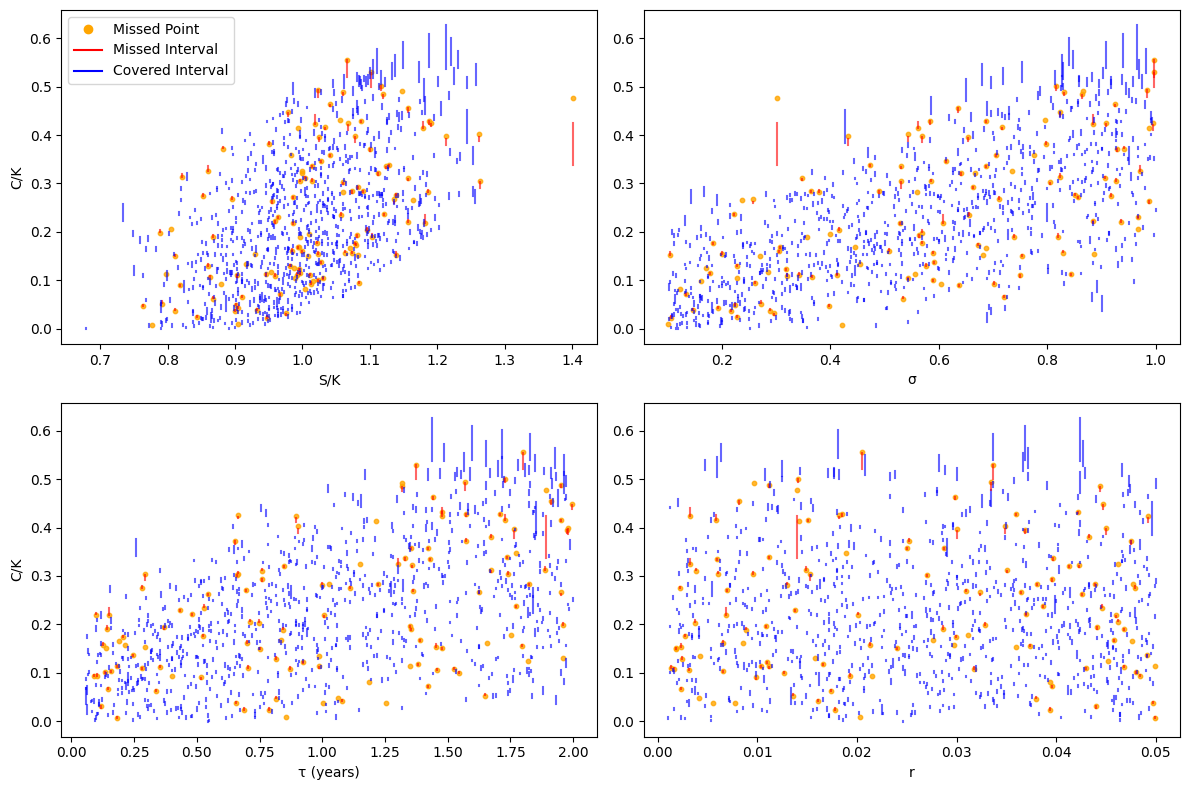
\includegraphics[width=0.8\textwidth]{reports/figures/3.3-nm-figures/sample_5/CQR_PIs_5.png}
    \caption{CQR prediction intervals for 200,000 samples. Covered intervals are shown in blue, missed intervals in red, and missed points in orange. Every 500th data point plotted.}
    \label{fig:CQR_PIs_5}
\end{figure}

%\todo Perhaps comment on how considering this plot for a particular stock across moneyness values and multiplying the predicted C/K by K should reproduce the option pricing curve over time for that underlying. [Miroslav: skip, no time]

\subsubsection{Conditional Coverage}
% this must be stated CONDITIONAL ON something like a range of values of feature(s). You are computing missed rate per bin, not for the entire dataset at once (ie. unconditionally), and this is the key thing! It is hard, if not impossible to have conditional coverage.
% add one sentence about limits of conditional coverage, as in bastos, but there is more in chapter 4 from \cite{angelopoulos2024theoretical-foundations-cp}
Conditional coverage is a metric that evaluates the reliability of prediction intervals by focusing on specific regions of the feature space. By conducting localized analyses, it provides a more detailed understanding of how prediction intervals perform under varying conditions defined by values of specific input features.

\begin{definition}
\textbf{Conditional coverage} quantifies the reliability of prediction intervals within particular subsets of the feature space:
\begin{equation}
\Pr\left(Y_{n+1} \in C(X_{n+1}) \mid X_{n+1} = x \right) \geq 1 - \alpha.
\end{equation}
Here, $C(X_{n+1})$ represents the prediction interval, and $Y_{n+1}$ denotes the true response. This formulation, known as \textbf{pointwise conditional coverage}, ensures that for a specific feature value $x$, the prediction interval captures the true response with a probability of at least $1 - \alpha$. However, evaluating this exact property across the entire continuous feature space is computationally infeasible. Instead, it is common to evaluate conditional coverage over a range or subset of feature values:
\begin{equation}
\Pr\left(Y_{n+1} \in C(X_{n+1}) \mid X_{n+1} \in N \right) \geq 1 - \alpha,
\end{equation}
where $N$ denotes a range or bin of feature values. This is referred to as \textbf{binned conditional coverage}, which provides a practical means of evaluating coverage by aggregating feature values into discretized bins.
\end{definition}

The distinction between these two forms of conditional coverage lies in their granularity. Pointwise conditional coverage ensures the reliability of individual feature values, making it theoretically ideal but impractical in terms of computational resources. On the other hand, binned conditional coverage focuses on a subset of the feature space, providing a more approximate yet practical measure of reliability. According to Chapter 4 of \cite{angelopoulos2024theoretical-foundations-cp}, achieving exact pointwise conditional coverage in a continuous feature space is generally infeasible due to the infinite granularity of such spaces. As such, binned coverage offers a more reasonable alternative.

To approximate conditional coverage, the feature space is divided into bins, and coverage statistics are computed for each bin. This approach is called \textbf{binned conditional coverage}, and it is useful for identifying regions where prediction intervals underperform, helping to pinpoint areas where the model needs to be improved or additional data should be collected.

\begin{definition}
A complementary metric to binned conditional coverage is the \textbf{missed rate}, which quantifies the proportion of prediction intervals within each bin that fail to capture the true response:
\begin{equation}
\text{Missed Rate}_B = \frac{\text{Missed Intervals in } B}{\text{Total Intervals in } B},
\end{equation}
where $B$ is a range of feature values such that $X_{n+1} \in B$. The missed rate and conditional coverage are directly related by the equation:
\begin{equation}
\text{Missed Rate}_B = 1 - \text{Conditional Coverage}_B.
\end{equation}
\end{definition}

By examining missed rates across feature bins, one can gain insights into the local reliability of prediction intervals while avoiding the challenges of strict pointwise conditional coverage. The missed rate provides a straightforward measure of failure, highlighting specific regions in the feature space where prediction intervals are less reliable.

The missed rates for CQR with a training sample size of $n_{\text{train}} = 200,000$ are shown in Figure~\ref{fig:CQR_MISSED_RATE_5}. These are calculated across 10 bins for each feature, and the missed rates within each bin are plotted as bar graphs. Results for other training sample sizes and for NQR are included in the appendix.

\begin{figure}[h]
    \centering
    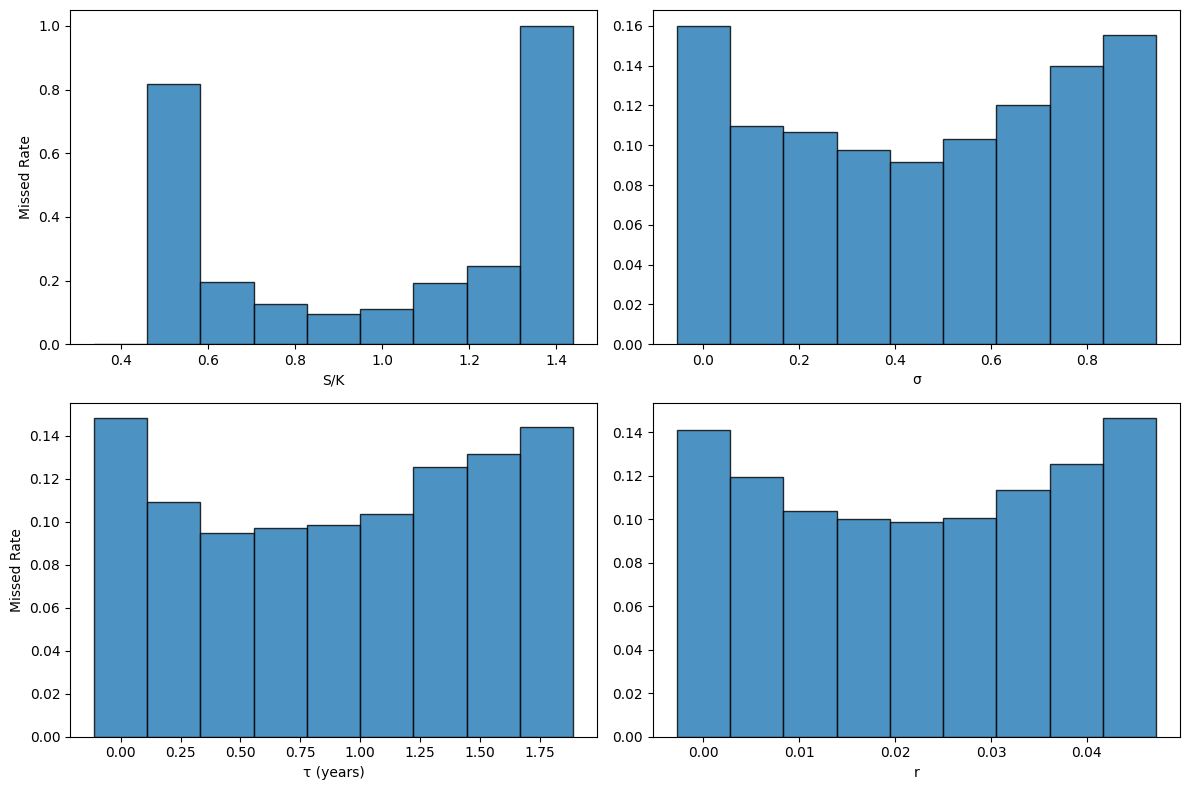
\includegraphics[width=0.8\textwidth]{reports/figures/3.3-nm-figures/sample_5/CQR_MISSED_RATE_5.png}
    \caption{CQR missed rates for 200,000 samples, plotted across 10 bins of moneyness, volatility, time-to-maturity (years), and interest rate.}
    \label{fig:CQR_MISSED_RATE_5}
\end{figure}

The results reveal notable patterns:
\begin{itemize}
    \item \textbf{Moneyness ($S/K$):} Missed rates are highest in the extreme bins, those where $S/K < 0.5$ or $S/K > 1.3$, corresponding to deep in-the-money or far out-of-the-money options. These regions are characterized by sparse data and, presumably, a greater pricing uncertainty. Bins around at-the-money options exhibit significantly reduced missed rates, reflecting better data density and model fit.
    \item \textbf{Volatility ($\sigma$):} A U-shaped pattern emerges, with higher missed rates at both low and high extremes of volatility. This trend reflects the challenges of modeling extreme market conditions, where data is sparse and pricing variability is higher.
    \item \textbf{Time-to-maturity ($\tau$):} Missed rates are higher for the shortest and longest durations, indicating increased uncertainty at these extremes. Slightly elevated missed rates at both ends emphasize the challenges of modeling short-term and long-term maturities.
    \item \textbf{Interest rate ($r$):} Missed rates are higher at extreme values, again likely due to sparse data. A slight dip in the middle bins suggests improved model reliability under moderate interest rates.
\end{itemize}

These results are consistent with theoretical expectations. Sparse regions of the feature space, such as extreme moneyness or volatility, lead to higher missed rates due to insufficient data and increased uncertainty. While binned conditional coverage offers a practical framework for analyzing prediction interval reliability, it remains an approximation of true pointwise conditional coverage.

\subsubsection{Widths of PIs across feature and response space}
% comment based on the basic intuition on why is uncertainty bigger at some points, etc. ANSWER: less training data in this region leading to greater variability in model output, or due to inherent pricing uncertainty (liquidity issues)

Figure \ref{fig:kappa4_rel_widths} shows the distribution of relative widths of prediction intervals across the simulated dataset. While the majority of interval widths are concentrated within the range of $0$ to $20\%$, there are also some intervals with exceptionally wide widths. These outliers in the tail of the distribution reveal regions where the model's predictions are subject to high uncertainty.

The inset in the figure provides a magnified view of the narrower intervals, offering a closer look at their distribution. Narrow intervals correspond to areas where the model benefits from sufficient training data or where the relationship between features and responses is relatively stable. Conversely, wider intervals are related to situations where training data is scarce or uncertainty is inherently high, such as in illiquid markets or options with extreme characteristics.

\begin{figure}[H]
\centering
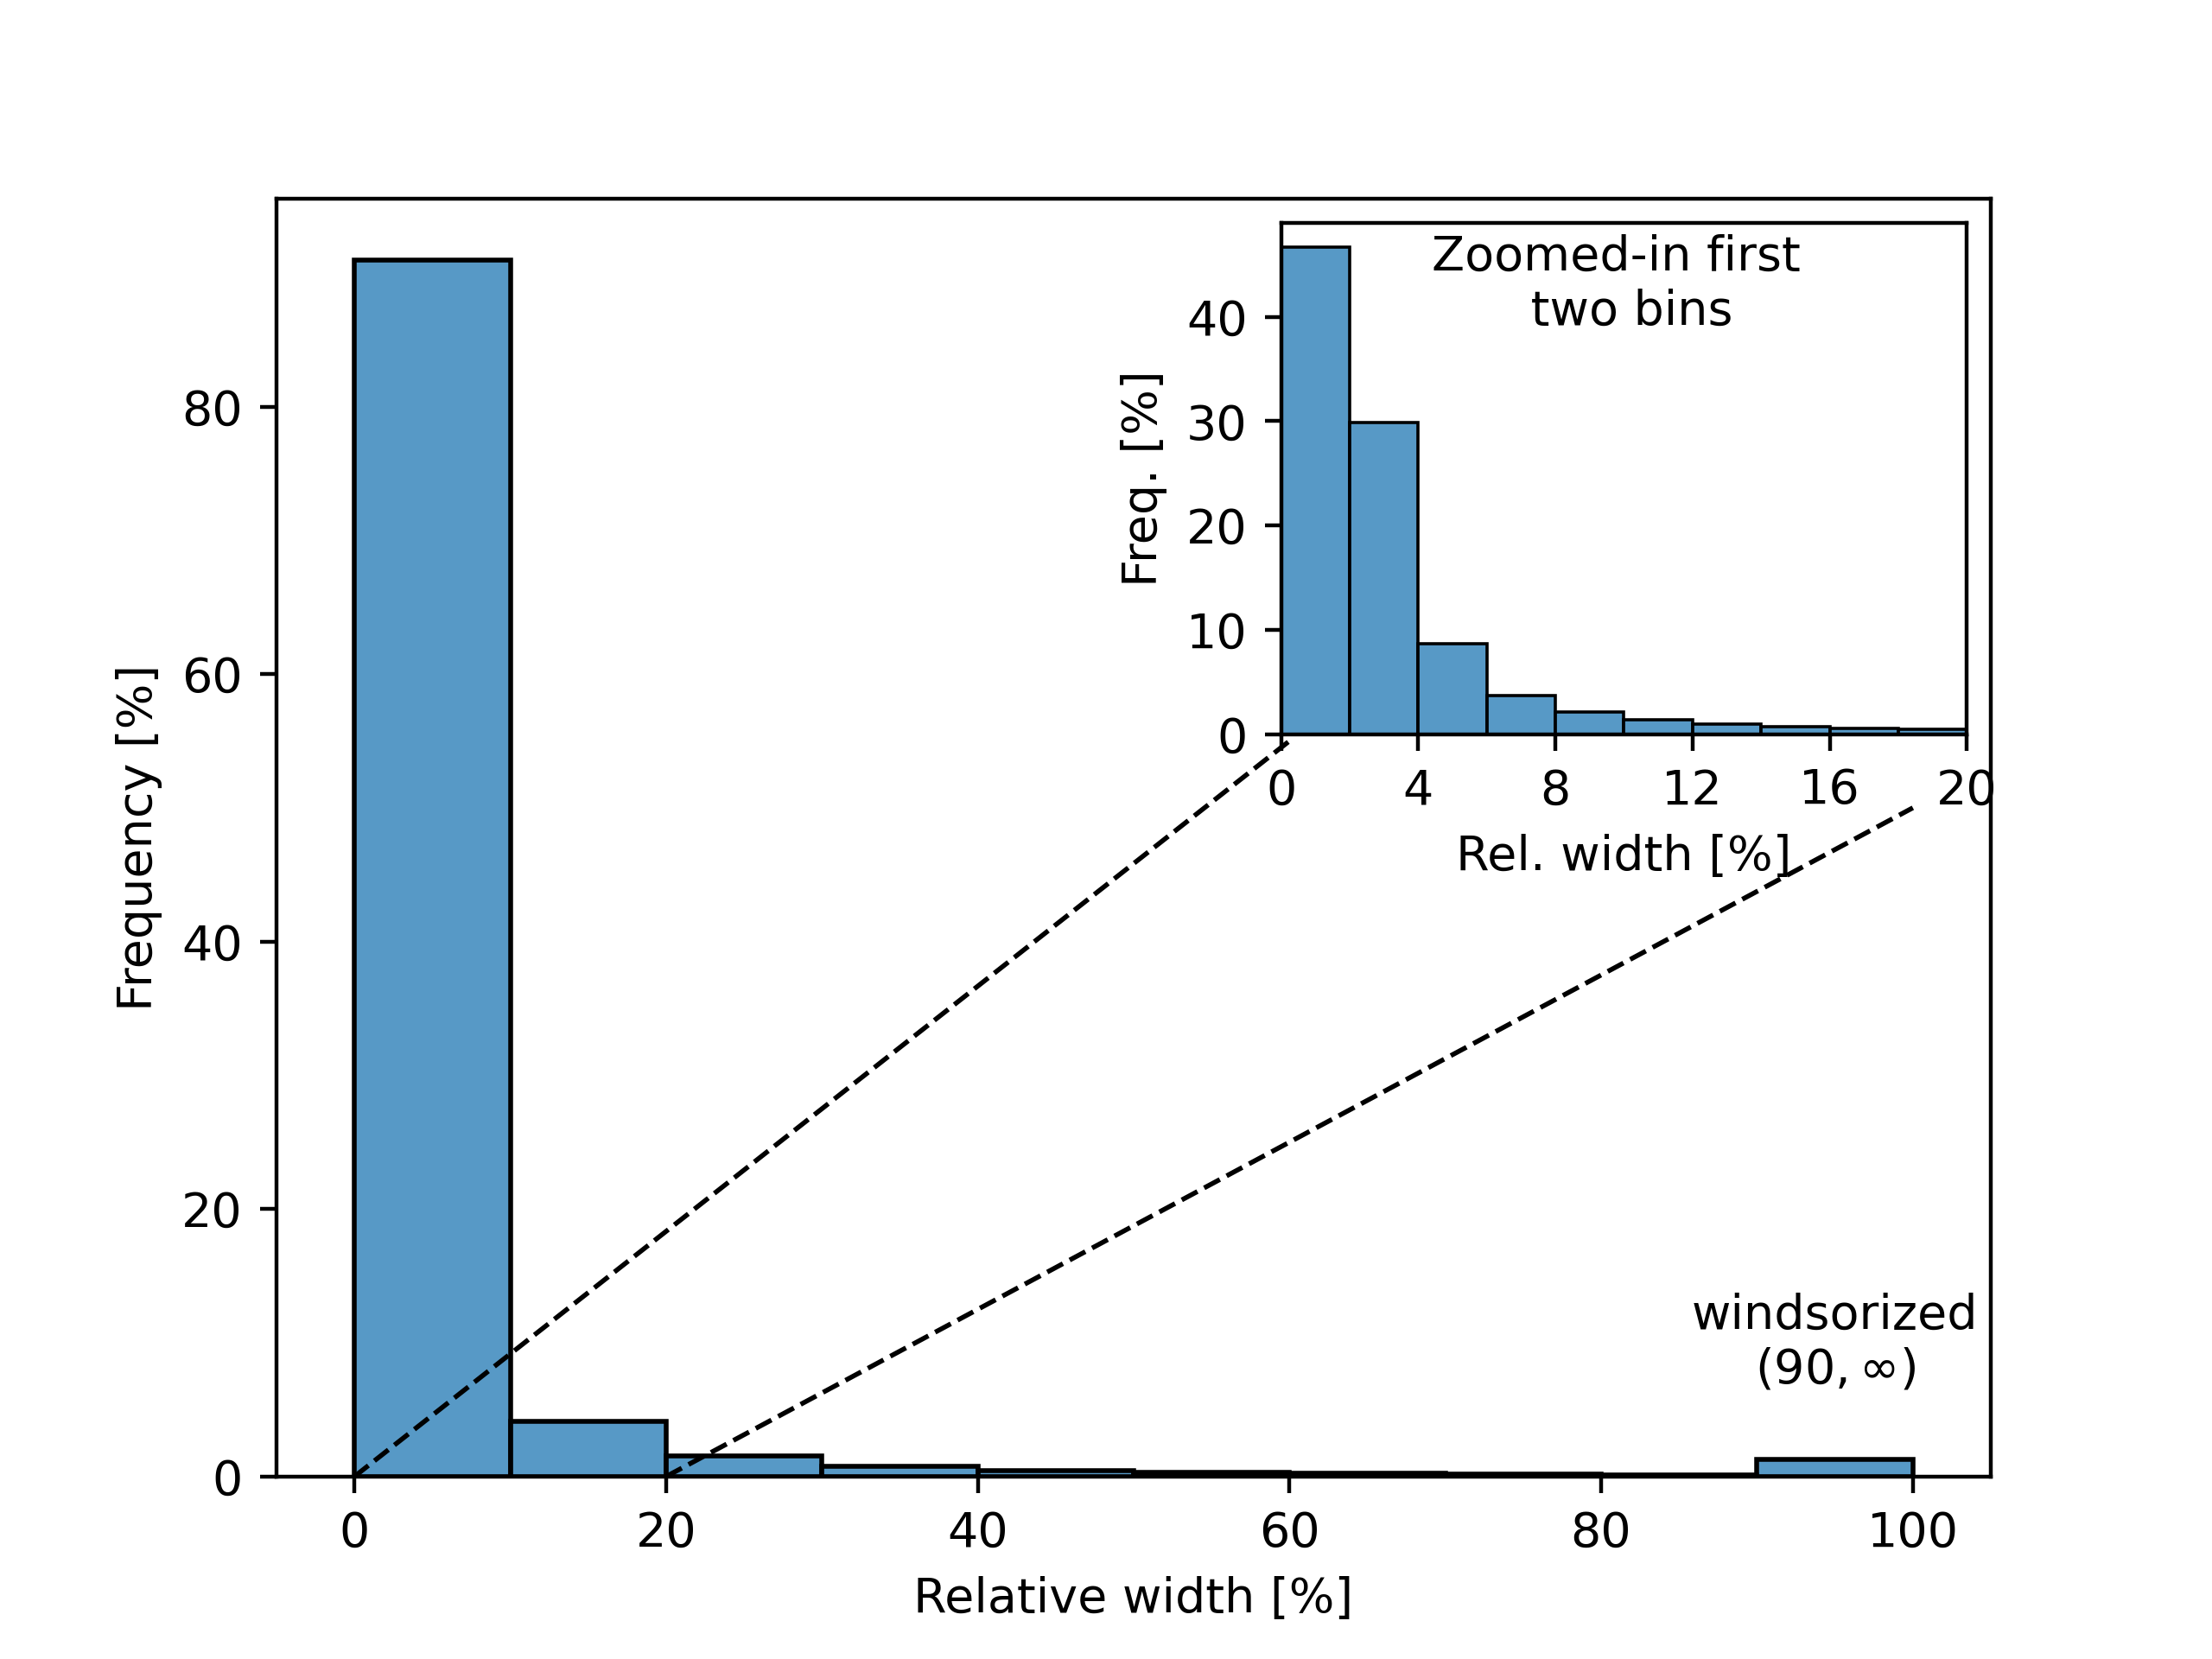
\includegraphics[width=0.8\textwidth]{reports/figures/simulated_data/sim_kappa4_relative_widths.png}
\caption{Distributions of relative widths of PIs for $\kappa=4$.}
\label{fig:kappa4_rel_widths}
\end{figure}

The median relative interval width quantifies the central tendency of prediction interval widths relative to the true label. For each data point, the relative width is given by $ (U - L) / \text{True Label} $, where $U$ and $L$ are the upper and lower bounds of the prediction interval. The measure is the median of these relative widths, providing a summary of predictive uncertainty.

Figure \ref{fig:kappa4_rel_widths_vs_features} examines how the widths of prediction intervals change depending on different features:

\begin{itemize}
    \item \textbf{Moneyness ($S/K$):} There is a clear pattern in the widths of the intervals, with options that have extreme moneyness, i.e., those that are deeply in-the-money or far out-of-the-money, exhibiting wider intervals. This can be attributed to the fact that such options are traded infrequently, resulting in a lack of sufficient training data. Moreover, their heightened sensitivity to market dynamics amplifies the uncertainty in pricing. In contrast, at-the-money options have narrower interval widths, reflecting higher confidence in the model’s predictions.
    \item \textbf{Volatility ($\sigma$):} Higher levels of volatility lead to wider intervals, as pronounced price fluctuations increase unpredictability. This is a common challenge in pricing models, where higher volatility exacerbates forecast uncertainty.
    \item \textbf{Time-to-maturity ($\tau$):} Options approaching expiration tend to have wider intervals, often due to the rapid price movements observed in the final days before expiry, a phenomenon linked to pin risk~\cite{GOLEZ2012566}. Whereas options with shorter time-to-maturity experience greater uncertainty, the prediction intervals for long-term options are narrower, as more stable, long-term market factors influence their prices.
    \item \textbf{Interest rate ($r$):} The widths of intervals across different interest rates remain relatively stable, indicating that the impact of interest rates on pricing uncertainty is minimal for short-term options.
\end{itemize}

\begin{figure}[H]
\centering
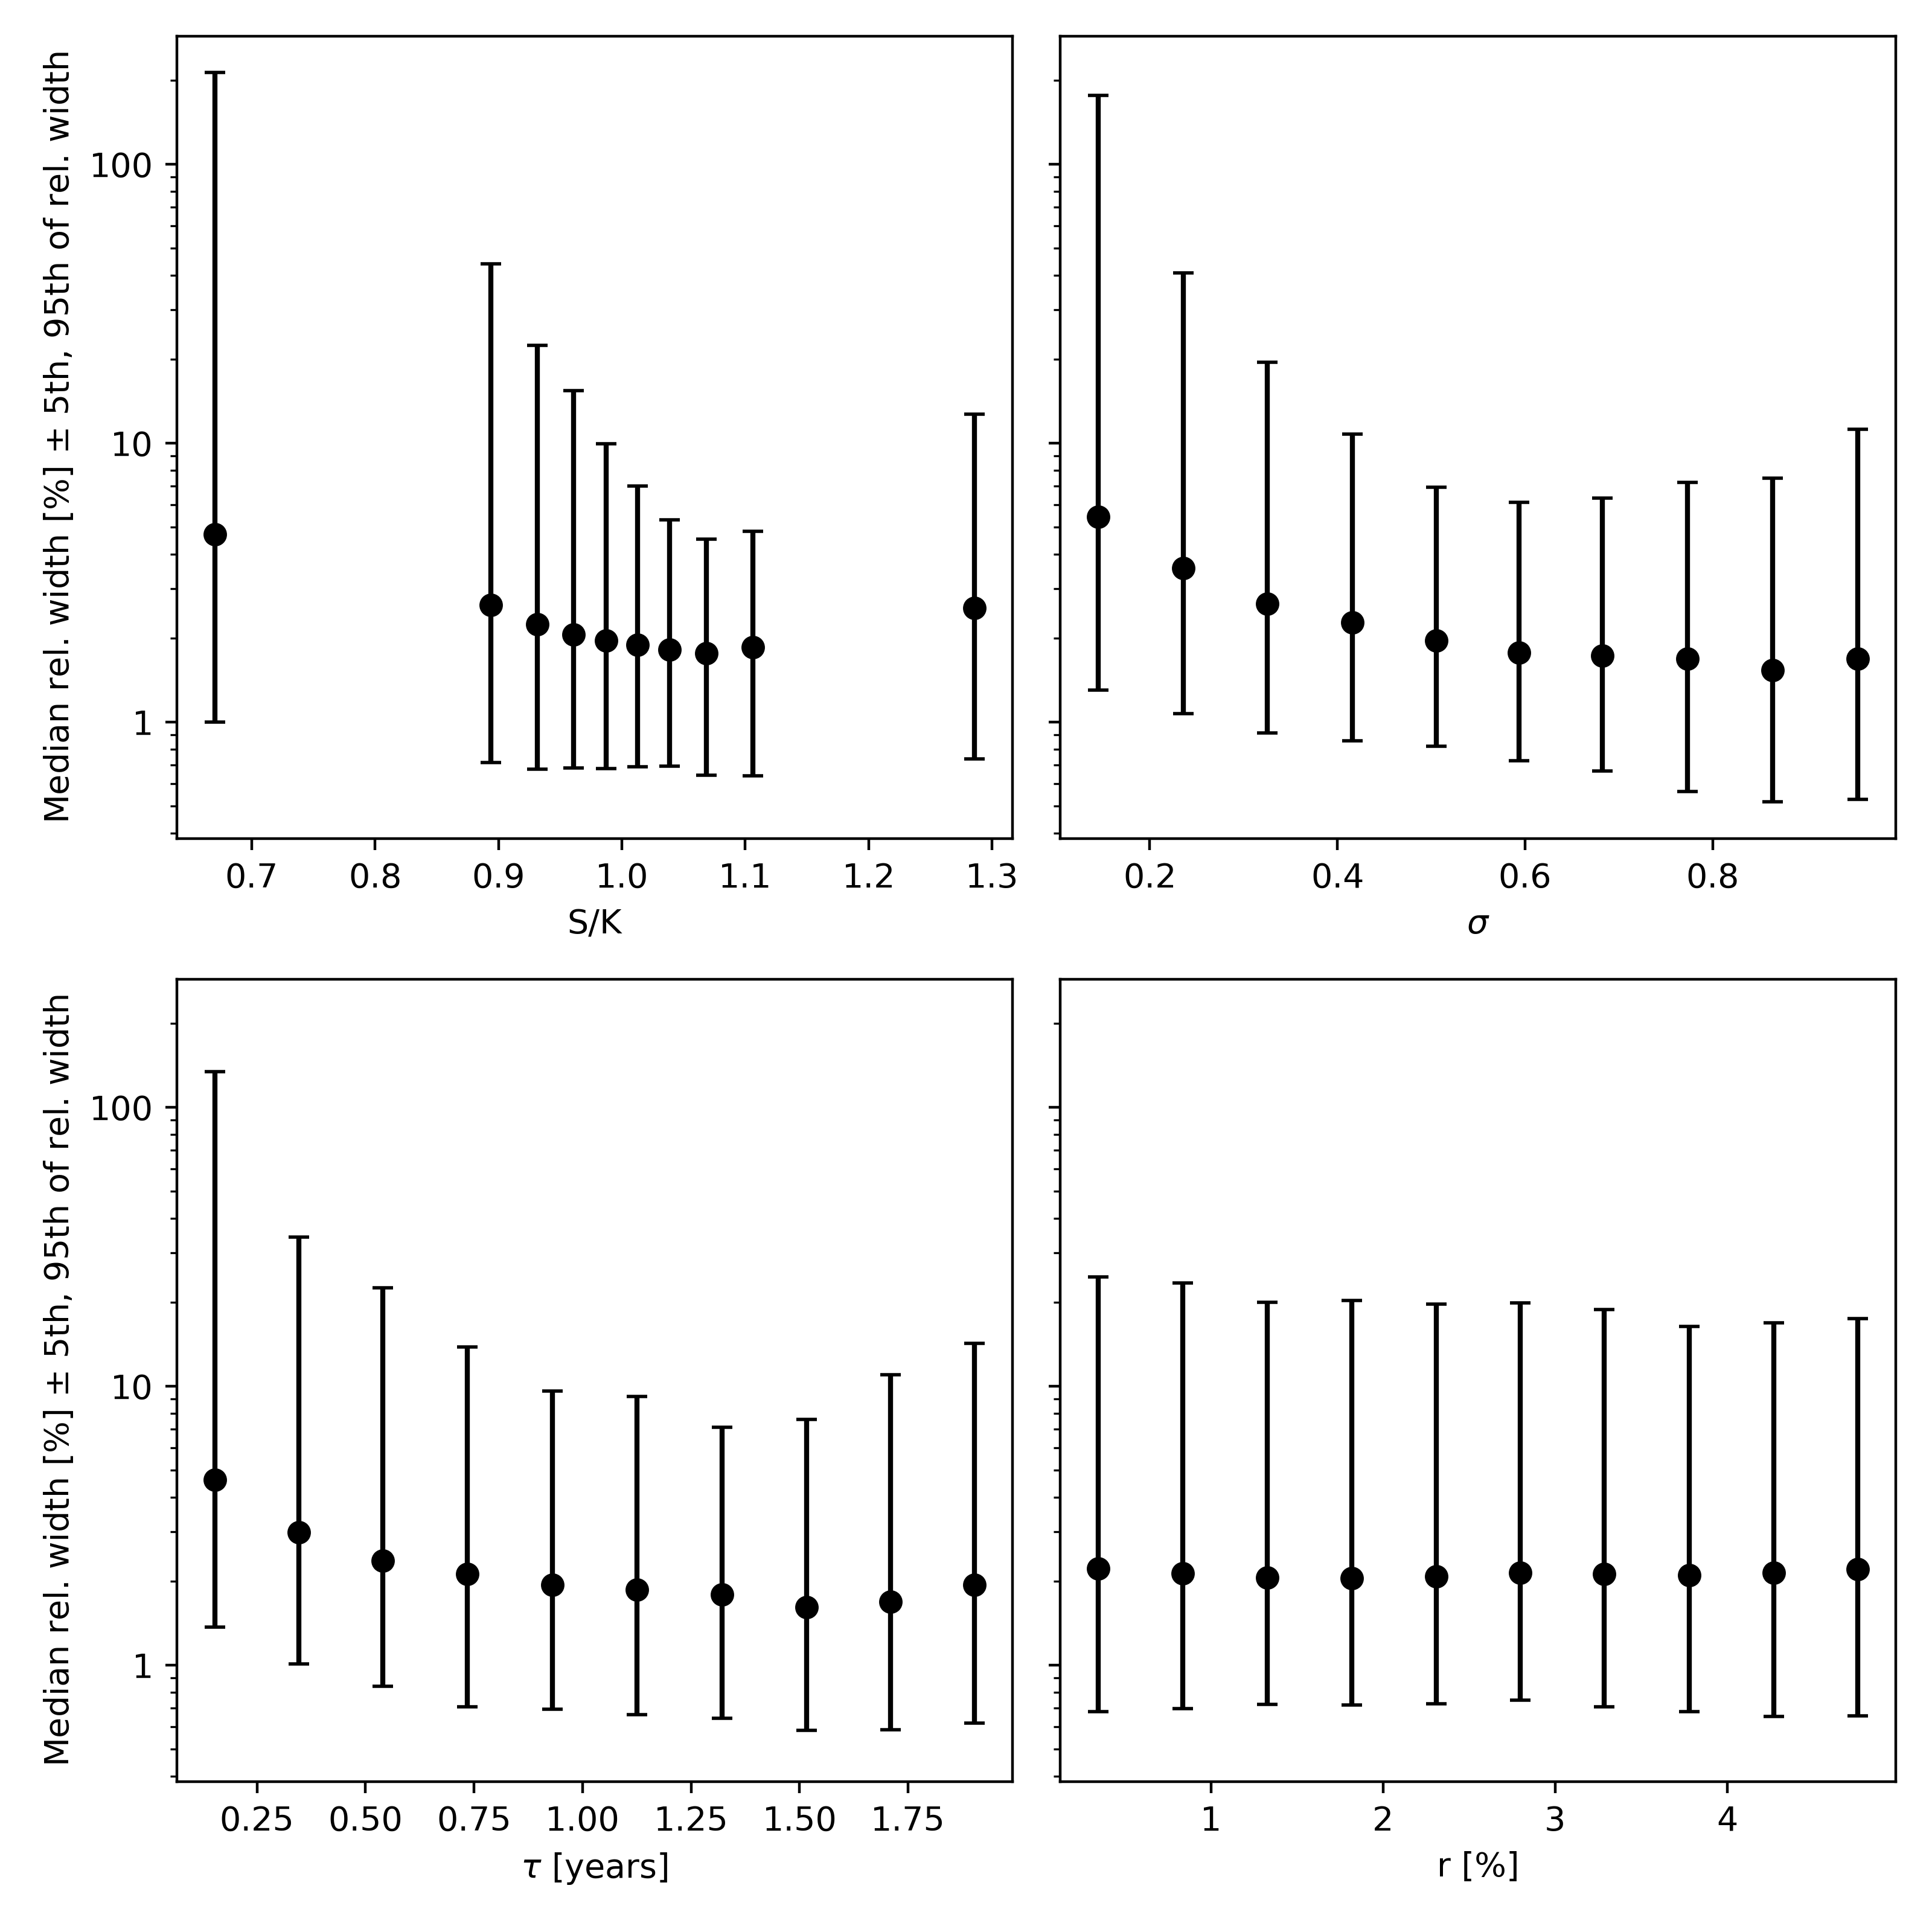
\includegraphics[width=0.8\textwidth]{reports/figures/simulated_data/sim_kappa4_rel_widths_to_features.png}
\caption{Relative widths of PIs accross features for $\kappa=4$.}
\label{fig:kappa4_rel_widths_vs_features}
\end{figure}

Figure \ref{fig:kappa4_rel_widths_vs_option_price} analyzes the relationship between normalized option prices and prediction interval widths. For options with very low normalized prices, the relative widths of the intervals appear significantly larger. This behavior arises primarily because dividing by small true label values results in disproportionately large relative widths, combined with the inherent difficulty in accurately pricing deep out-of-the-money options.

As normalized prices increase toward more typical values, the interval widths stabilize and become narrower. This trend reflects the availability of more robust training data and the reduced volatility associated with mid-range option prices. The error bars highlight the variability in interval widths across different price levels, with extreme price ranges exhibiting both larger median widths and greater variability.

\begin{figure}[H]
\centering
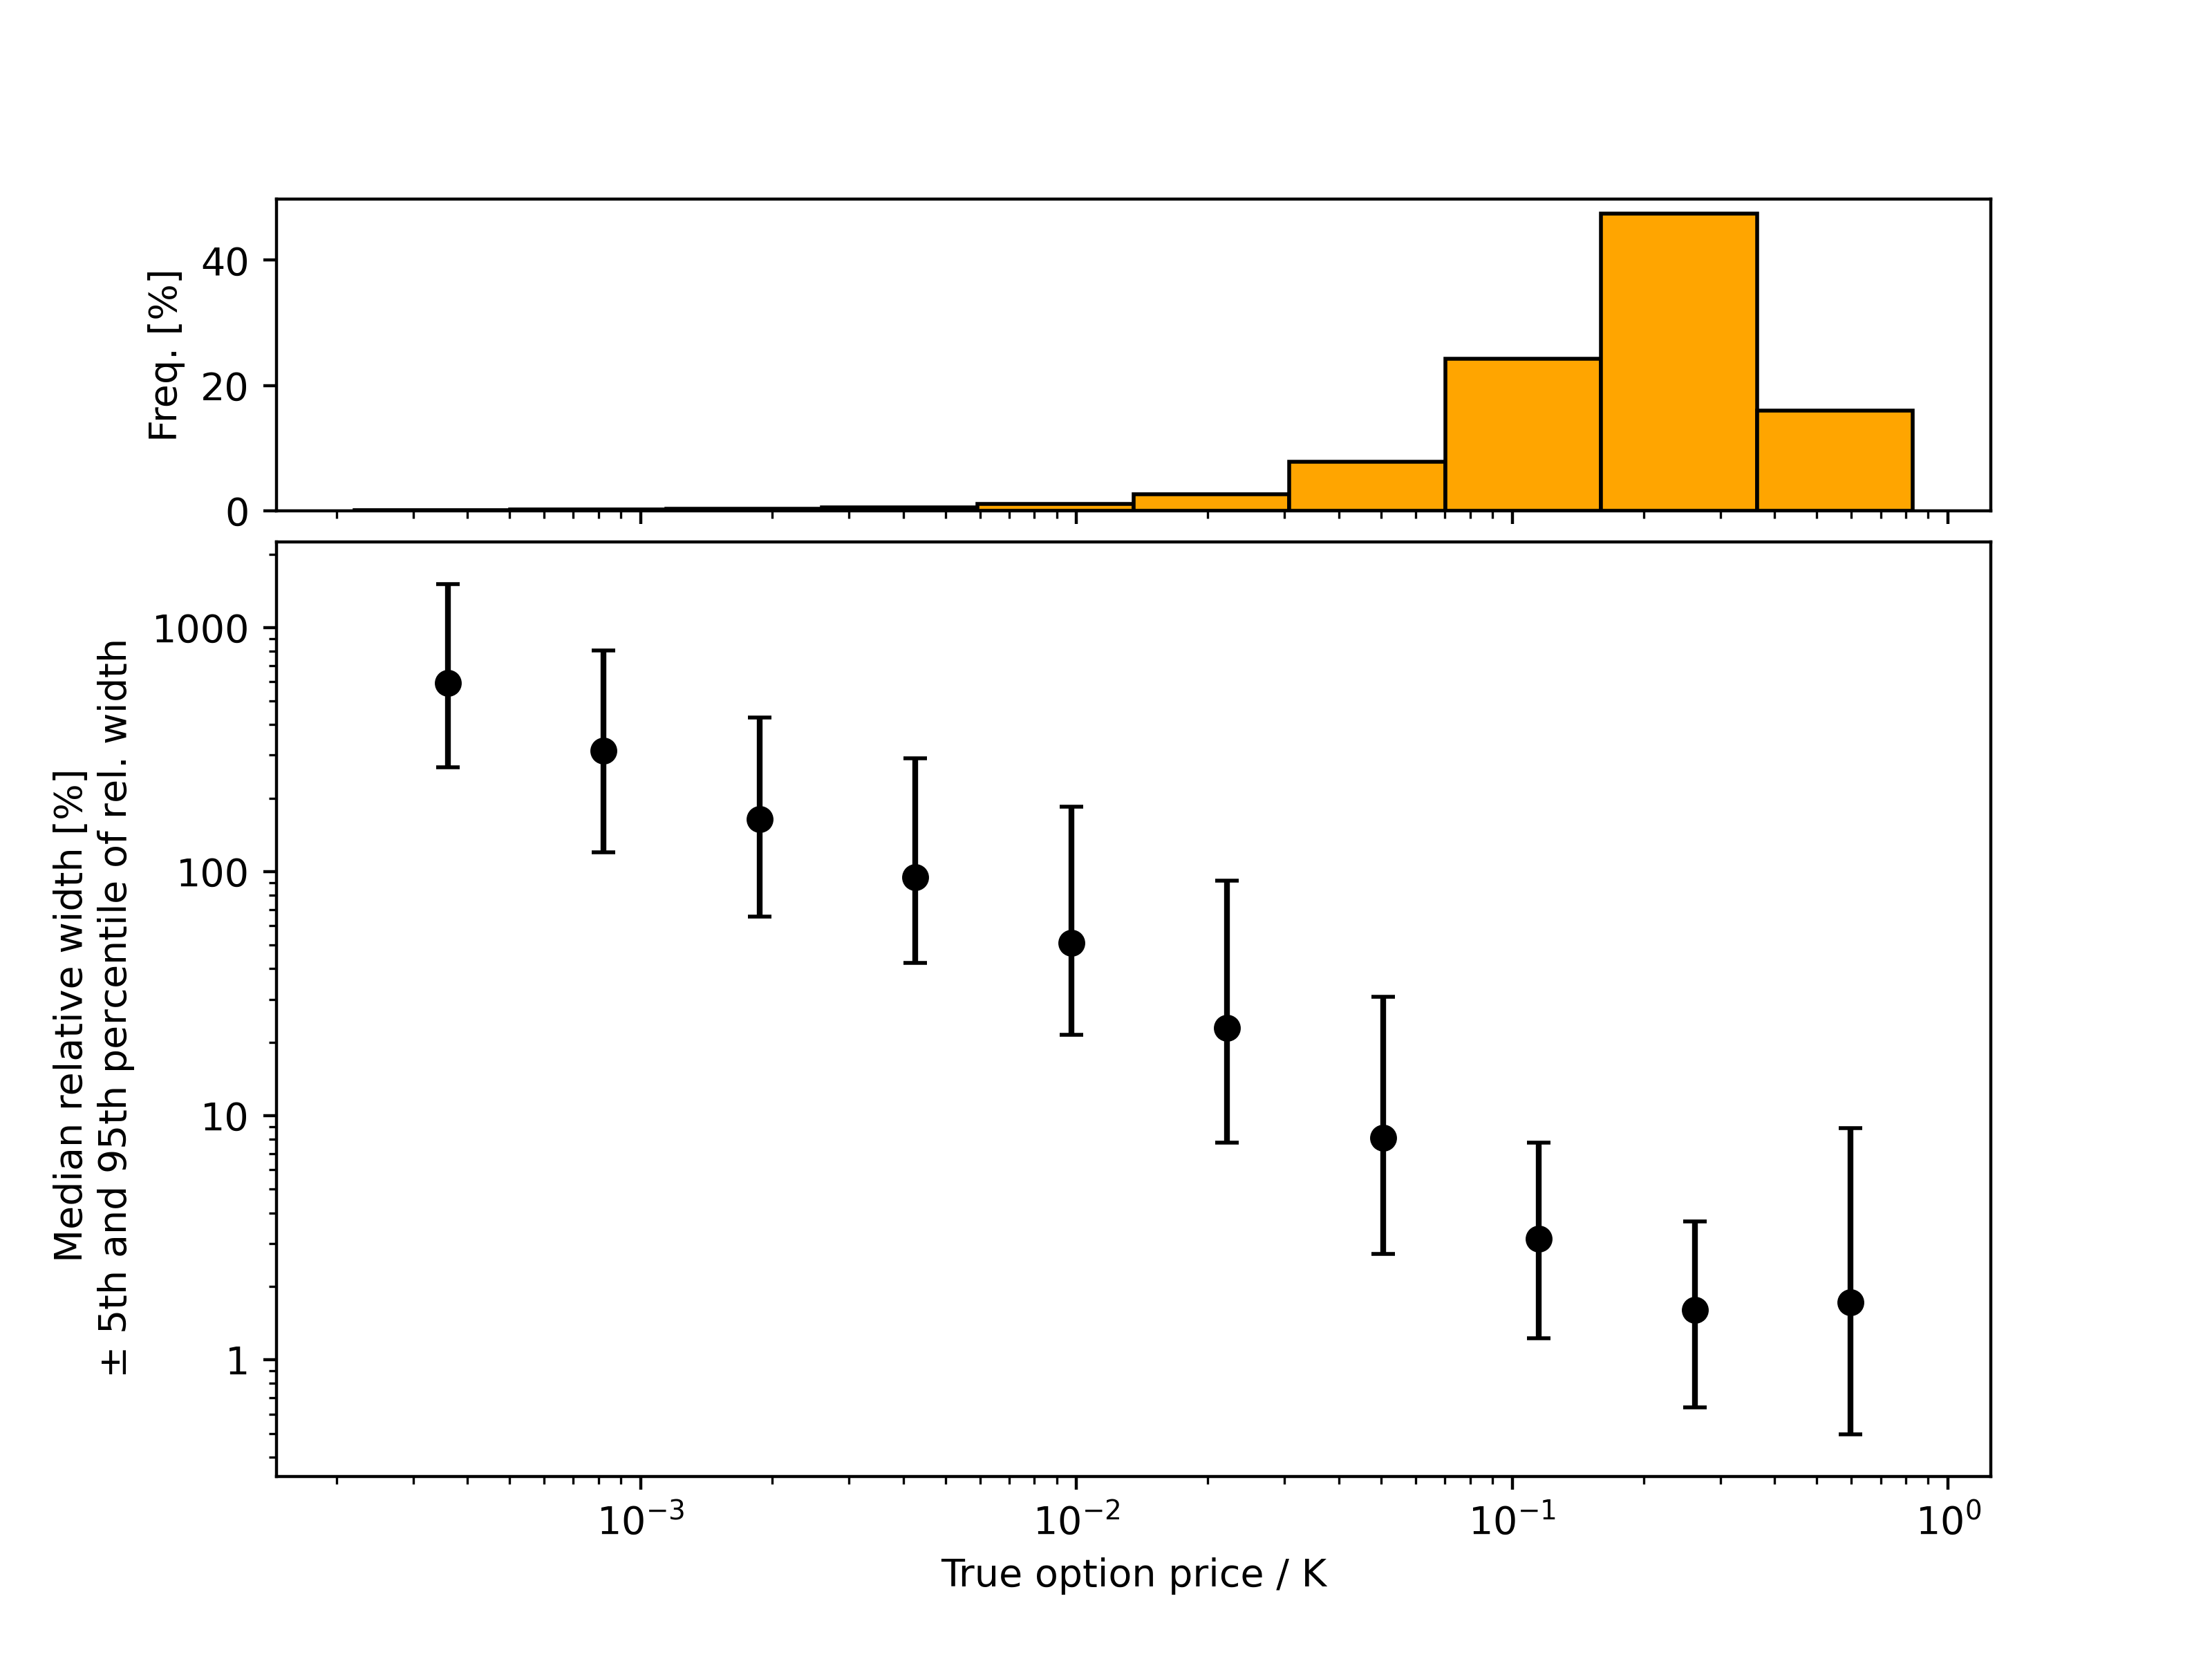
\includegraphics[width=0.8\textwidth]{reports/figures/simulated_data/sim_kappa4_rel_widths_to_opt_price.png}
\caption{PIs binned by the value of the target variable for $\kappa=4$.}
\label{fig:kappa4_rel_widths_vs_option_price}
\end{figure}

The notebooks \texttt{3.0-mz-confirmalize.ipynb} and \texttt{3.2-nm-figures-mapie.ipynb} document the construction of CQR on simulated data using MAPIE package~\cite{Cordier_Flexible_and_Systematic_2023}. In the notebooks \texttt{3.1-mz-sim-data-analy\allowbreak sis.ipynb}; \texttt{3.2-nm-figures-mapie.ipynb} and 
\texttt{3.3-nm-figures.ipynb} we analyzed predictions of the PIs on the test data. 



\section{Replication of Results with Real Data} \label{sec:real1}

\subsection{Data preprocessing}
To accurately learn the pricing function data must be cleaned to reflect a consistent pricing mechanism. The same procedure is followed as in \cite{bastos} using the WRDS OptionMetrics database. Data is initially collected for daily stock prices of the 8 stocks Amazon, AMD, Boeing, Disney, Meta, Netflix, Paypal, and Salesforce from the S\&P 500 between November 11th, 2020, and February 12th, 2021. The important data here is the date, security id, and daily close price, which is used to represent the spot price. In addition to this, the relevant daily zero-curve and option data are also required. The zero curve includes the interest rate across several tenors at a particular date. For the options data we only consider American Call options and require the security id, date, strike price, expiry date, best bid, best offer, and implied volatility. The price of an option is taken to be the average of the best bid and offer, and the time to maturity is of course the difference between the expiry date and current date. Thus, matching data across date and security id allows us to obtain values for $(S, K, \sigma, \tau, V)$. The appropriate risk-free interest rate $r$ is then found by the following procedure: For a specific date, compare the $\tau$ of the option to the tenors of the zero curve. If there is an interest rate tenor matching this time to expiry, that rate is used for $r$. In the case that there is no tenor directly matching $\tau$ and the time to expiry of the option instead falls between two interest rate tenors, $t_1 < \tau < t_2$, then $r$ is taken to be the linearly interpolated value of the rates corresponding to these two tenors, i.e. $r = r_1 + (\tau-t_1)*(r_2 - r_1)/(t_2-t_1)$. 

Before calculating and collating the required pricing parameters, the data is naturally cleaned to remove data with missing values. In order for the ML model to learn the appropriate pricing function, further cleaning is done to neglect data corresponding to inaccurate pricing. Liquidity is therefore a valuable filter, as illiquid options are more likely to be poorly priced. For example, deep ITM or OTM tend to have extremely poor liquidity with large spreads. A further consideration is that options close to maturity are rarely traded. Therefore, options with moneyness $S/K > 1.5$ and $S/K < 0.5$ as well as time to expiry $\tau < \text{10 days}$ are removed. Data without posted bids represented as zeros are additionally neglected. Hence, the required training data $\mathcal{D}$ is collated as a table with values $(S, \sigma, \tau, r, K, V)$ corresponding to options assumed to be priced consistently and accurately.

In the figure \ref{fig:real1_features_dist} of the appendix, we present histograms of real data used in this section. Note that due to floating point errors, 0.8\% of deep in the money calls were included, but this should not degrade performance. To fix this, all floating point numbers should be ensured to retain as much accuracy as possible.

Code for fetching and preprocessing real data is presented in notebooks \texttt{4.0-mz-sp500\_constituents.ipynb} for fetching constituents lists for S\&P500. This code is kindly provided by Patrick Lucescu. Notebook \texttt{4.1-mz-fetch-replication-data.ipynb} and \texttt{4.2-mz-fetch-big-dataset.ipynb} document fetching data for this section and the next section. Lastly, data cleaning is documented in the notebook \texttt{4.3-mz-clean-big-dataset.ipynb}. Additional scripts, such as SQLite scripts for data cleaning, are available in \texttt{src\/real\_data\/} directory in the project files.

\subsection{Results}

Figure \ref{fig:real1_coverage_hist} represents empirical coverage computed using 100 different random splits. We can see that empirical coverage is near the nominal level, and variation due to the randomness of the split is negligible. This indicates that the loss of coverage that happens when we do not use a random splitting is, indeed, due to lost exchangeability - not by a chance of choosing a particular random split. 

\begin{figure}
\centering
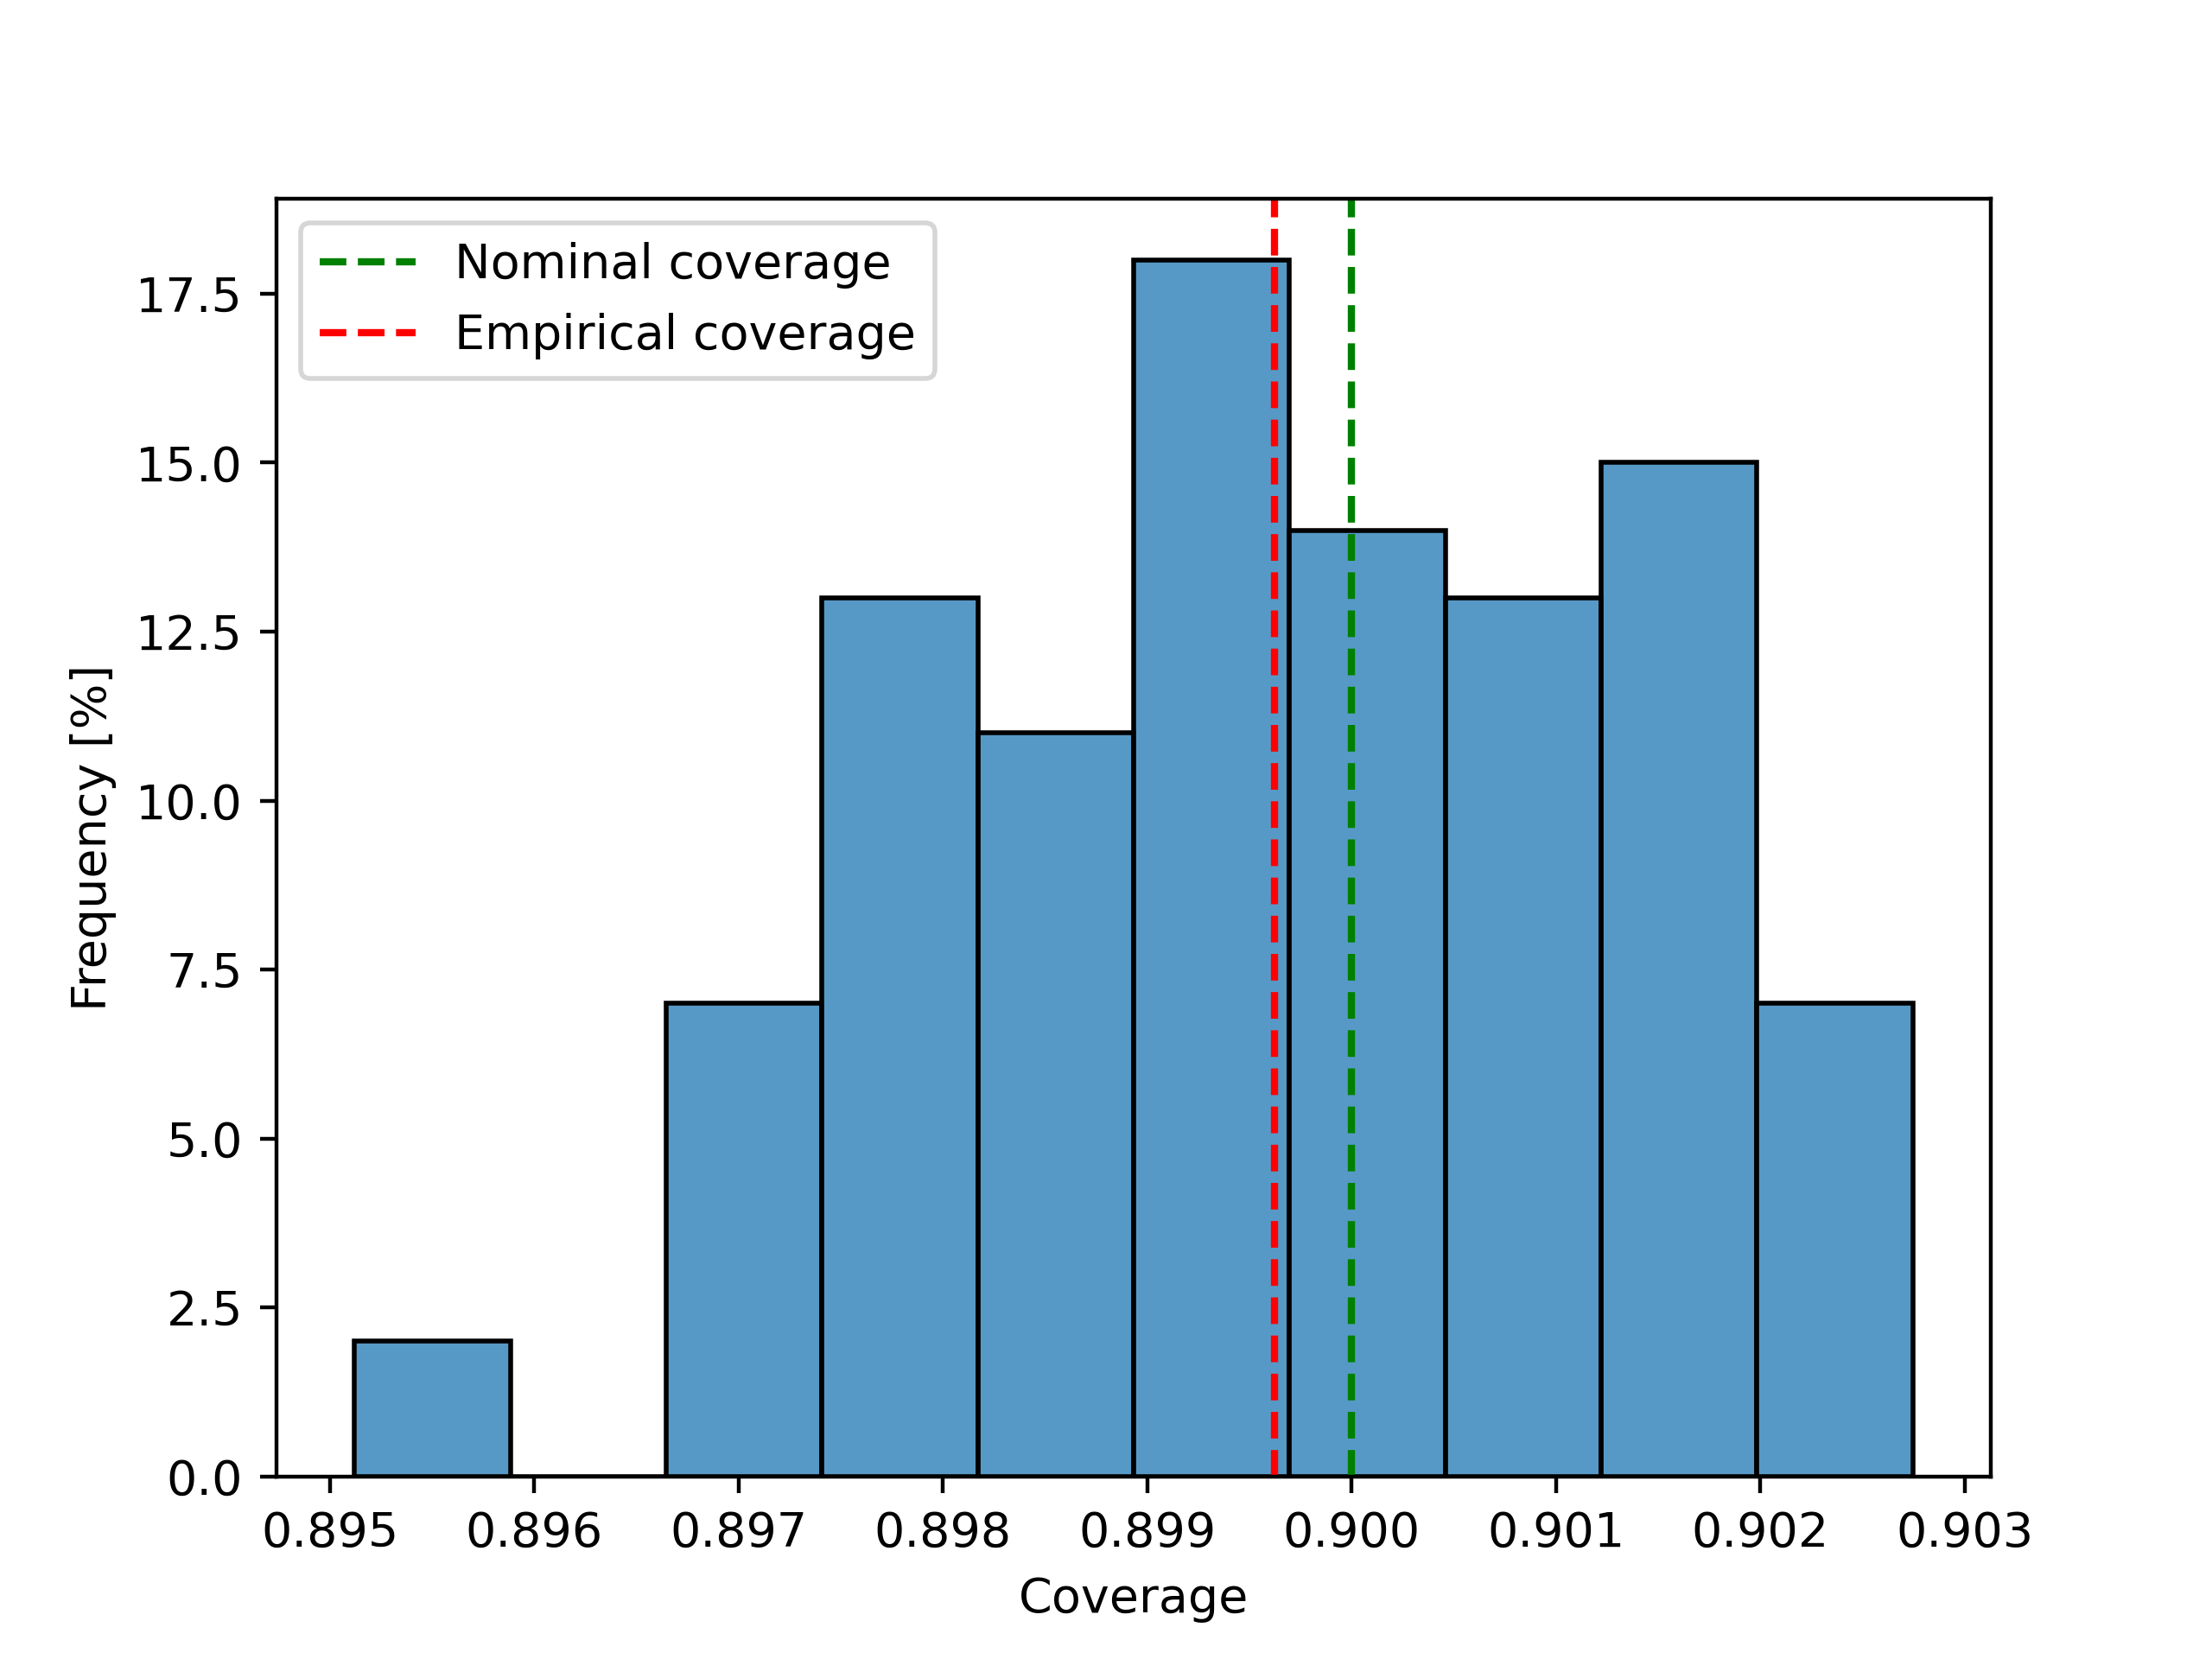
\includegraphics[width=0.6\textwidth]{reports/figures/real_data_replication/real1_coverage_hist.png}
\caption{Empirical coverage on the test set, computed for 100 different random data splits. Dataset: Section \ref{sec:real1}.}
\label{fig:real1_coverage_hist}
\end{figure}

Figure \ref{fig:real1_rel_widths_vs_features} shows median relative widths of PIs, computed on binned data points, where binning is done into 10 different groups (0th to 10th quantile, 10th to 20th quantile, etc.) by the 4 different features. The lower the median relative width is, the lower the uncertainty of predictions in that bin. We see that deep out-of-the-money options have higher price uncertainty; higher implied volatility leads to a higher price uncertainty; shorter maturities have higher price uncertainty - all of which are expected behaviors.

Somewhat surprising is that lower interest rates have higher price uncertainty. During the period of time for which the data was collected (November 11th, 2020, to February 12th, 2021), the FED key policy interest rate has been kept constant at 0.25\%. The variability of interest rates in this dataset is more due to calculations of effective interest rates for different maturities than it is due to fluctuations observed on the market. Thus, behavior with respect to interest rate for this dataset is expected to be aligned with the behavior with respect to time-to-maturity. 

\begin{figure}
\centering
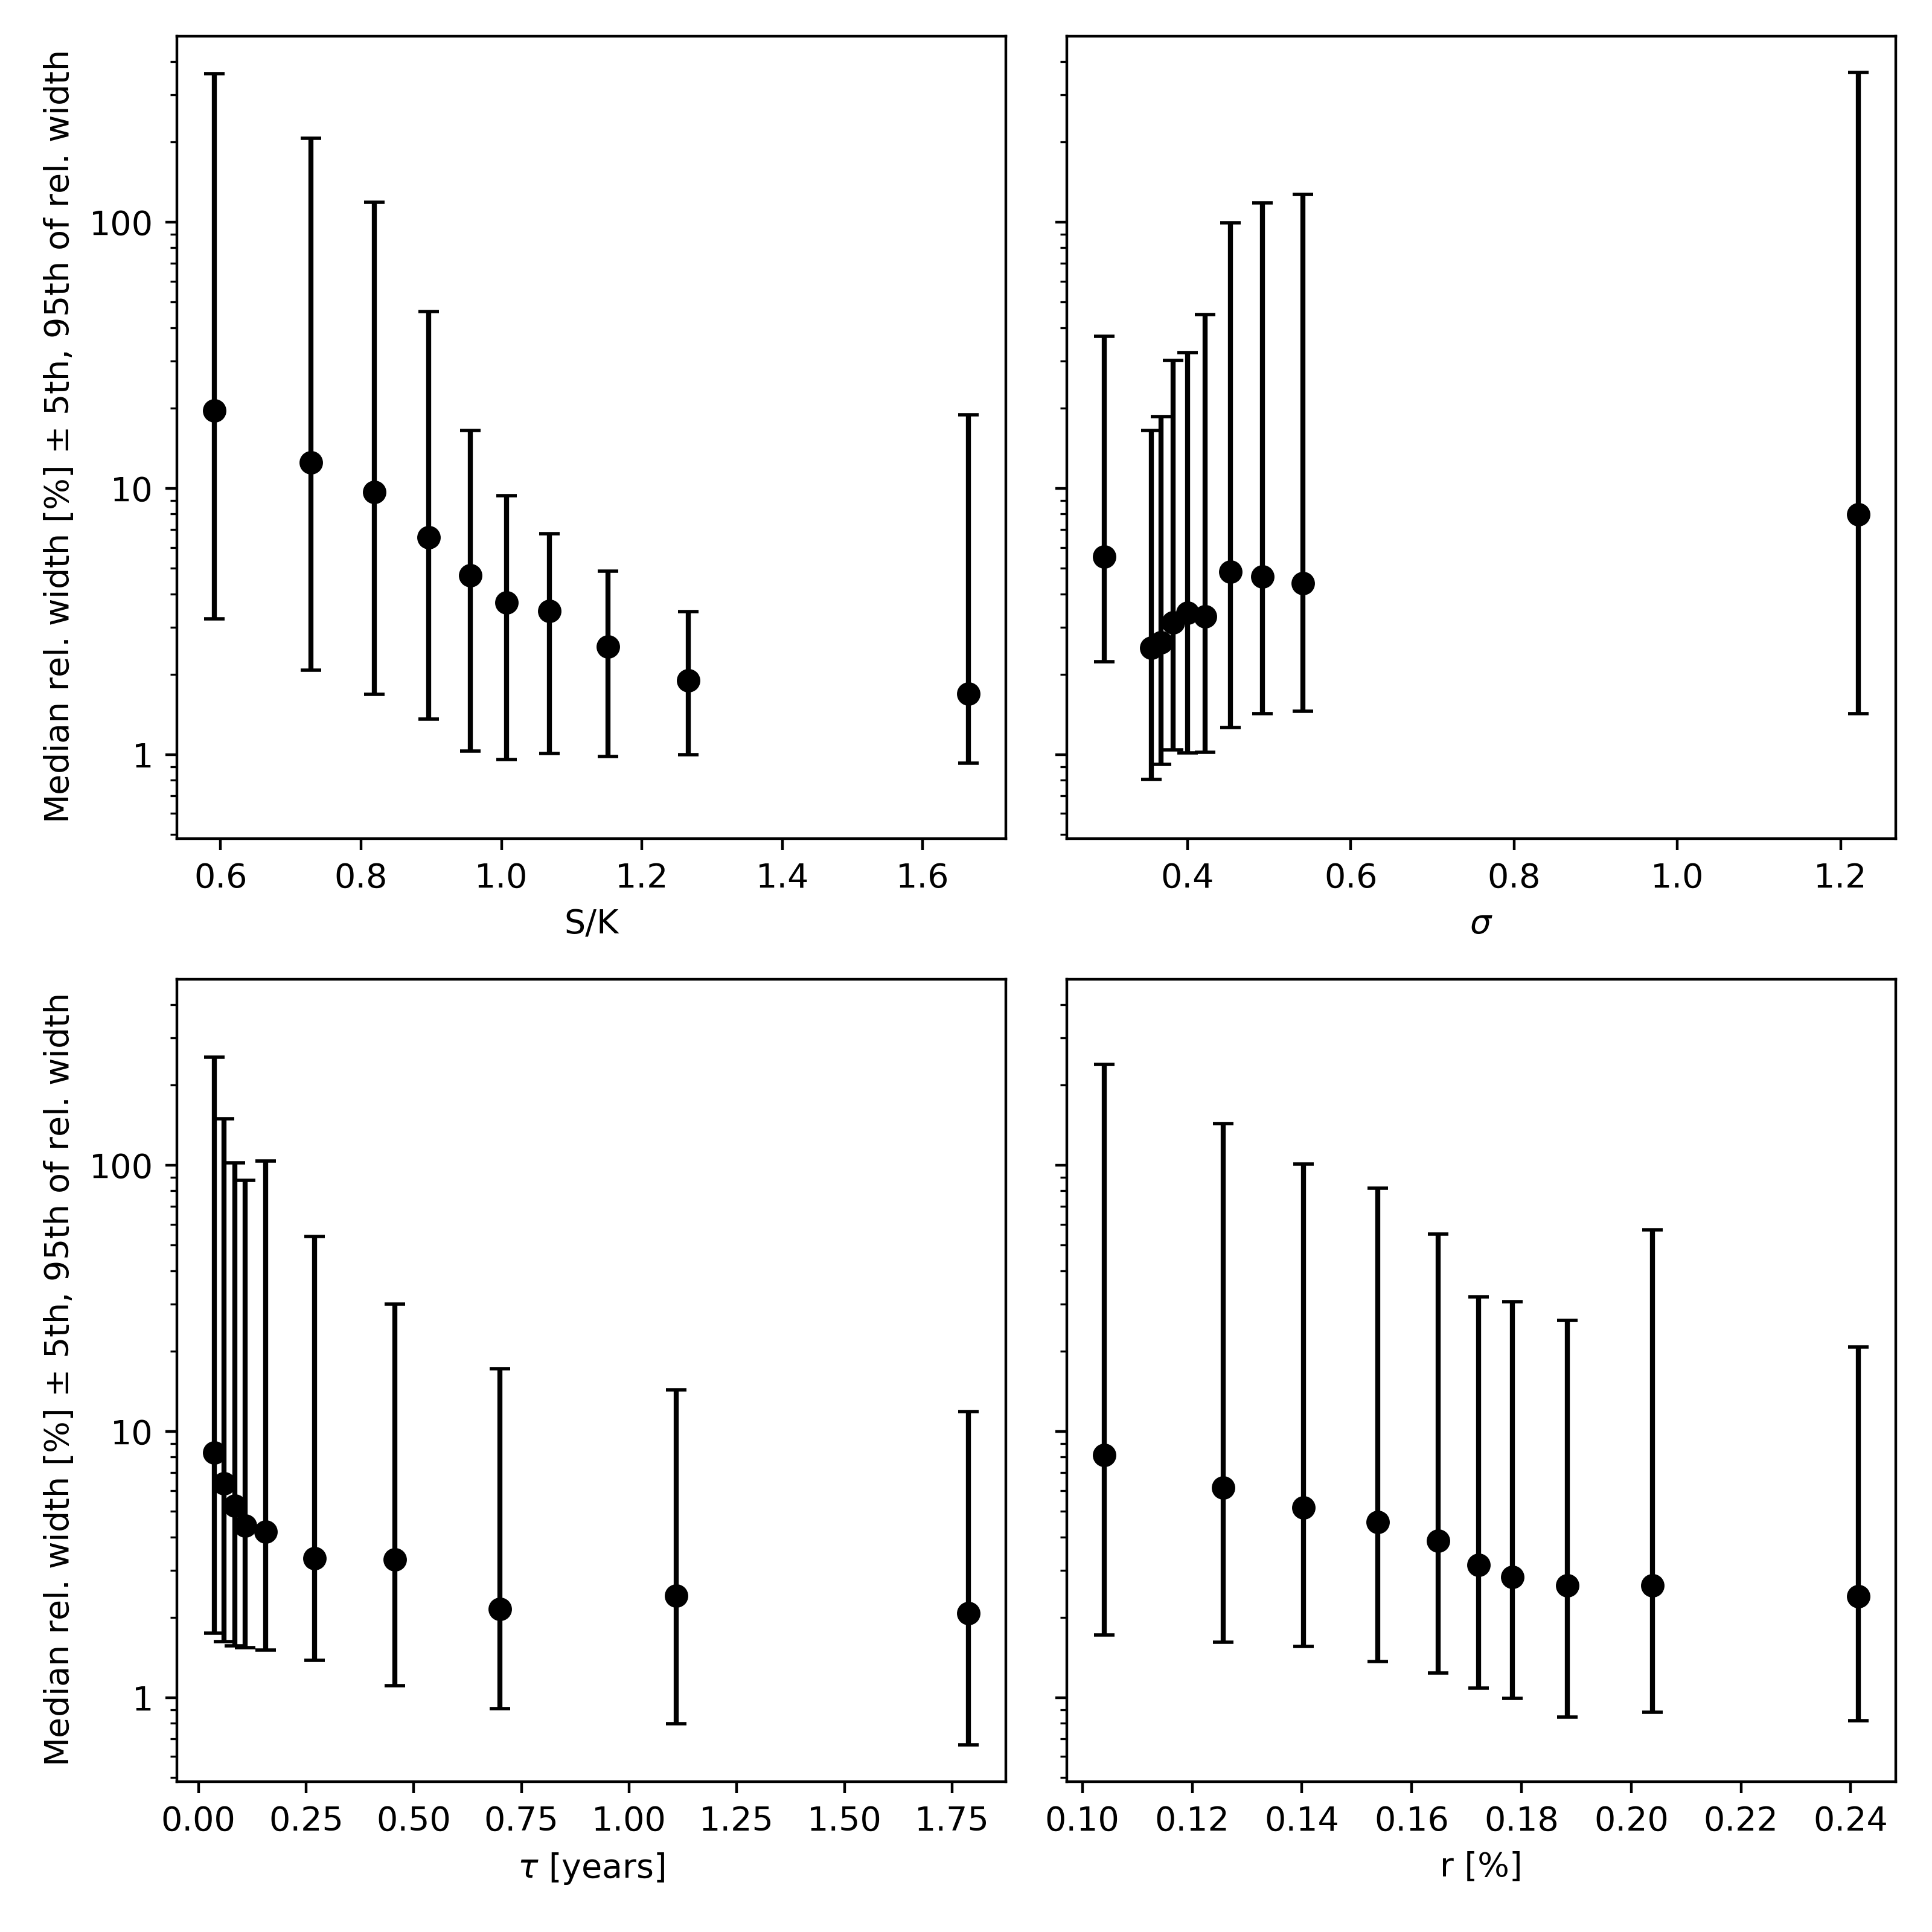
\includegraphics[width=0.8\textwidth]{reports/figures/real_data_replication/real1_rel_widths_to_features.png}
\caption{Relative widths of PIs across features. Dataset: Section \ref{sec:real1}.}
\label{fig:real1_rel_widths_vs_features}
\end{figure}

In figure \ref{fig:real1_relative_widths}, we can see that most PIs have relative widths under 10\%, and about 50\% of PIs have less than 4\% relative width. From \ref{fig:kappa4_rel_widths_vs_option_price}, we see that those relatively narrow PIs are computed for the data where option prices (normalized by K) are of orders of 0.1 or 0.01. For less than that, PIs are virtually useless, as their relative width is too often above 10\%.   

Plots for this section are computed using code at \texttt{4.4-mz-real-data-reproduction.ipynb}.

\begin{figure}
\begin{subfigure}{0.5\textwidth}
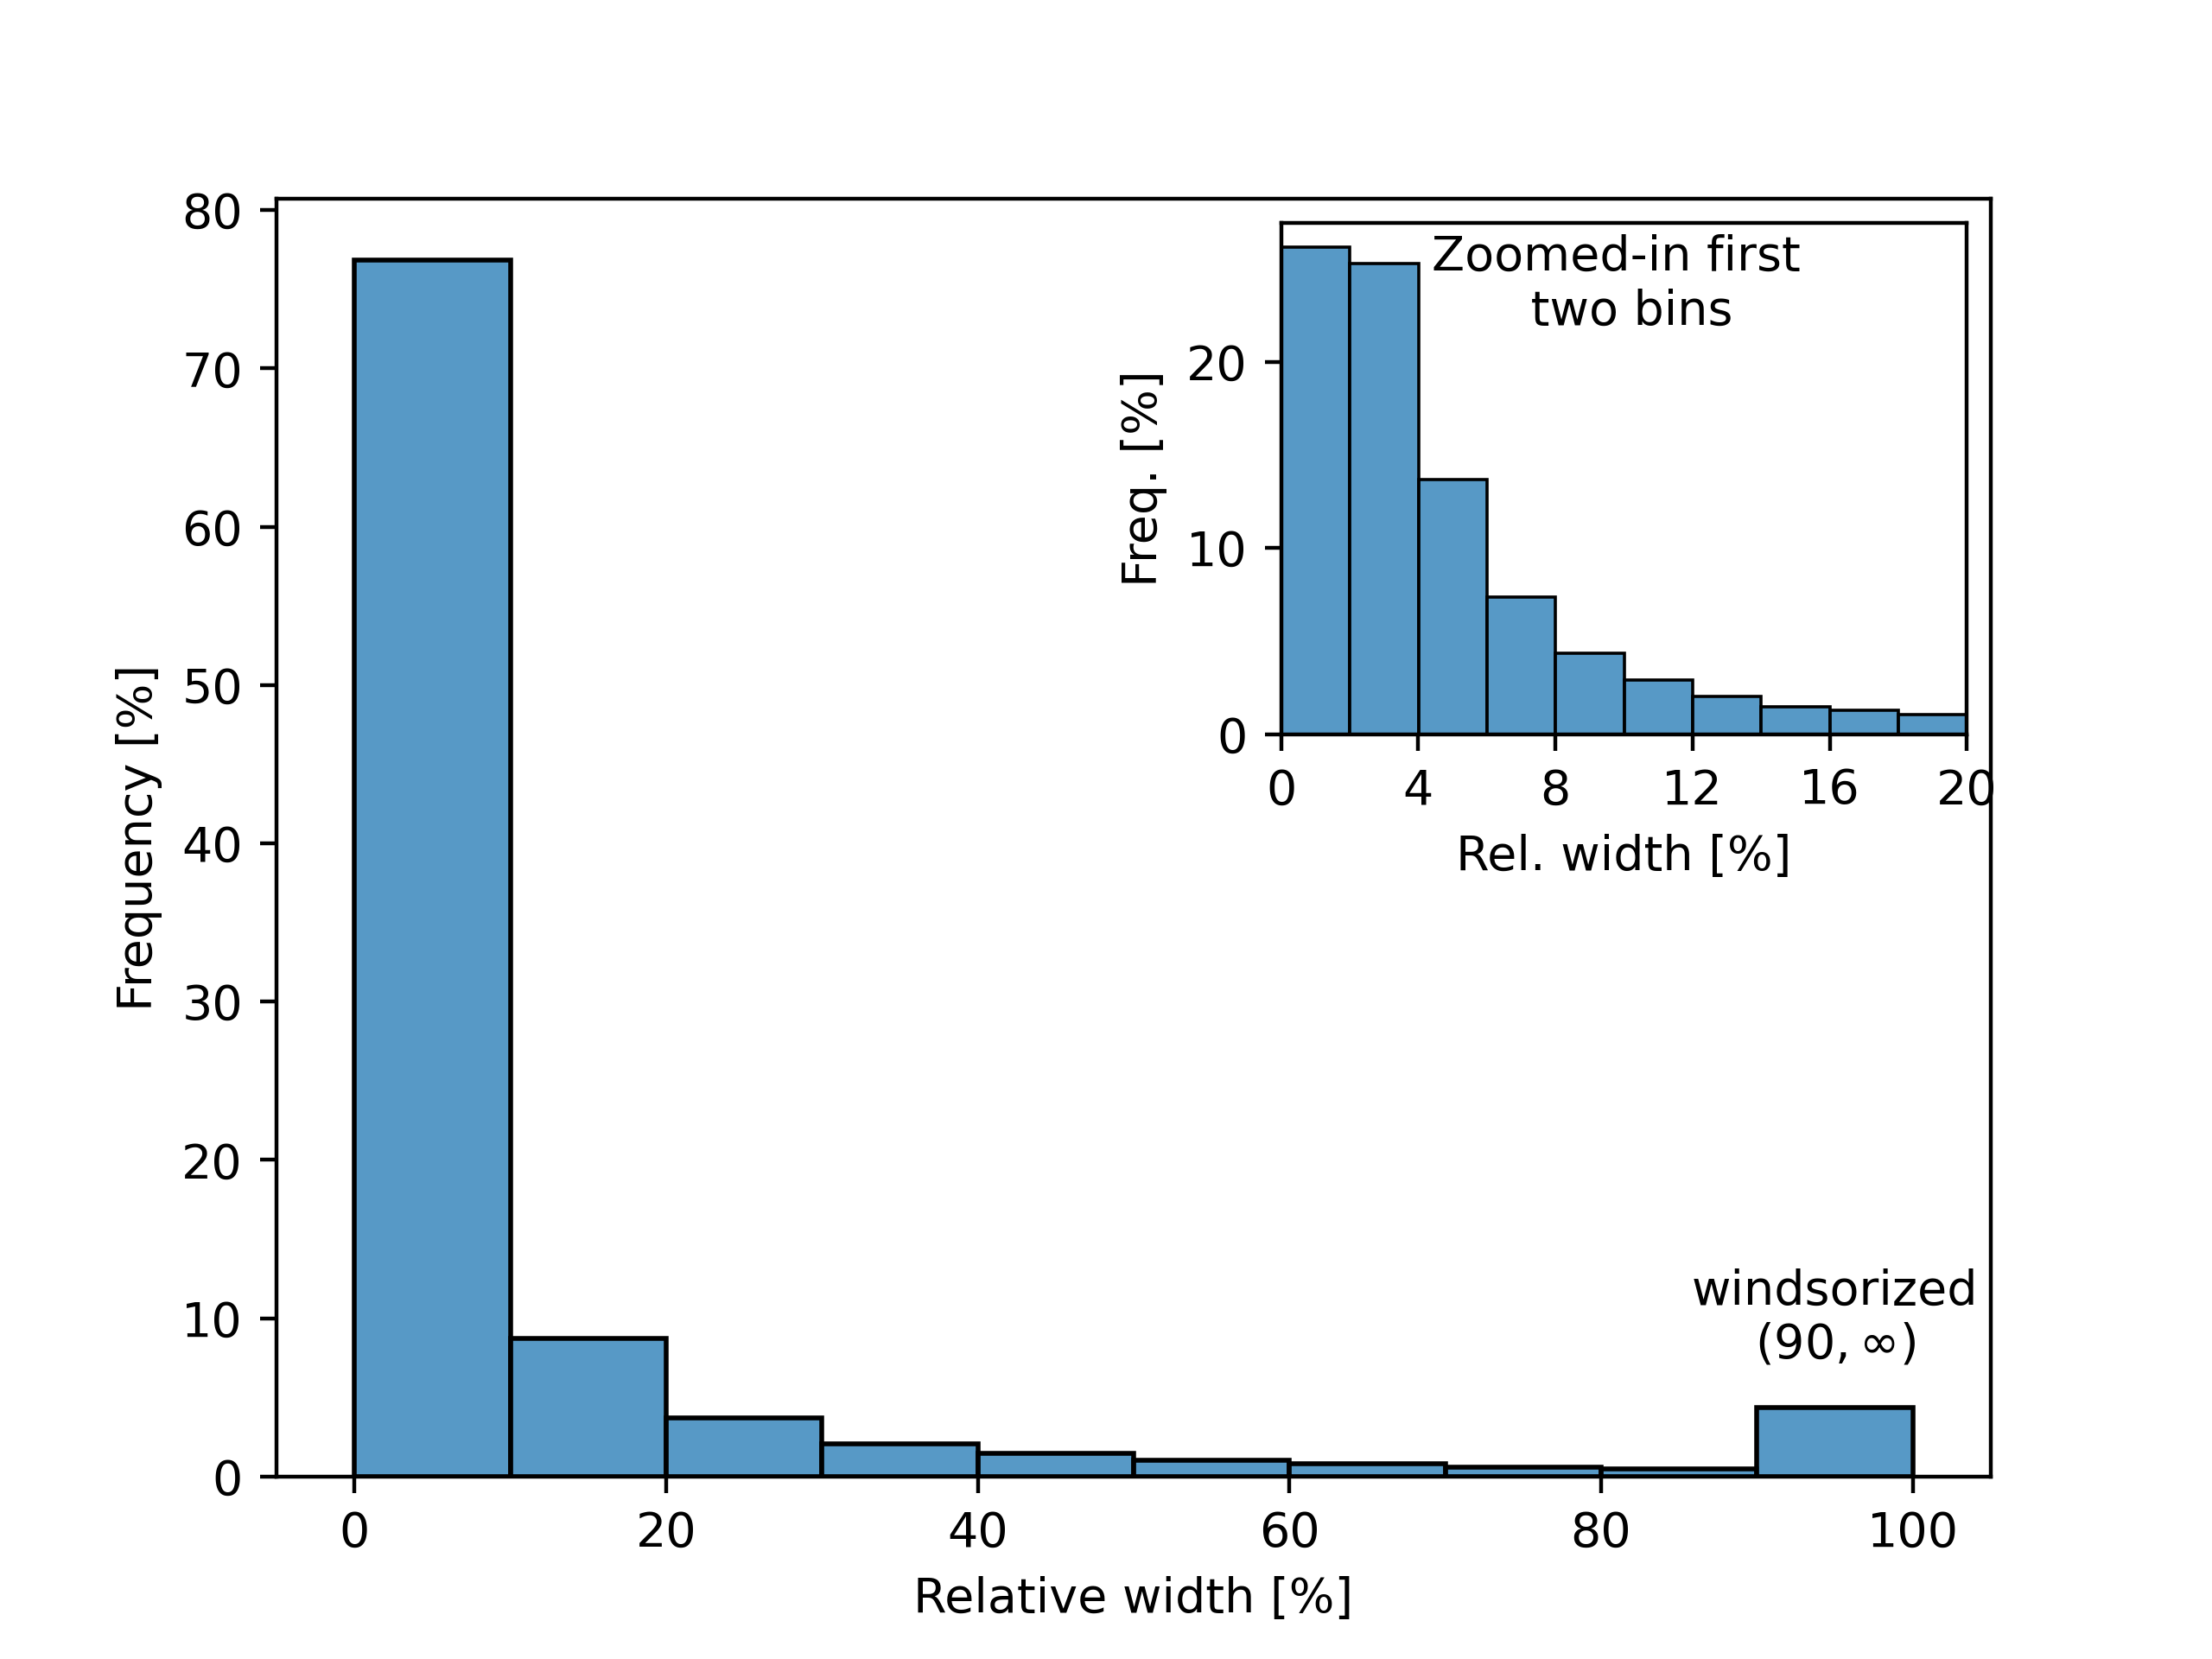
\includegraphics[width=1\linewidth]{reports/figures/real_data_replication/real1_relative_widths.png}
\caption{}
\label{fig:real1_relative_widths}
\end{subfigure}
\begin{subfigure}{0.5\textwidth}
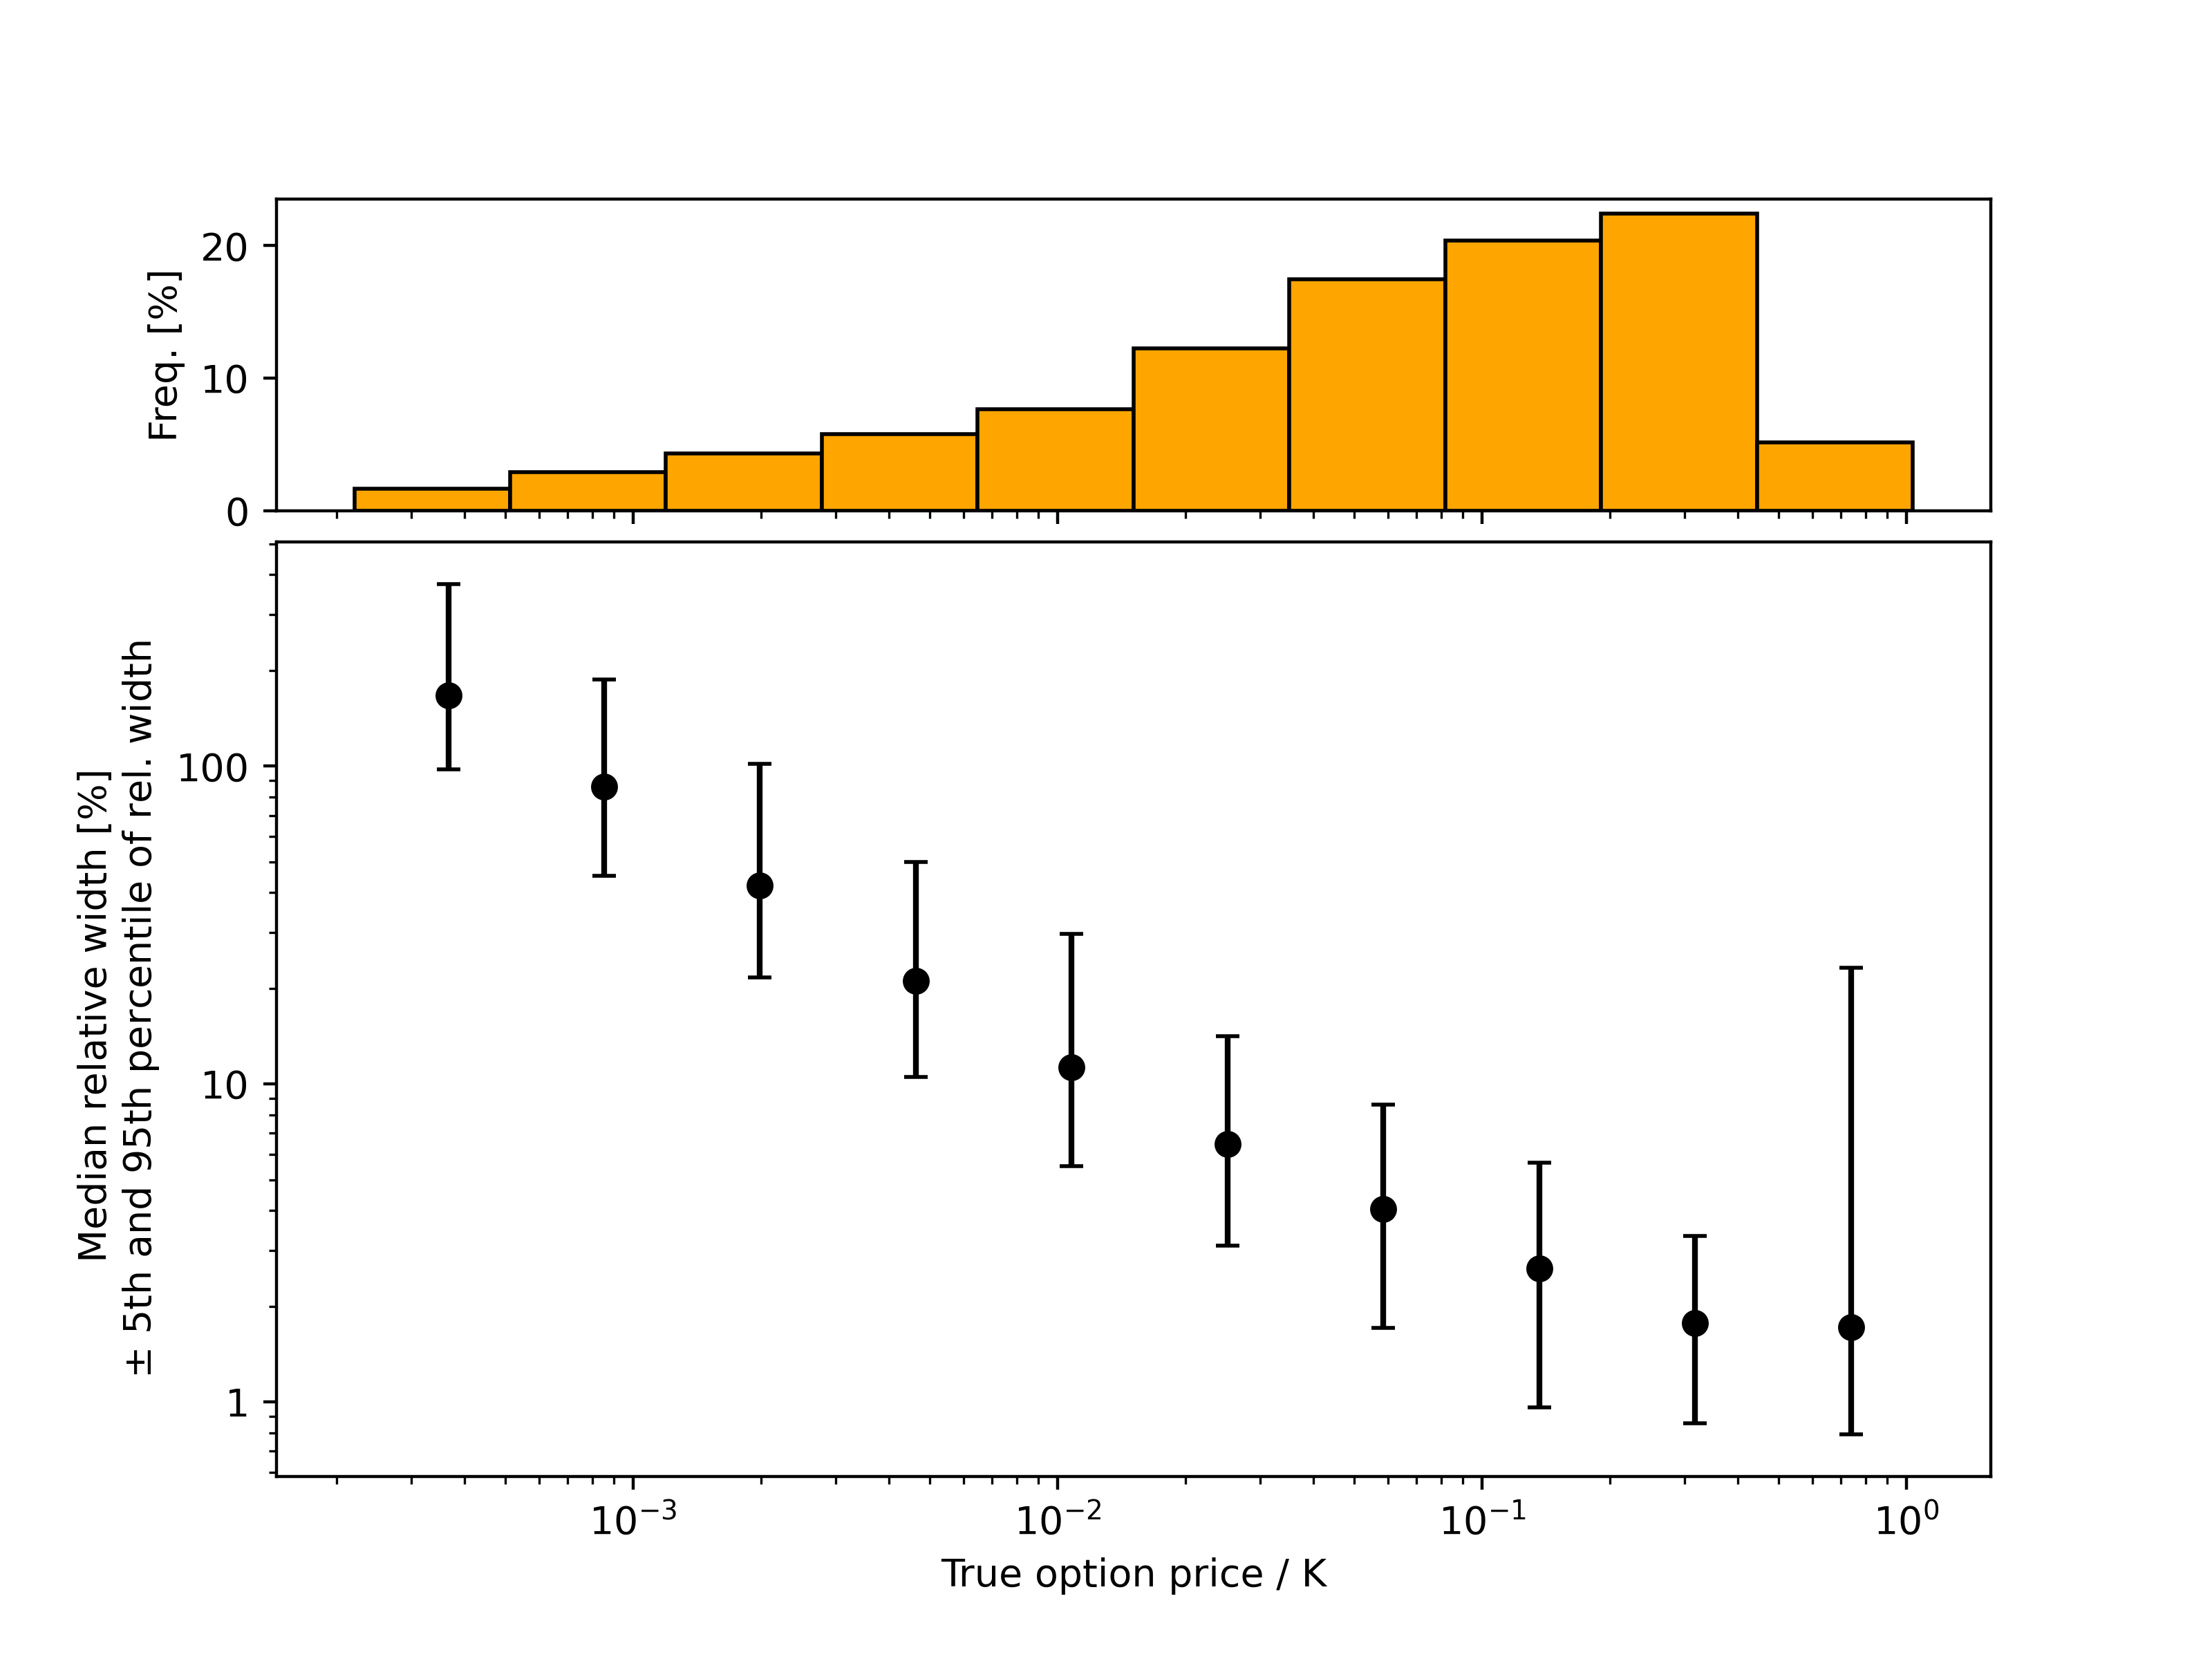
\includegraphics[width=1\linewidth]{reports/figures/real_data_replication/real1_rel_widths_to_opt_price.png} 
\caption{}
\label{fig:real1_rel_widths_to_opt_price}
\end{subfigure}
\caption{PIs binned by their relative width (a) and by the value of the target variable (b). Dataset: Section \ref{sec:real1}.}
\label{fig:real1_widths}
\end{figure}



\section{Walk-forward Testing with Real Data}

In this section, we scale up our analysis to the universe of all underlings consisting of constituents of the S\&P 500 index for the period of time from 1996.01.01 to 2022.12.31. We use the same models, with the same hyperparameters as in the section \ref{sec:real1}, i.e., as for the model with 200,000 simulated data points. This model is very likely underfitting data, but for the purpose of testing empirical coverage, the precision of the model is of second-order of importance.

Data cleaning for this section was done in the same fashion as in section 4.1, with additional filtering for positive open interest, positive trading volume, and positive bid. Also, options that have not been traded for more then 5 days by the day of observing their prices have been filtered out. Notebooks \texttt{4.1-mz-fetch-replication-data.ipynb} and \texttt{4.2-mz-fetch-big-dataset.ipynb} document fetching data for this section.

We train, calibrate, and test coverage of CQR in a walk-forward scheme. Training takes three years of data, calibration is done on the next year of data, and the following year of data is used for predicting prediction intervals. Then, the scheme is shifted by one year in the future, and training, calibration, and testing are repeated. This way, we have PIs produced for 23 years of data, where recalibration is done annually using the last year of available data. Then, for each trading day, we compute average coverage. The average coverage computed this way is presented in the figure \ref{fig:real2_average_coverage.png}   


\begin{figure}[H]
    \center 
    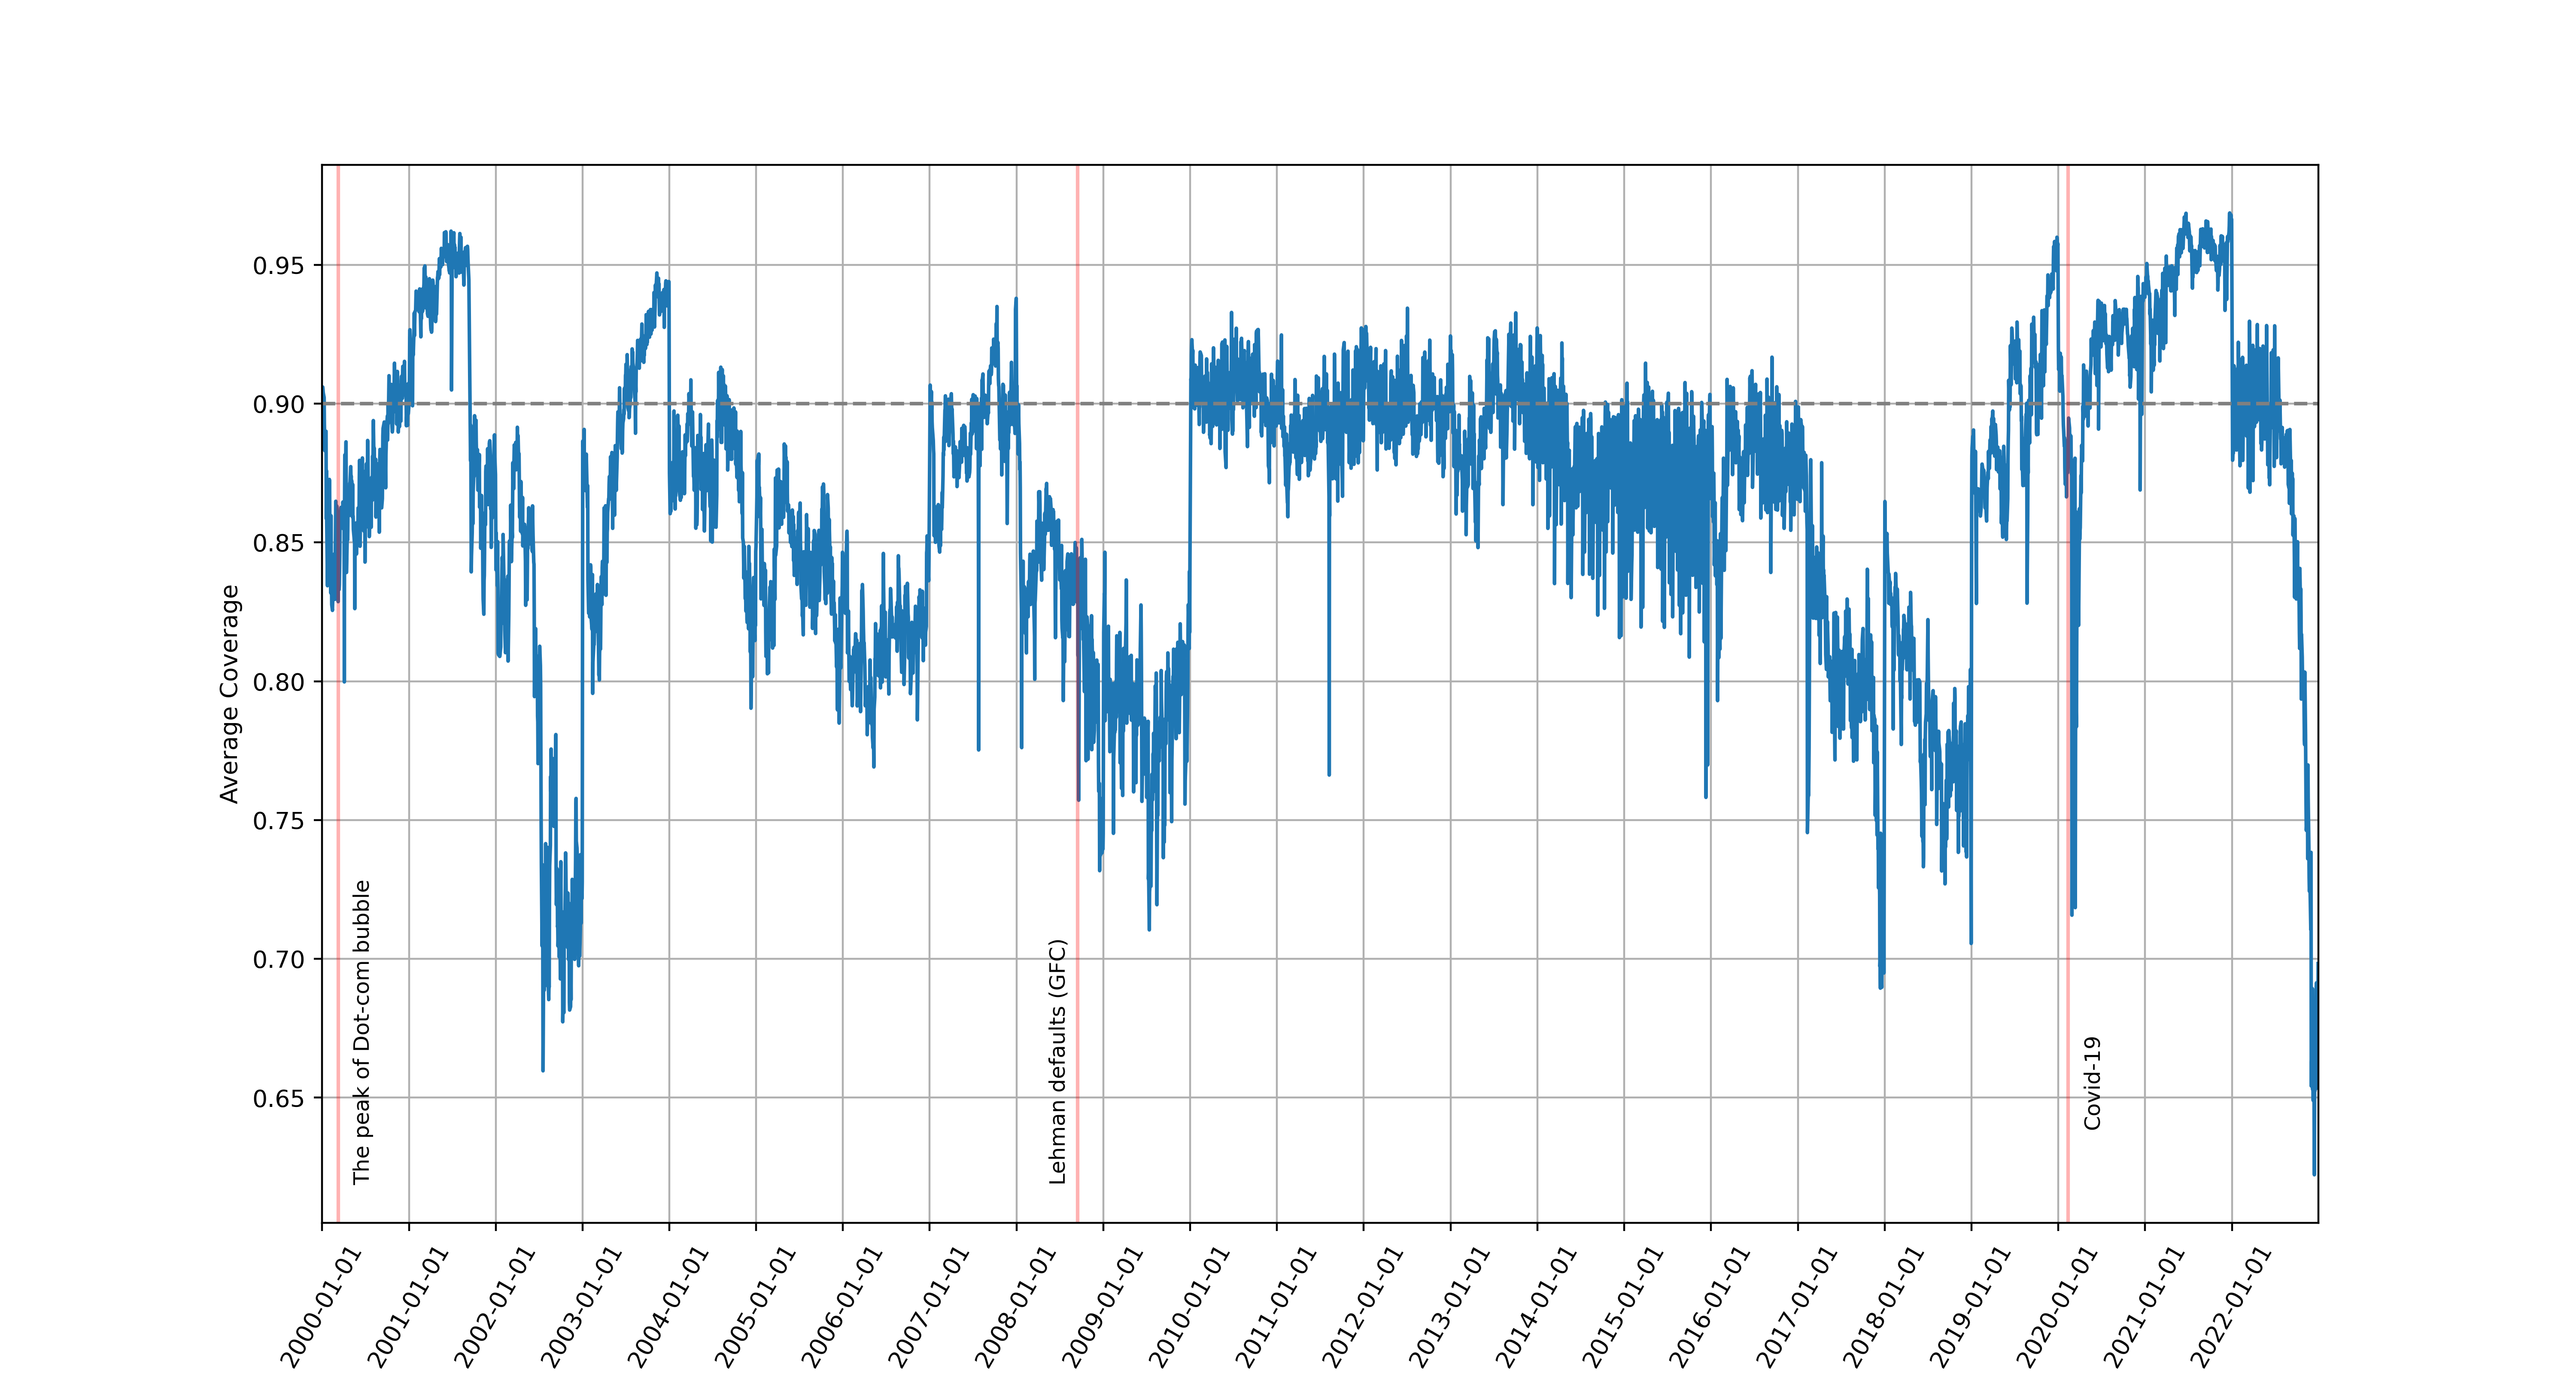
\includegraphics[width=1.1\textwidth]{reports/figures/real_data_walk_fwd/average_coverage.png}
    \caption{Average coverage for each trading day in the walk-forward scheme. CQR is recalibrated annually.}
    \label{fig:real2_average_coverage.png}
\end{figure}


\section{Conclusion}
Conformal Prediction is a powerful technique with promising results, but it heavily relies on the assumption of exchangeable data. In this setting, the finite-sample coverage guarantees, along with the methodology's simplicity and adaptability, arguably make it one of the most practical tools for uncertainty quantification. This is partly demonstrated by the superior coverage provided by CQR relative to NQR. The main question is to what extent the coverage is sustained with non-exchangeability. Simulation analysis shows that several strikes for a single underlying introduces non-exchangeability, and ruins coverage guarantees of CQR. Nevertheless, CQR consistently outperforms NQR in any case, with both methods underperforming in sparse data regions such as deep moneyness and large volatility. Further investigation must be made into comparing CQR to other methods of uncertainty quantification, such as deep ensembles. 

In this report, we show that by applying CQR to the real option data and by performing out-of-time testing of coverage, empirical coverage of the CP method fails. However, this is in contrast to the results observed in the empirical study of \cite{bastos}, which showcases that CP coverage is maintained for real options data. We believe the reason for this is that the randomization of training, split, and test sets present in the study unintentionally introduces exchangeability across the calibration and test sets. 


To illustrate why this is detrimental, consider a trained model with calibration set $\mathcal{D}$ and test set $\mathcal{D}_*$ in the setting of split conformal prediction. 
If the randomization leads $\mathcal{D} \cup \mathcal{D}_*$ to be exchangeable, then coverage will falsely seem to be provided on the test set. On the other hand, any new trial point, $(X_{n+1}, Y_{n+1})$, would not be exchangeable with $\mathcal{D}$, so in reality the PIs would undercover. We do not concretely prove that this randomization introduces exchangeability, but it seems to be the only explanation for the empirical discrepancies in coverage. Indeed, perfect coverage is also observed when randomization of training, calibration and test sets is implemented in our study, despite the option data being clearly non-exchangeable. 

The non-exchangeability of options data is argued to be evident due to the degeneracy introduced by options of different strikes existing for the same underlying, implying a need for the same $S$\footnote{and $\sigma$ under Black-Scholes, but this is not necessarily the case when the volatility smile is considered} across these data points. Even in the case where such degeneracies are not present, and there is only one strike quoted for each underlying, the data will not be exchangeable because the marginal distributions of $(S, \sigma, K, r, \tau)$ will not be the same. Nevertheless, if degeneracies are removed it is expected that the data is relatively more exchangeable. An interesting approach would therefore be to remove degeneracies in the calibration set by restricting it to only include options with a particular strike price for each underlying. The nonconformity score of a new trial point will then be more exchangeable with the scores from this set. To take this one step further, the ML model can be adapted to the input $(S, \sigma, K, r, \tau)$ that is to be priced as follows: Firstly, calculate the L-2 norm discrepancies between the input covariates and data covariates. Then select the data entries closest to the input. Given their similar values these datapoints are more likely to have the same behaviour as the input, so take these to be the calibration set. Train the model on the rest of the data, and then perform the CP procedure. The drawback of this is that the most similar values to the input are not included in training the pricing model, but are instead prioritised to increase exchangeability and coverage. It is still important to include a fine enough grid of $(S, \sigma, K, r, \tau)$ in both the training set, for a better ML model, and in the calibration set, for more complete non-conformity scores.

The extent to which a dataset is exchangeable is difficult to quantify. There are statistical tests for exchangeability, but these are weak and computationally expensive. Additionally, they only lead to acceptance or rejection; there is no relative adherence. In the case where exchangeability can be quantified, there are extensions of the CP methodology that yield better performance. For example, Mondrian CP \cite{vovk2005} partitions data into categories where exchangeability holds within each group. This approach is particularly useful in hierarchical models and applications involving group-specific distributions. Weighted CP ~\cite{beyond_exchange} is another such framework, which addresses issues regarding exchangeability by assigning weights to observations based on their relevance. Interestingly then, CP misscoverage appears to be a good quantifier of exchangeability, and could be explored in conjunction with these methods or for further applications.


% Sets the bibliography style to UNSRT and imports the 
% bibliography file "sample.bib".
\bibliographystyle{unsrt}
\bibliography{references}

\newpage

\section{Appendix}

% CQR

\begin{figure}[H]
    \centering
    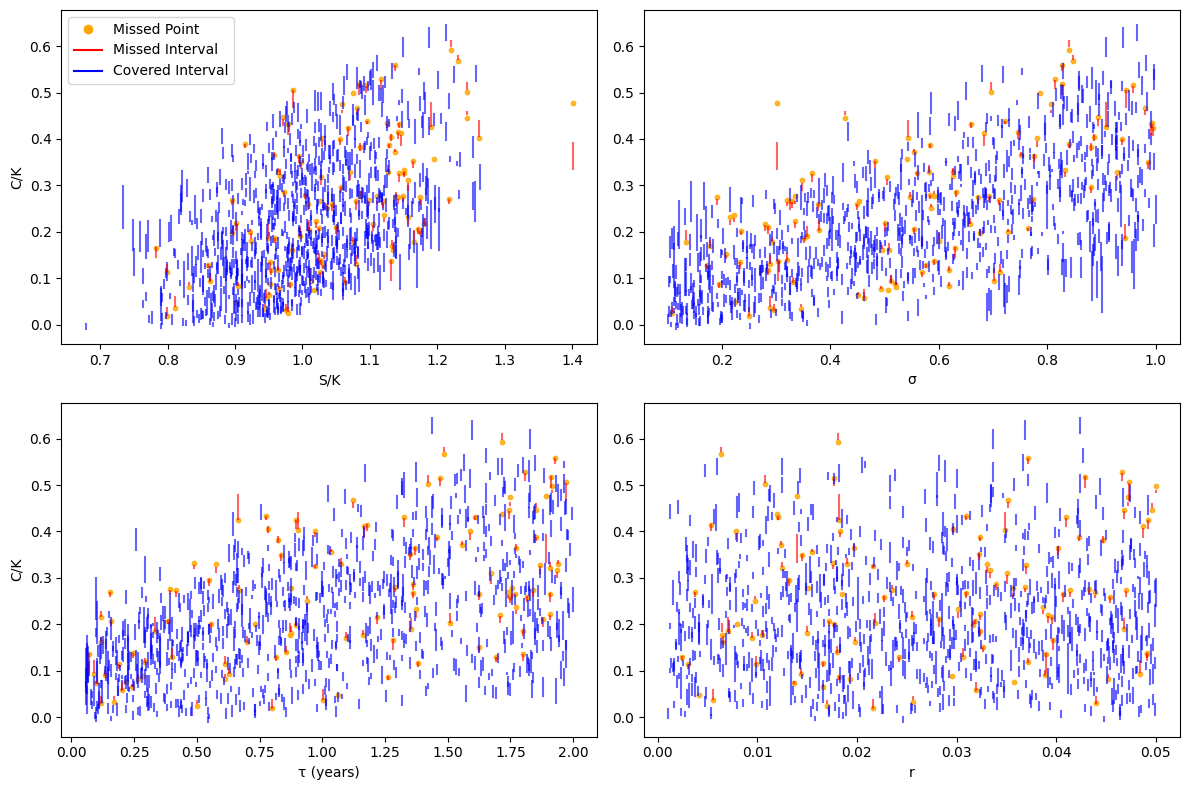
\includegraphics[width=0.8\textwidth]{reports/figures/3.3-nm-figures/sample_0/CQR_PIs_0.png}
    \caption{CQR prediction intervals for 5,000 samples. Covered intervals are shown in blue, missed intervals in red, and missed points in orange. Every 500th data point plotted.}
    \label{fig:CQR_PIs_0}
\end{figure}

\begin{figure}[H]
    \centering
    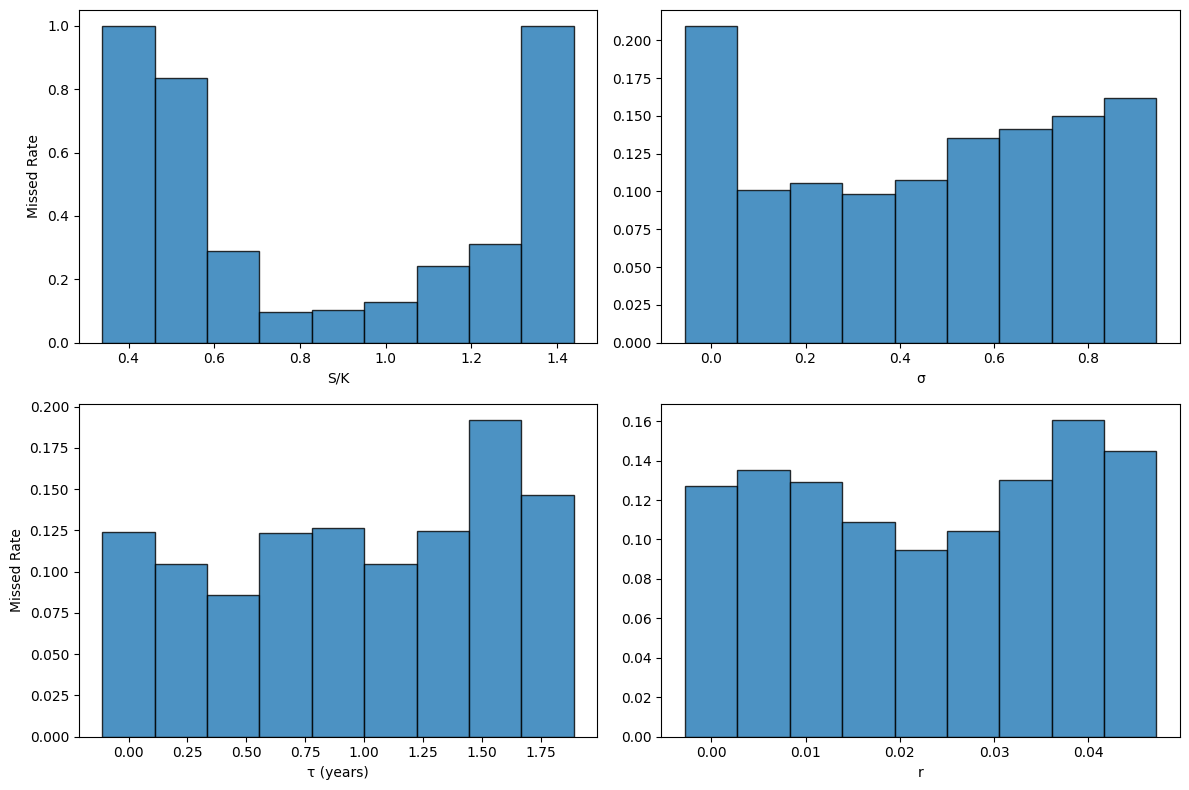
\includegraphics[width=0.8\textwidth]{reports/figures/3.3-nm-figures/sample_0/CQR_MISSED_RATE_0.png}
    \caption{CQR missed rates for 5,000 samples, plotted across 10 bins of moneyness, volatility, time-to-maturity (years), and interest rate.}
    \label{fig:CQR_MISSED_RATE_0}
\end{figure}

% NQR

\begin{figure}
    \centering
    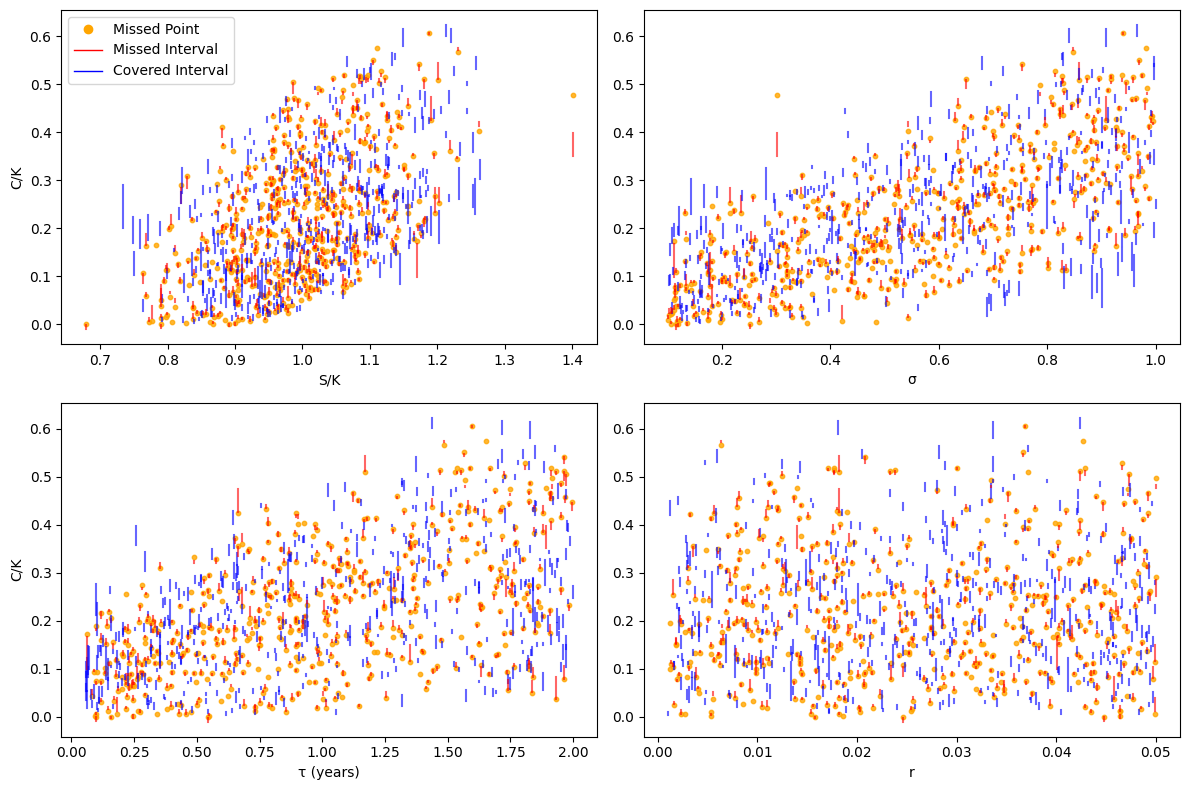
\includegraphics[width=0.8\textwidth]{reports/figures/3.3-nm-figures/sample_0/NQR_PIs_0.png}
    \caption{NQR prediction intervals for 5,000 samples. Covered intervals are shown in blue, missed intervals in red, and missed points in orange. Every 500th data point plotted.}
    \label{fig:NQR_PIs_0}
\end{figure}

\begin{figure}
    \centering
    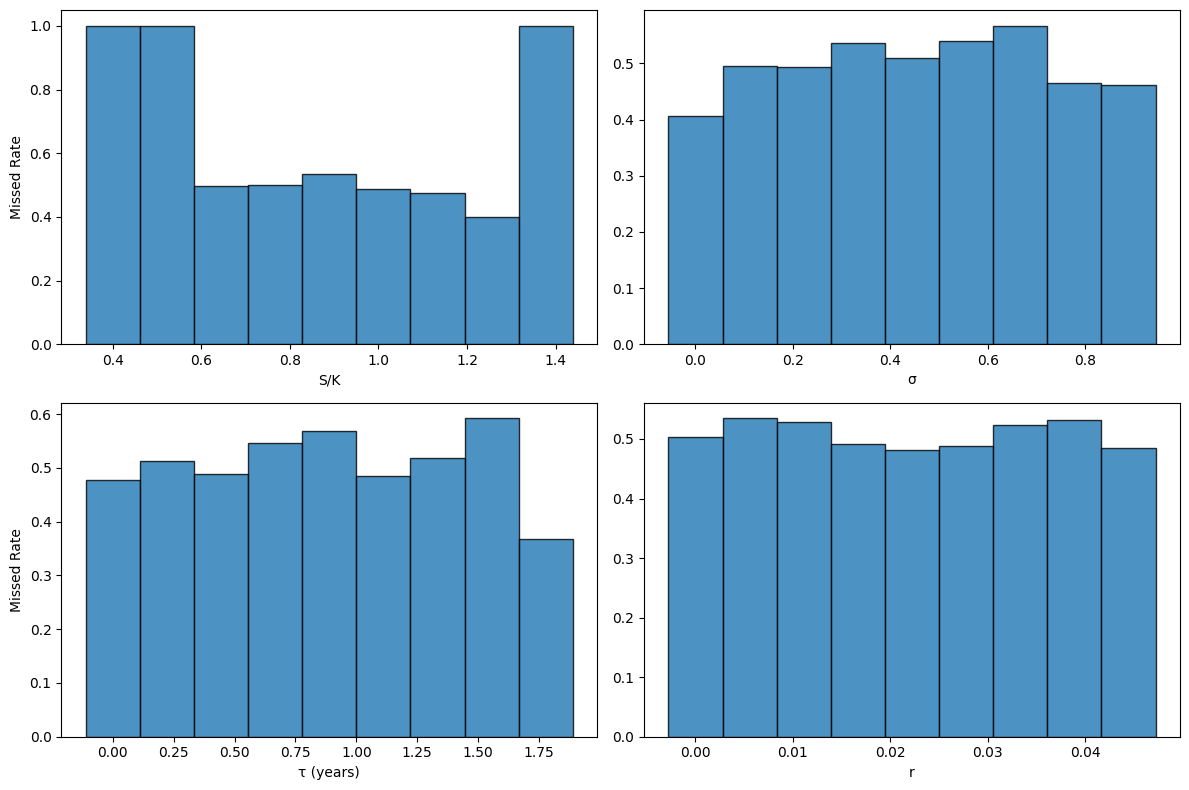
\includegraphics[width=0.8\textwidth]{reports/figures/3.3-nm-figures/sample_0/NQR_MISSED_RATE_0.png}
    \caption{NQR missed rates for 5,000 samples, plotted across 10 bins of moneyness, volatility, time-to-maturity (years), and interest rate.}
    \label{fig:NQR_MISSED_RATE_0}
\end{figure}

\begin{figure}
    \centering
    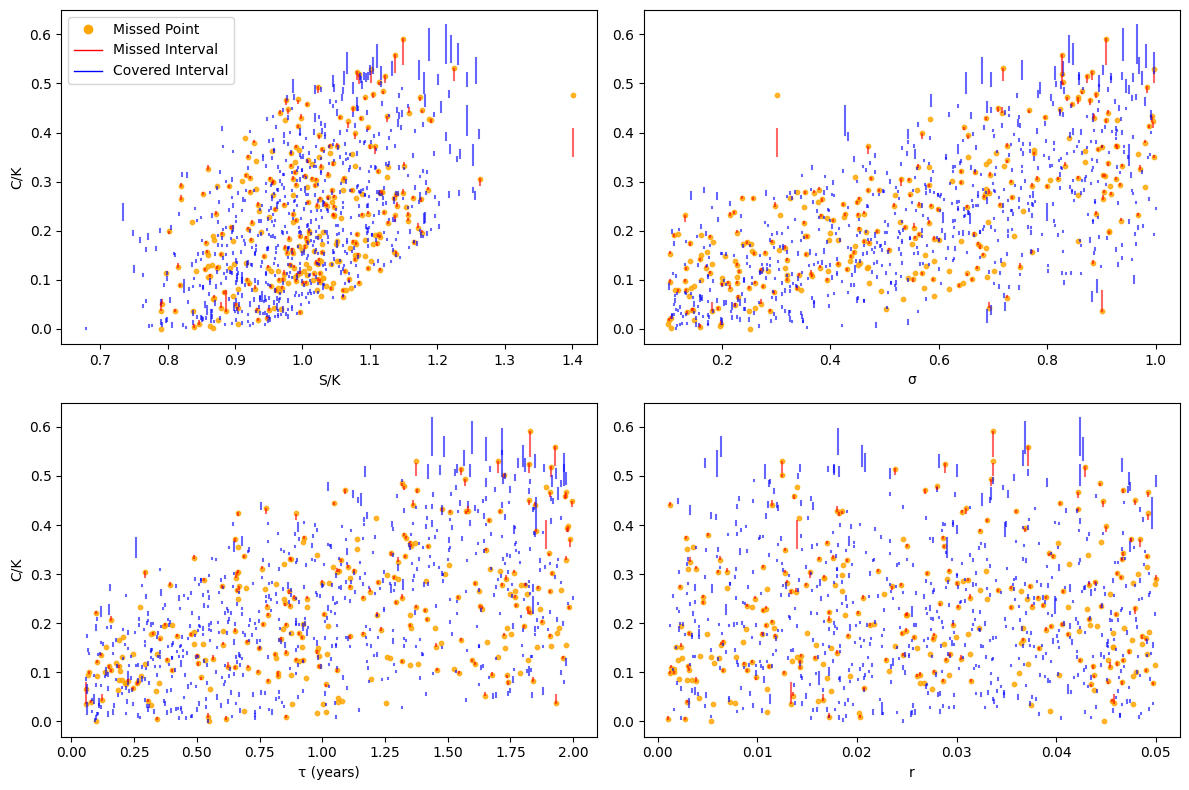
\includegraphics[width=0.8\textwidth]{reports/figures/3.3-nm-figures/sample_5/NQR_PIs_5.png}
    \caption{NQR prediction intervals for 200,000 samples. Covered intervals are shown in blue, missed intervals in red, and missed points in orange. Every 500th data point plotted.}
    \label{fig:NQR_PIs_5}
\end{figure}

\begin{figure}
    \centering
    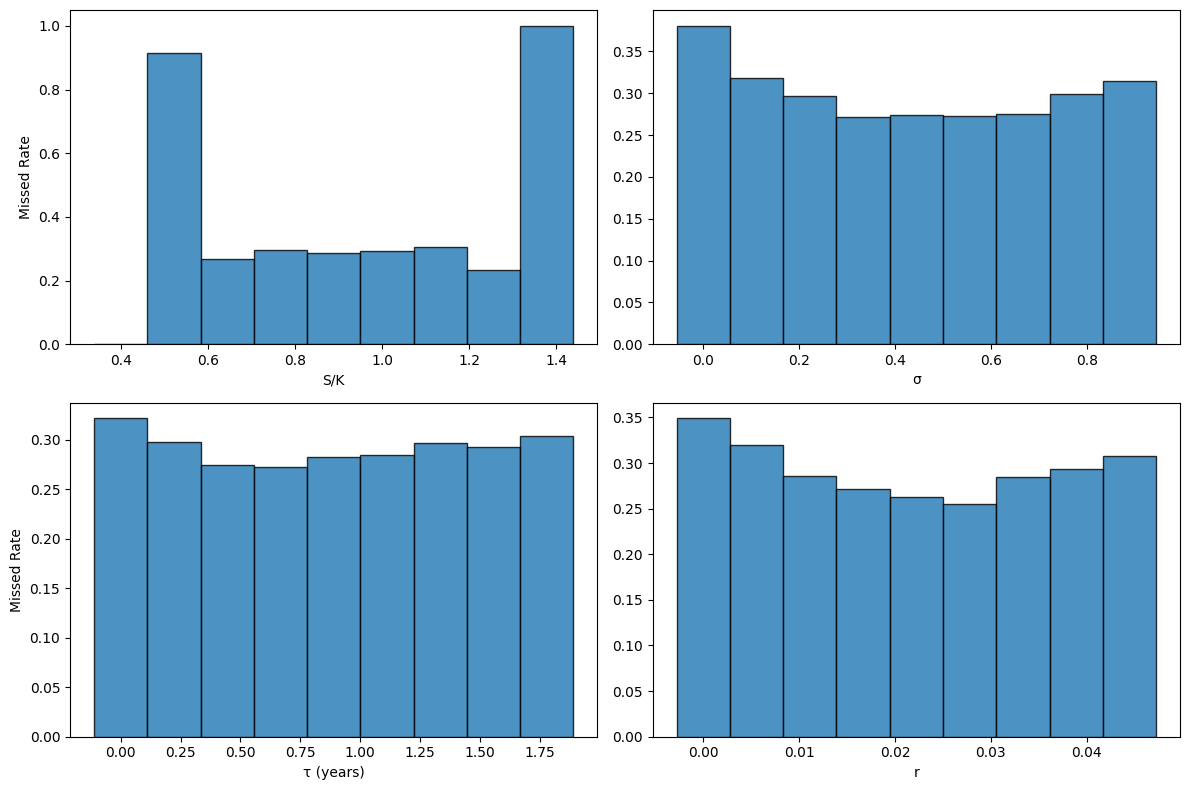
\includegraphics[width=0.8\textwidth]{reports/figures/3.3-nm-figures/sample_5/NQR_MISSED_RATE_5.png}
    \caption{NQR missed rates for 200,000 samples, plotted across 10 bins of moneyness, volatility, time-to-maturity (years), and interest rate.}
    \label{fig:NQR_MISSED_RATE_5}
\end{figure}

% kappa = 1

\begin{figure}
\centering
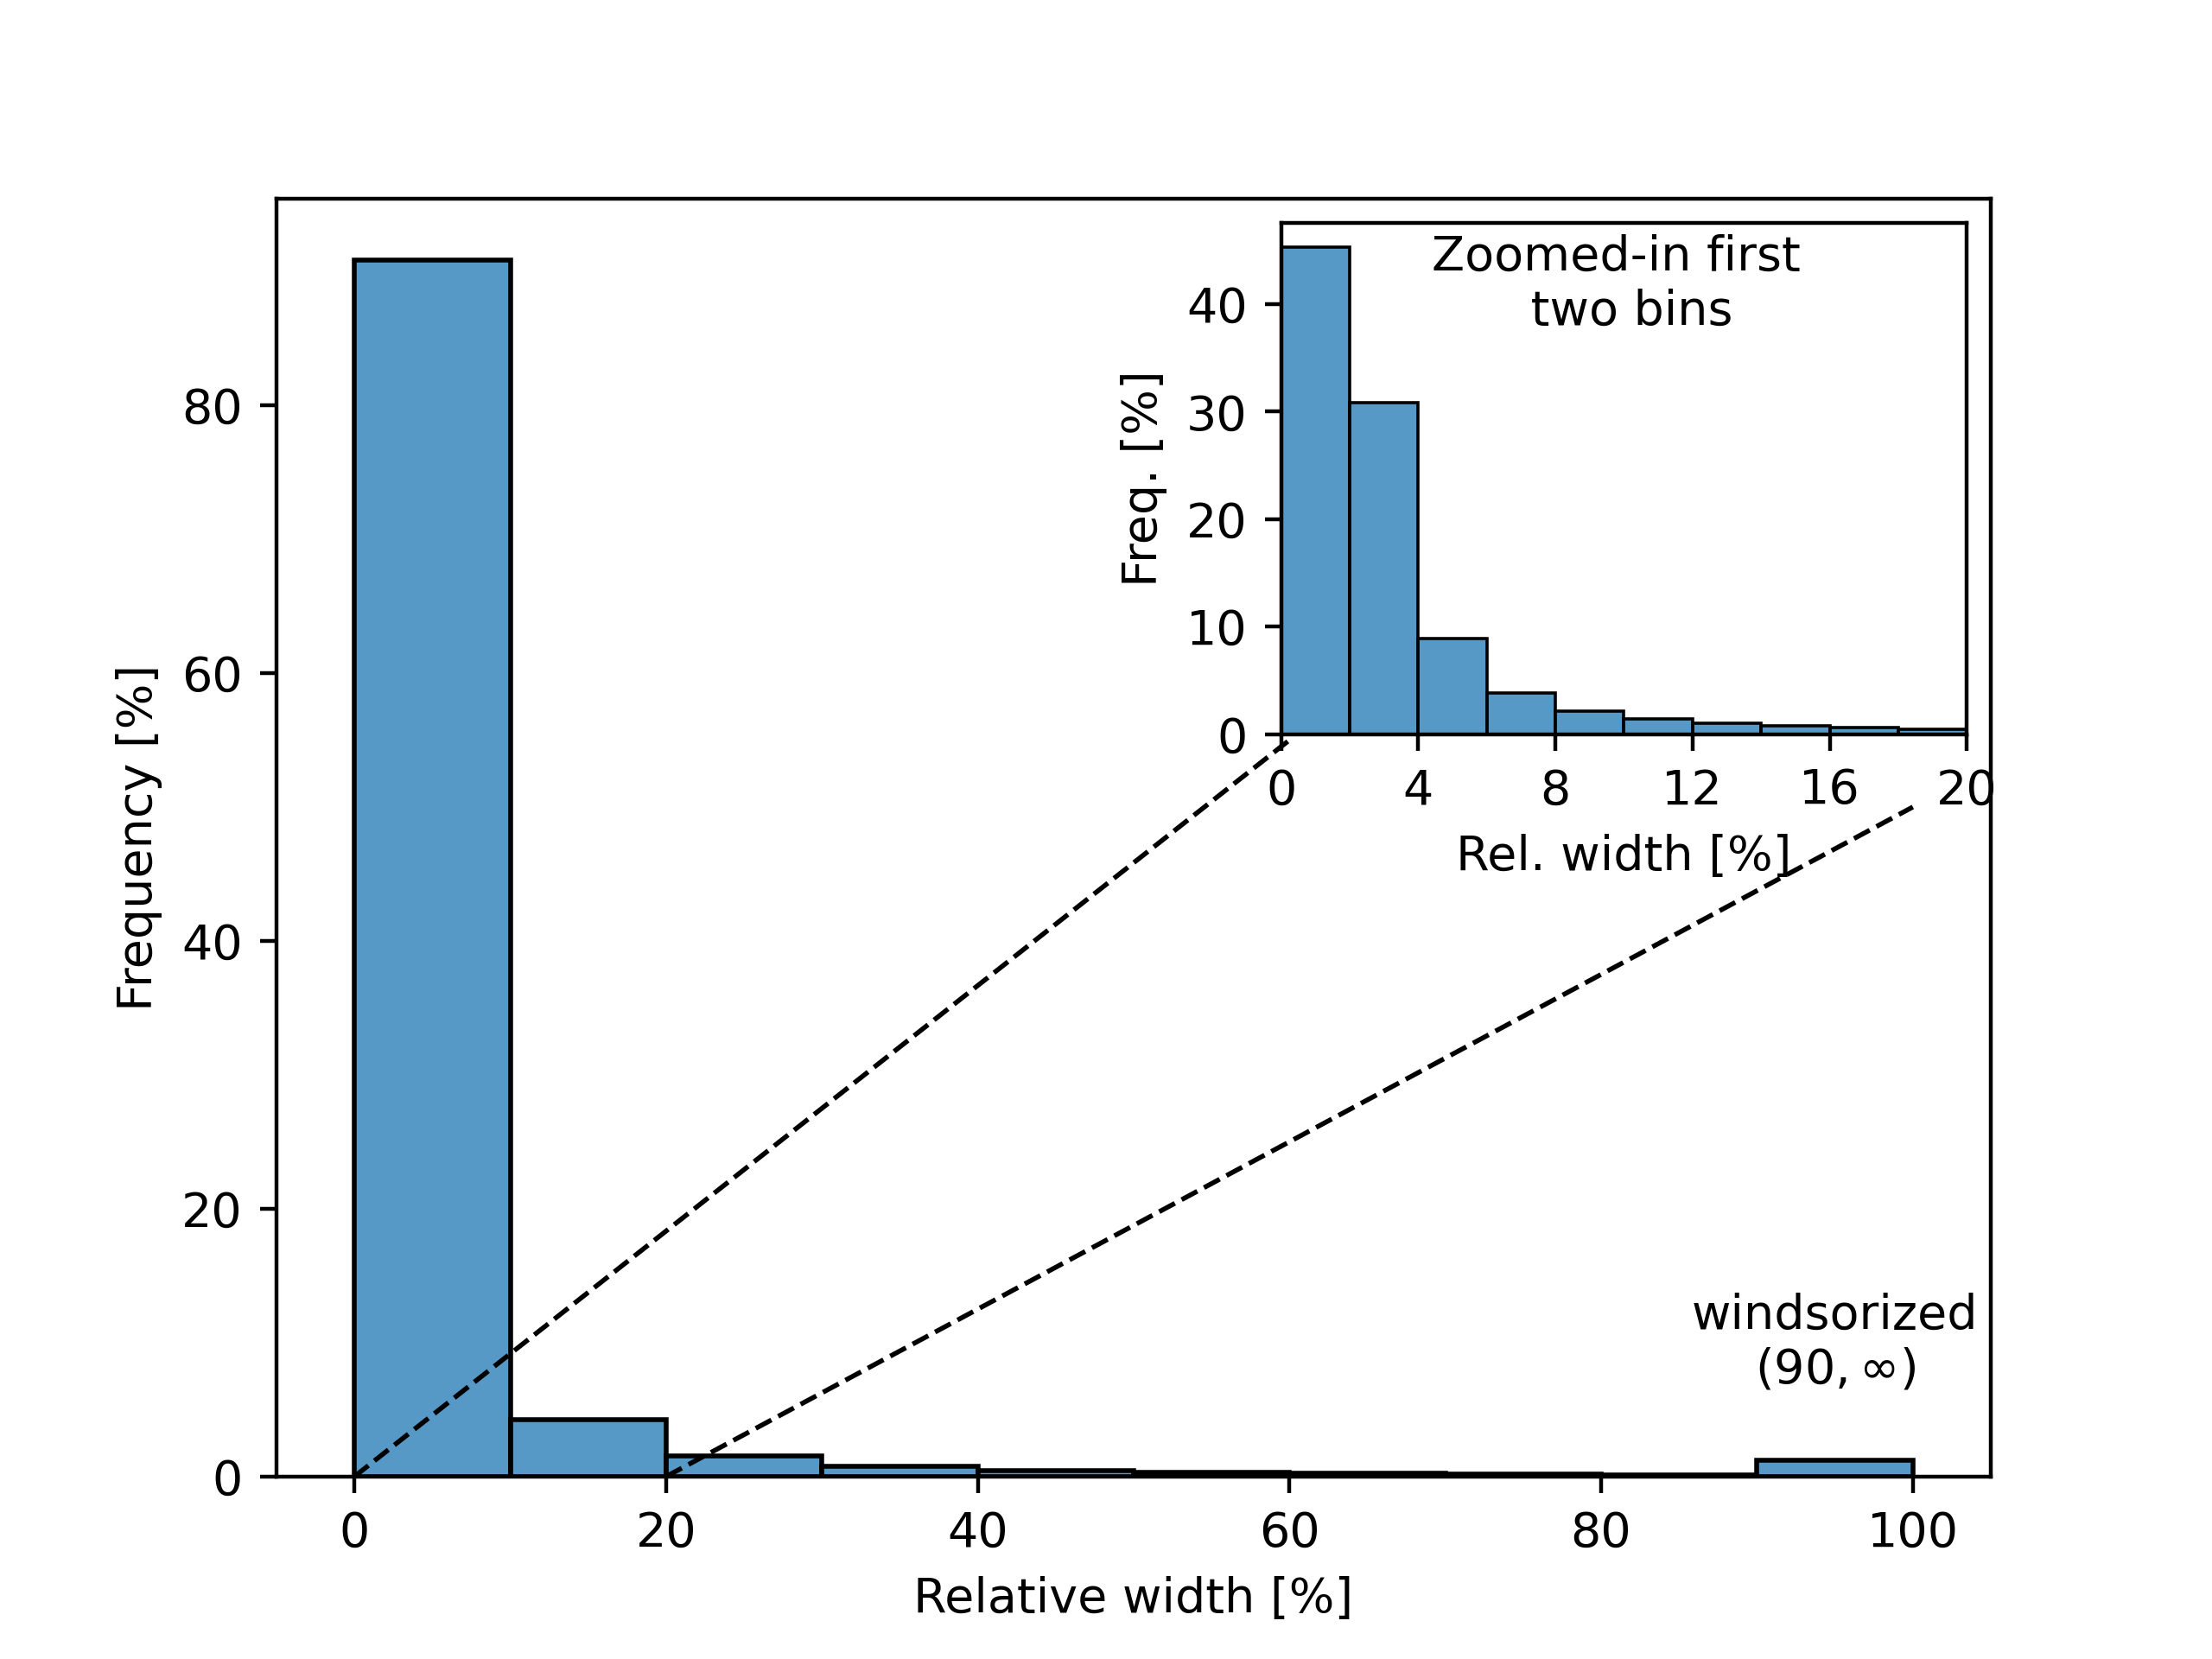
\includegraphics[width=0.8\textwidth]{reports/figures/simulated_data/sim_kappa1_relative_widths.png}
\caption{Distributions of relative widths of PIs for $\kappa=1$.}
%\label{fig:kappa4_rel_widths}
\end{figure}

\begin{figure}
\centering
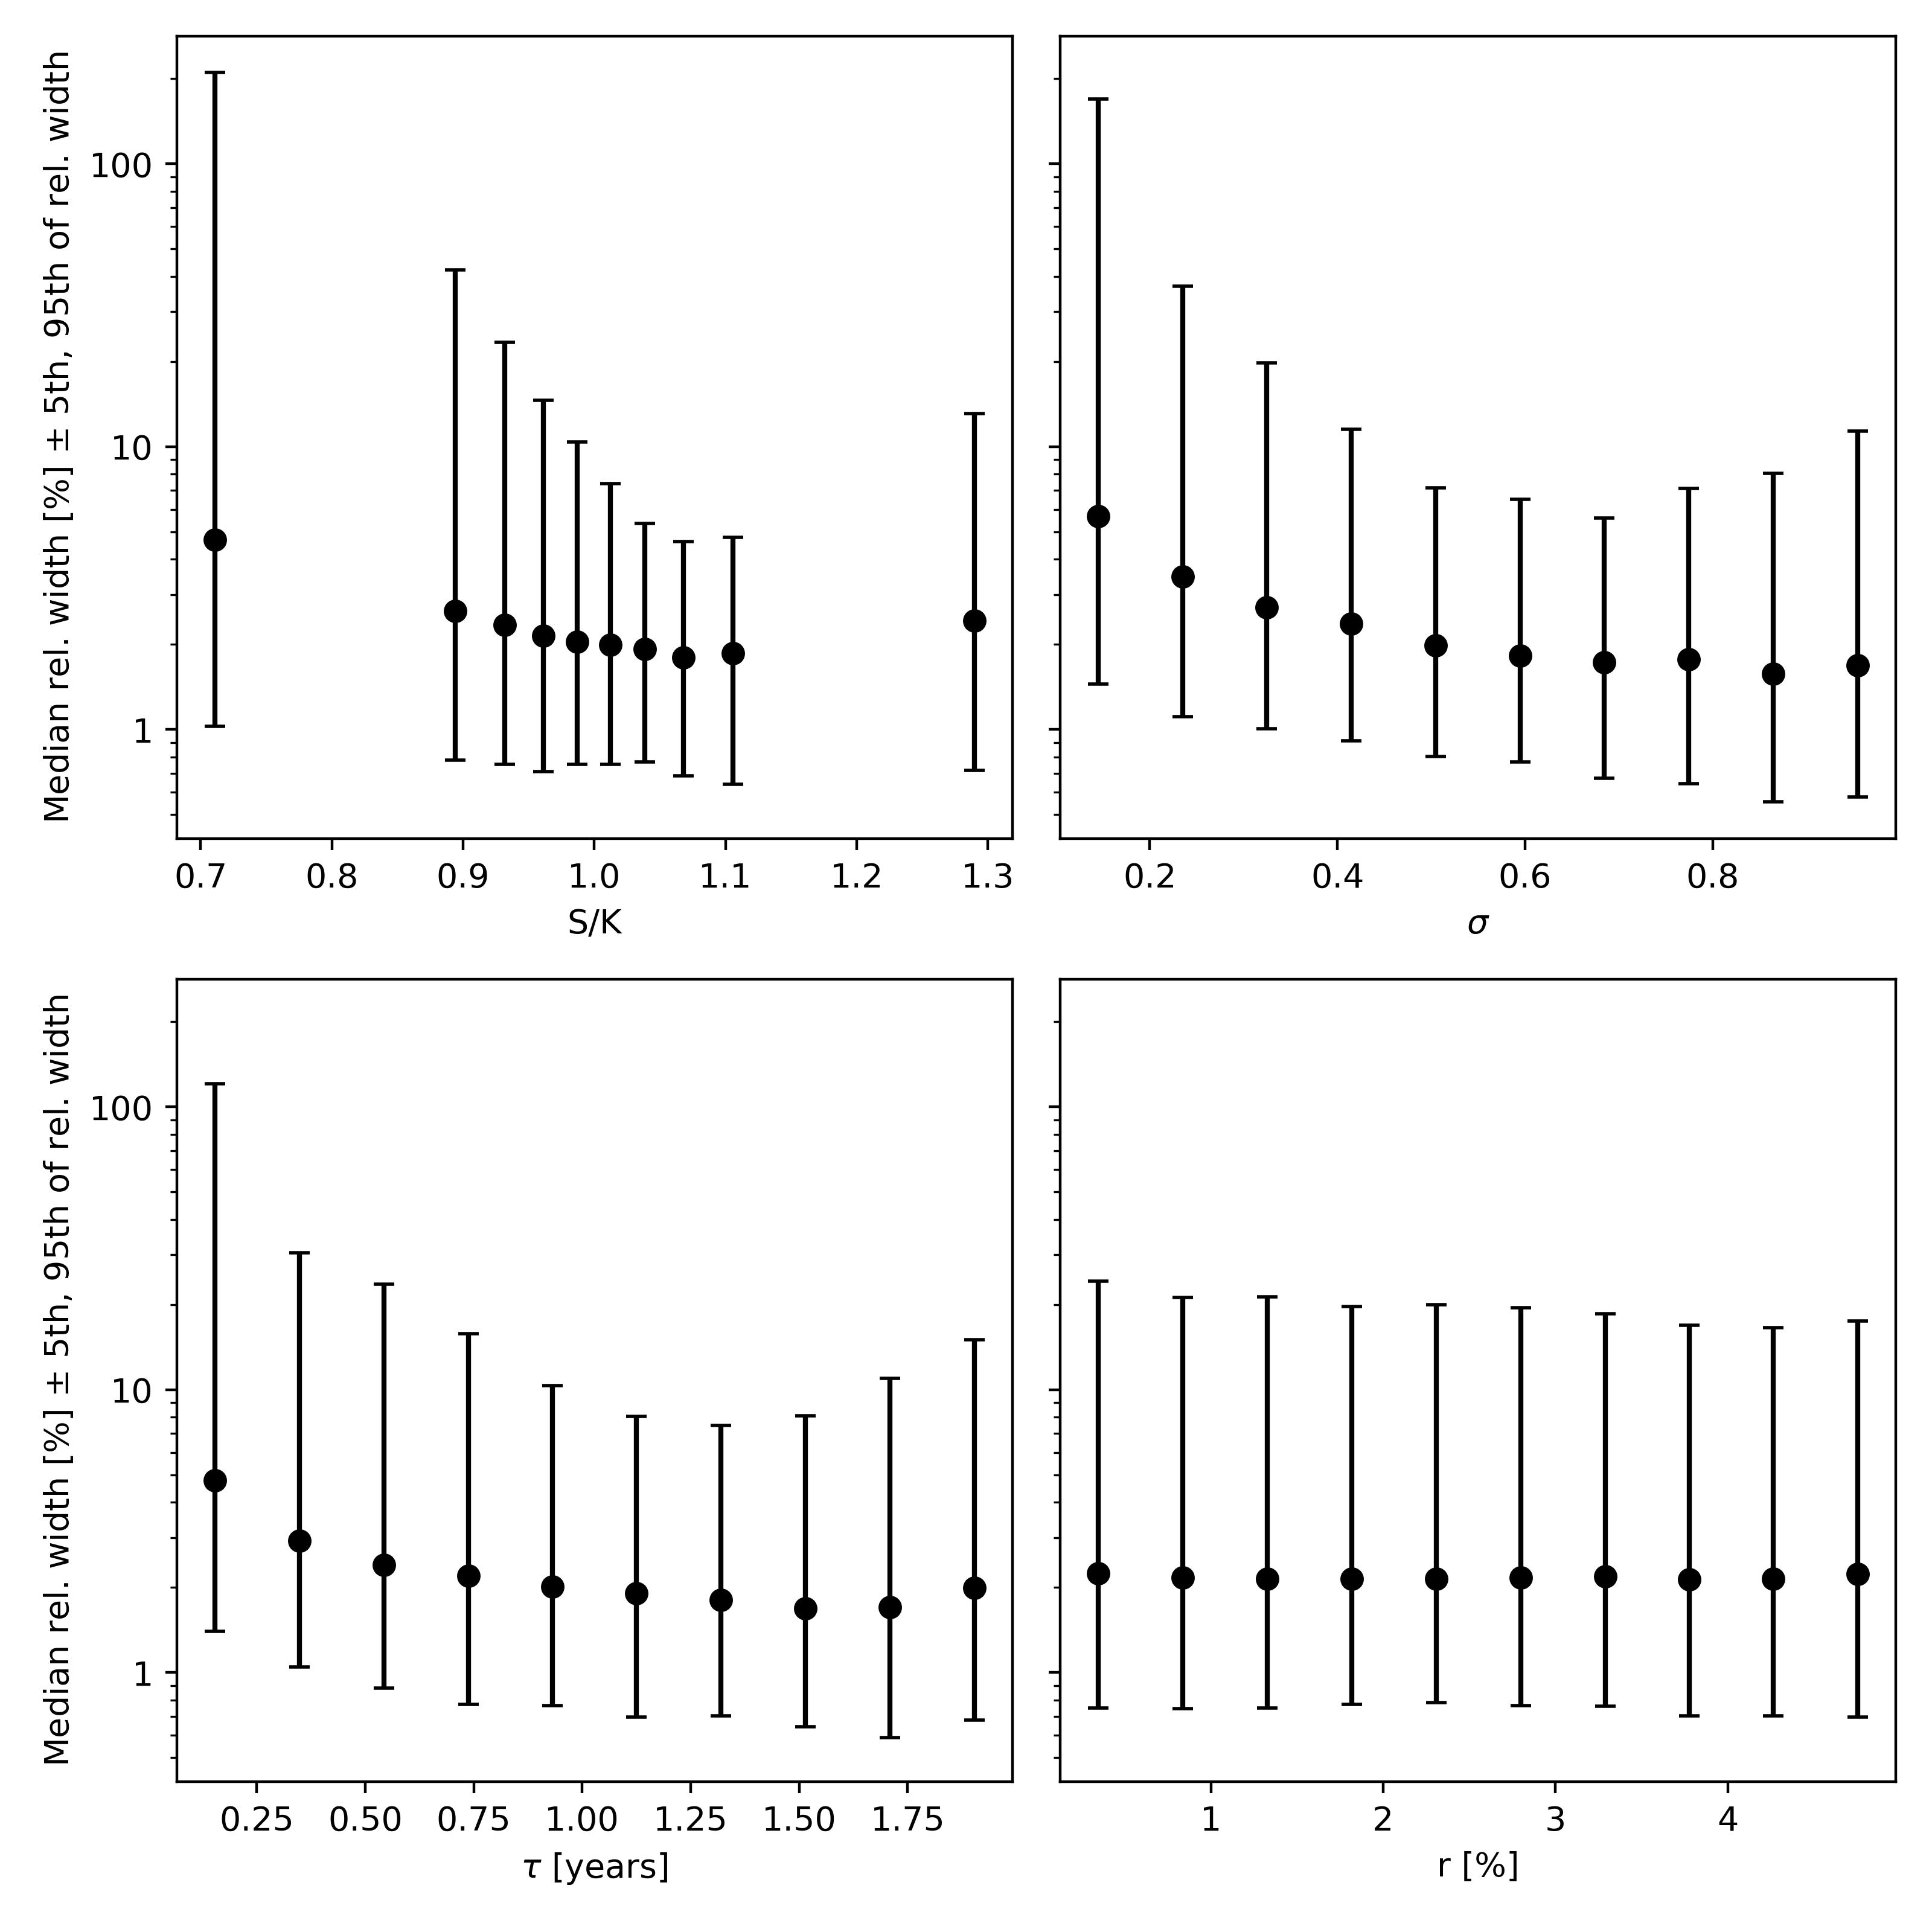
\includegraphics[width=0.8\textwidth]{reports/figures/simulated_data/sim_kappa1_rel_widths_to_features.png}
\caption{Relative widths of PIs accross features for $\kappa=1$.}
\end{figure}

\begin{figure}
\centering
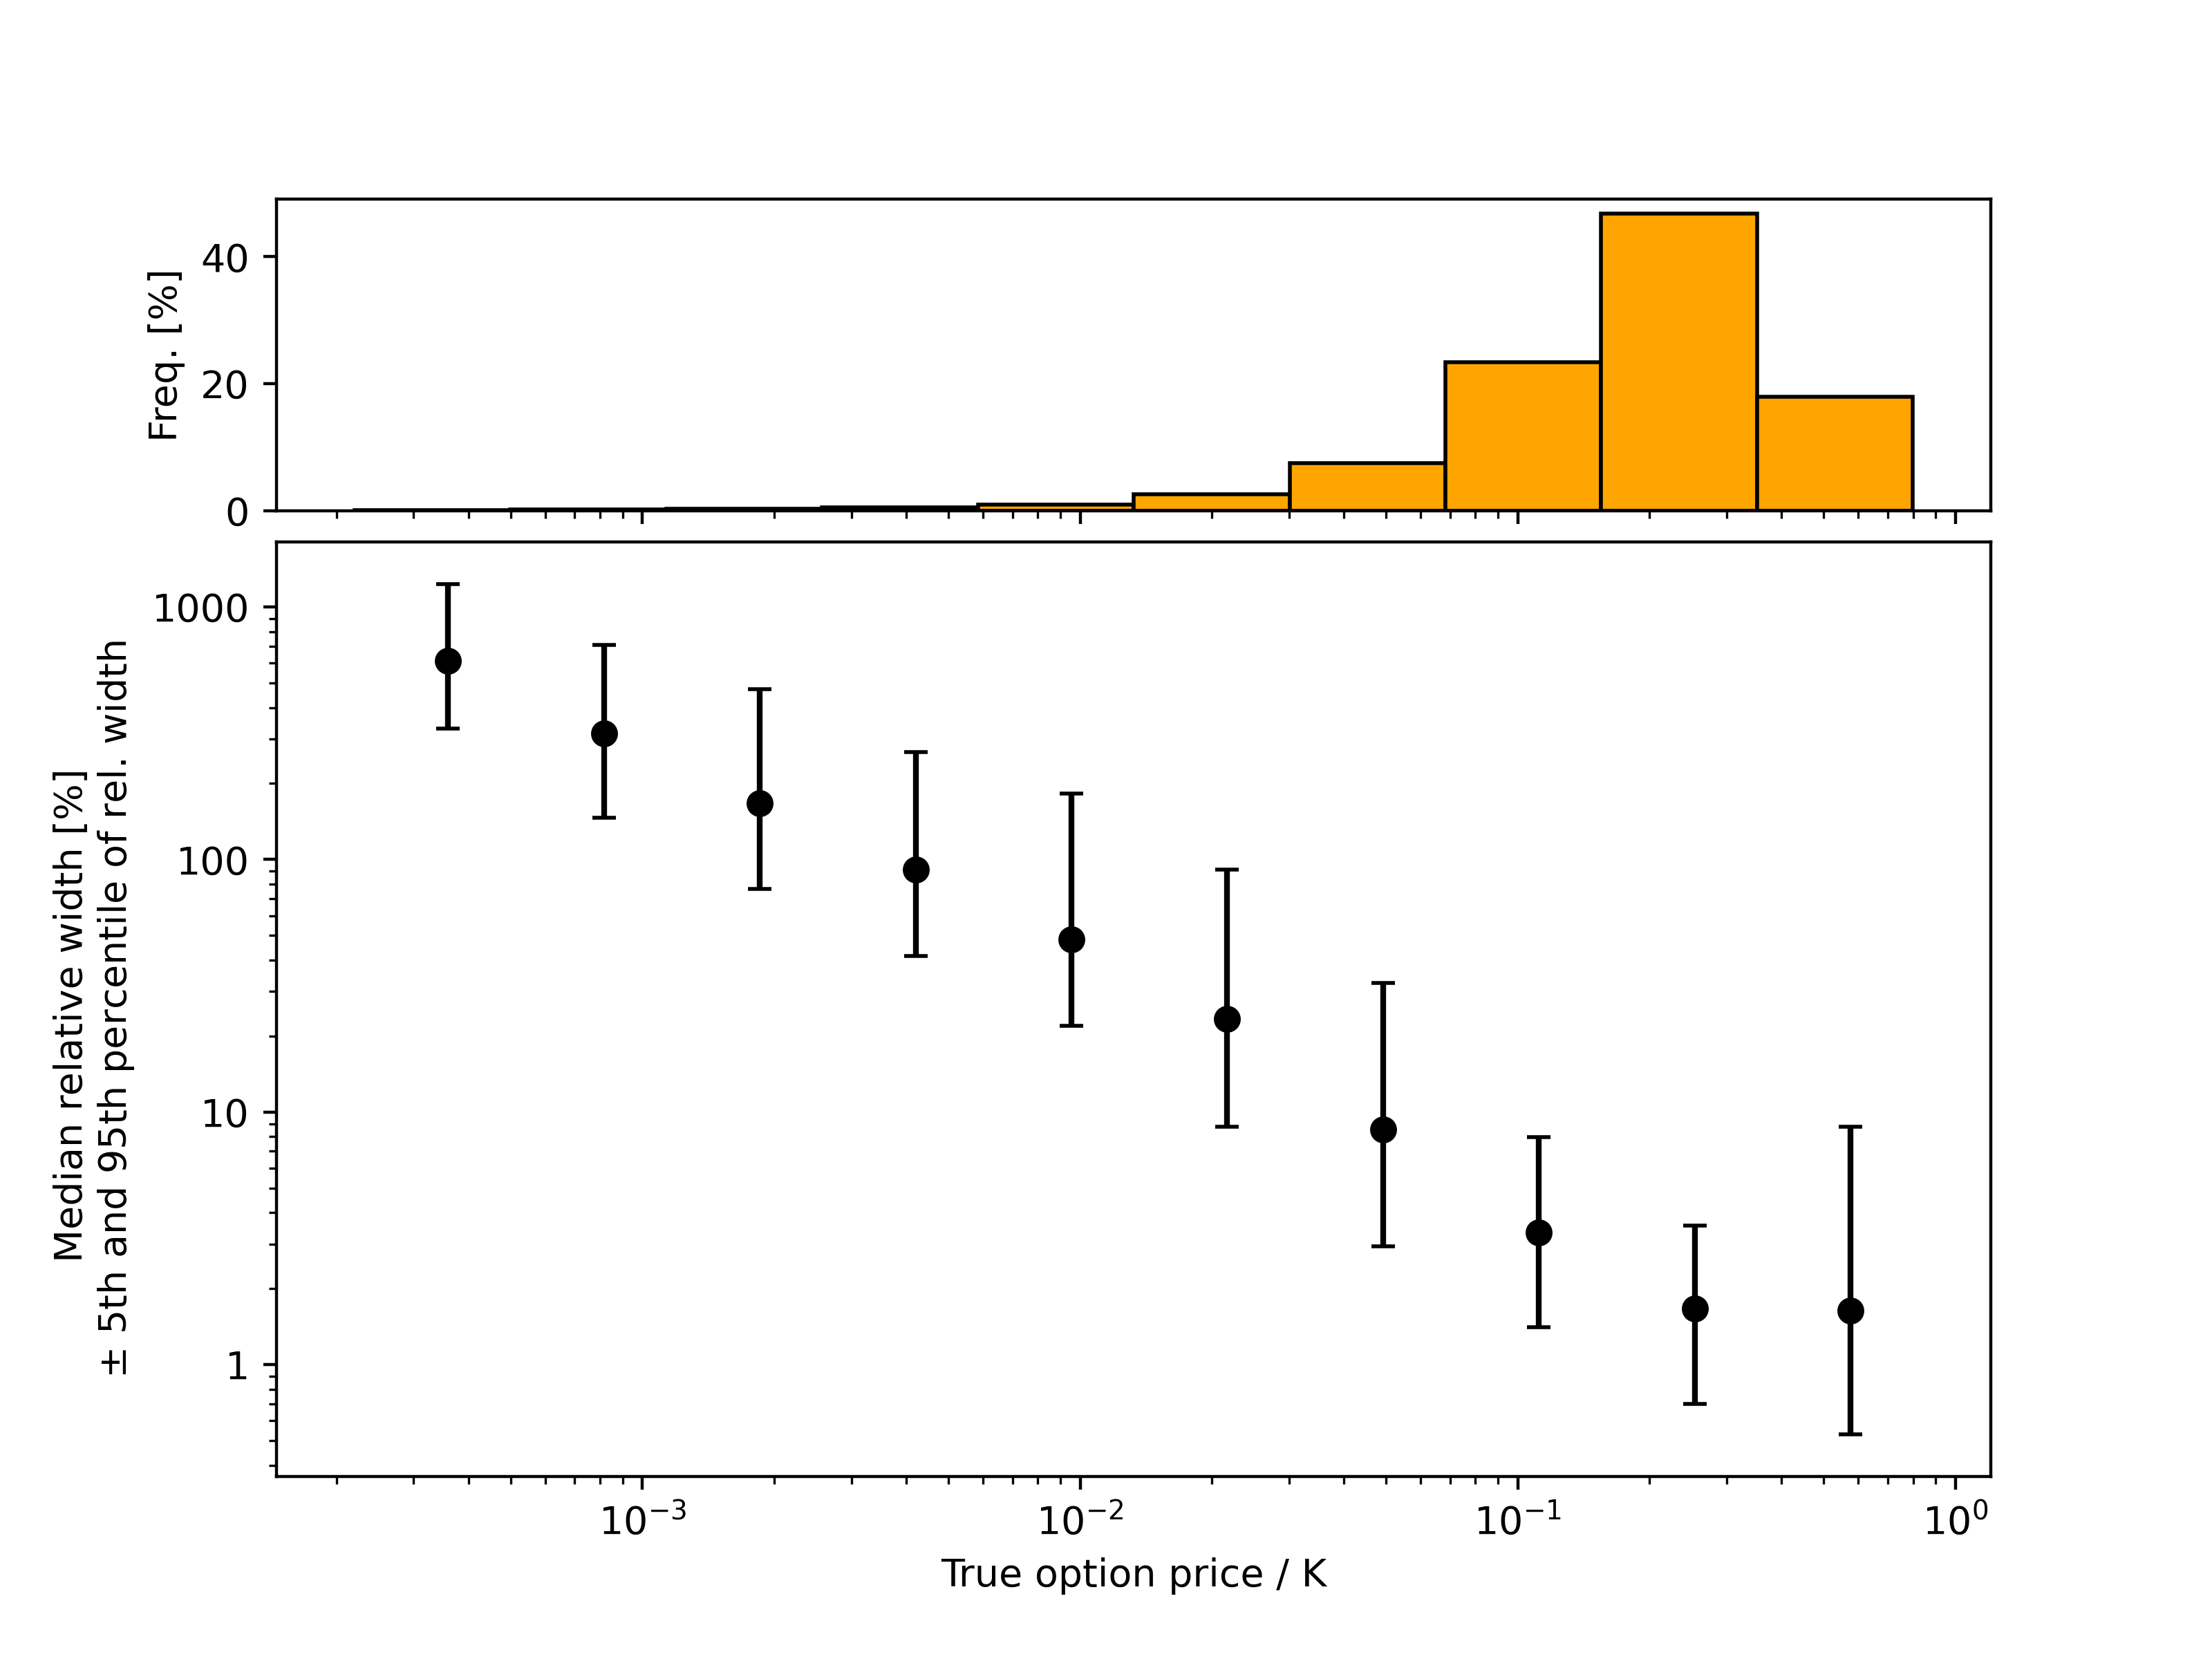
\includegraphics[width=0.8\textwidth]{reports/figures/simulated_data/sim_kappa1_rel_widths_to_opt_price.png}
\caption{PIs binned by the value of the target variable for $\kappa=1$.}
\end{figure}

% kappa = 20

\begin{figure}
\centering
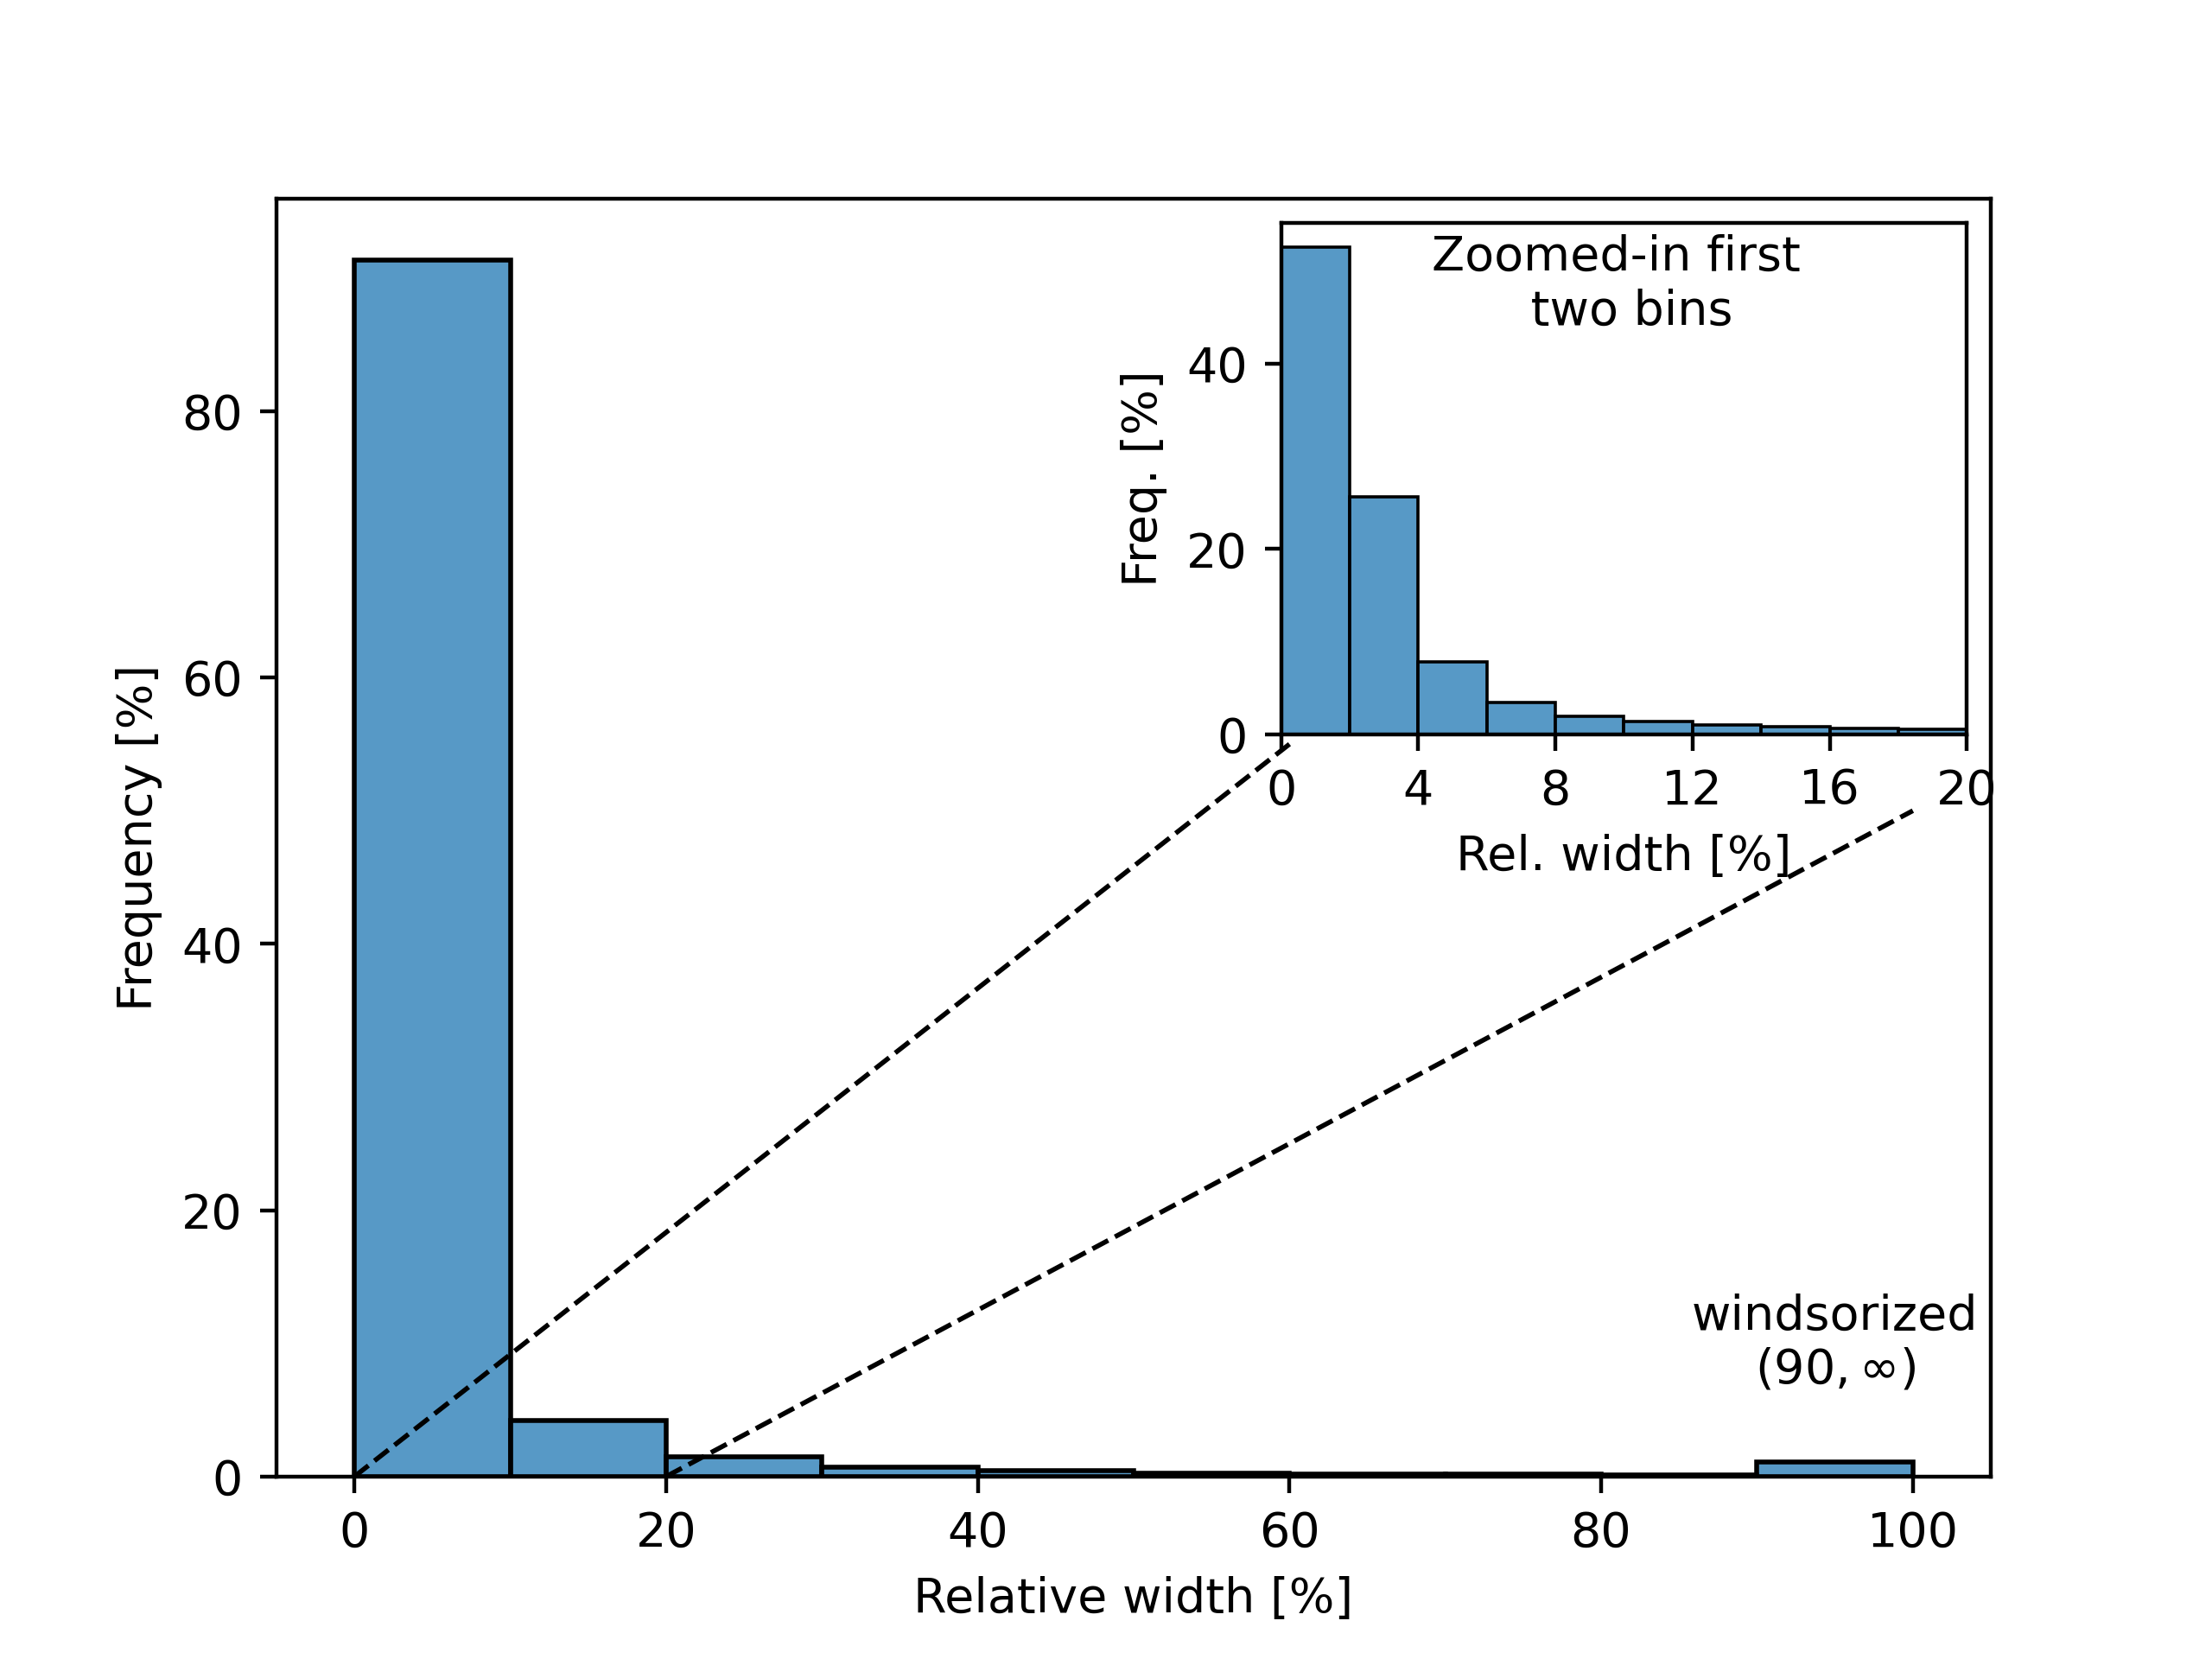
\includegraphics[width=0.8\textwidth]{reports/figures/simulated_data/sim_kappa20_relative_widths.png}
\caption{Distributions of relative widths of PIs for $\kappa=20$.}
%\label{fig:kappa4_rel_widths}
\end{figure}

\begin{figure}
\centering
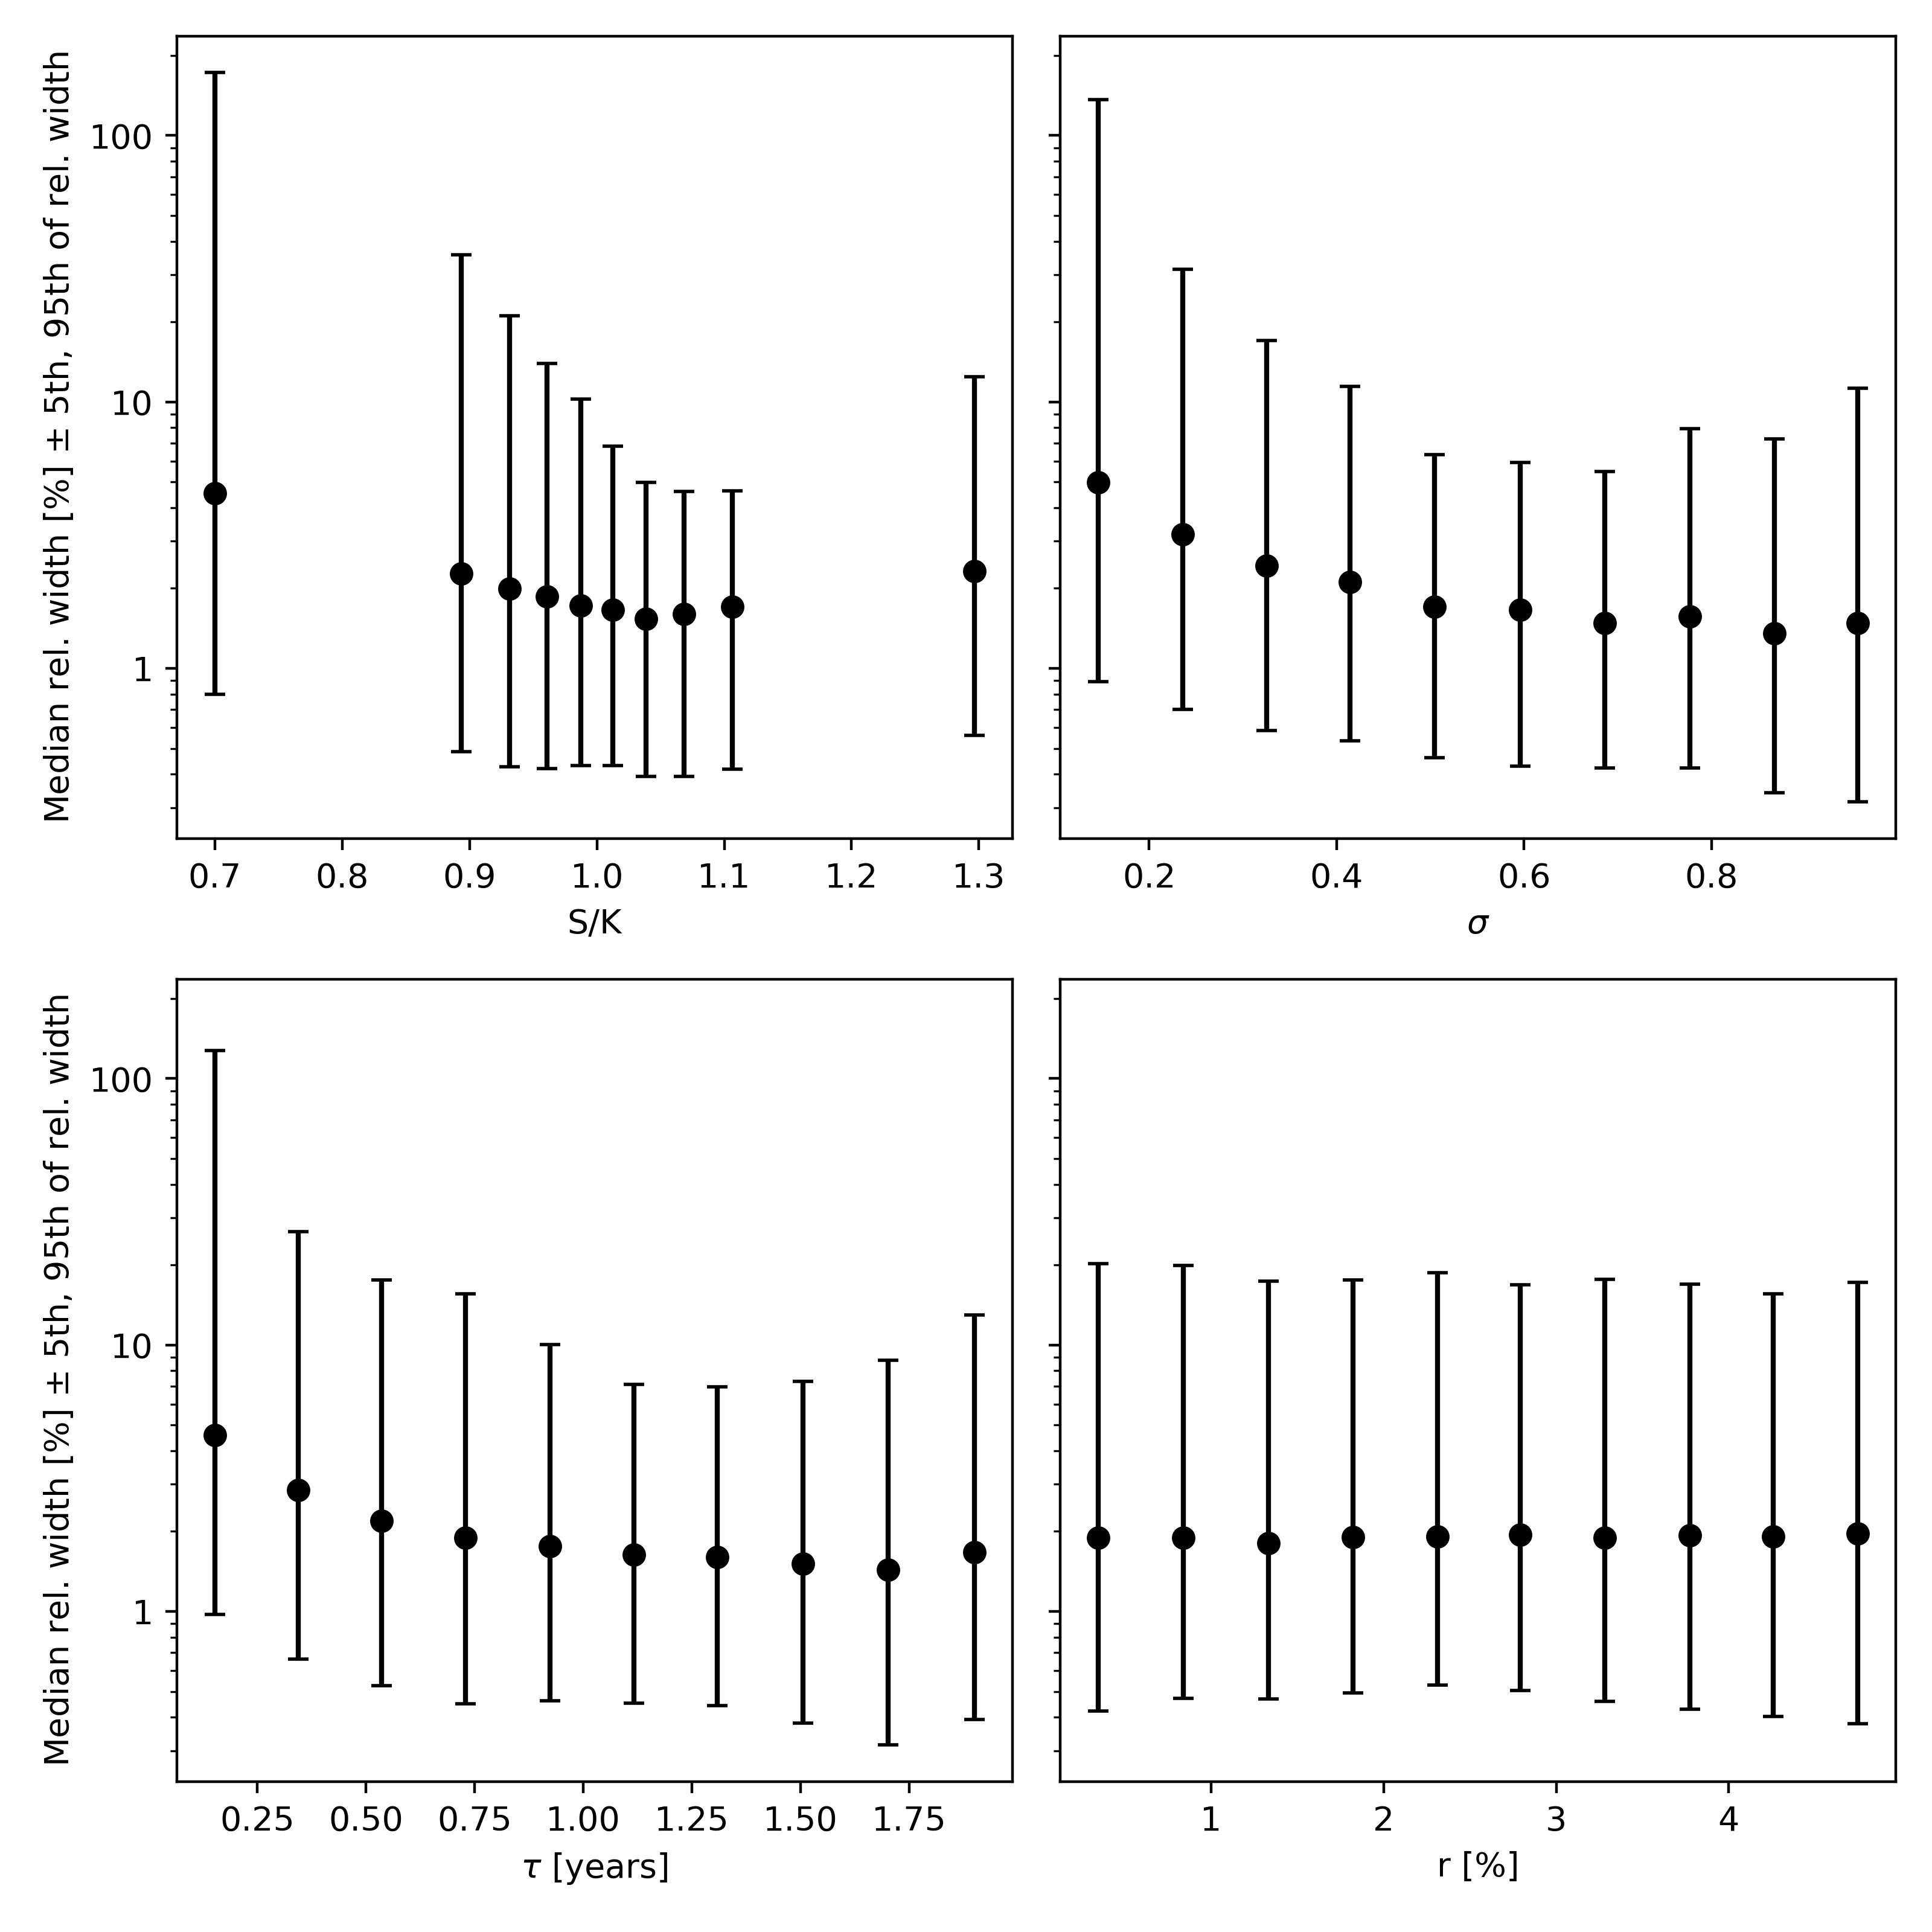
\includegraphics[width=0.8\textwidth]{reports/figures/simulated_data/sim_kappa20_rel_widths_to_features.png}
\caption{Relative widths of PIs accross features for $\kappa=20$.}
\end{figure}

\begin{figure}
\centering
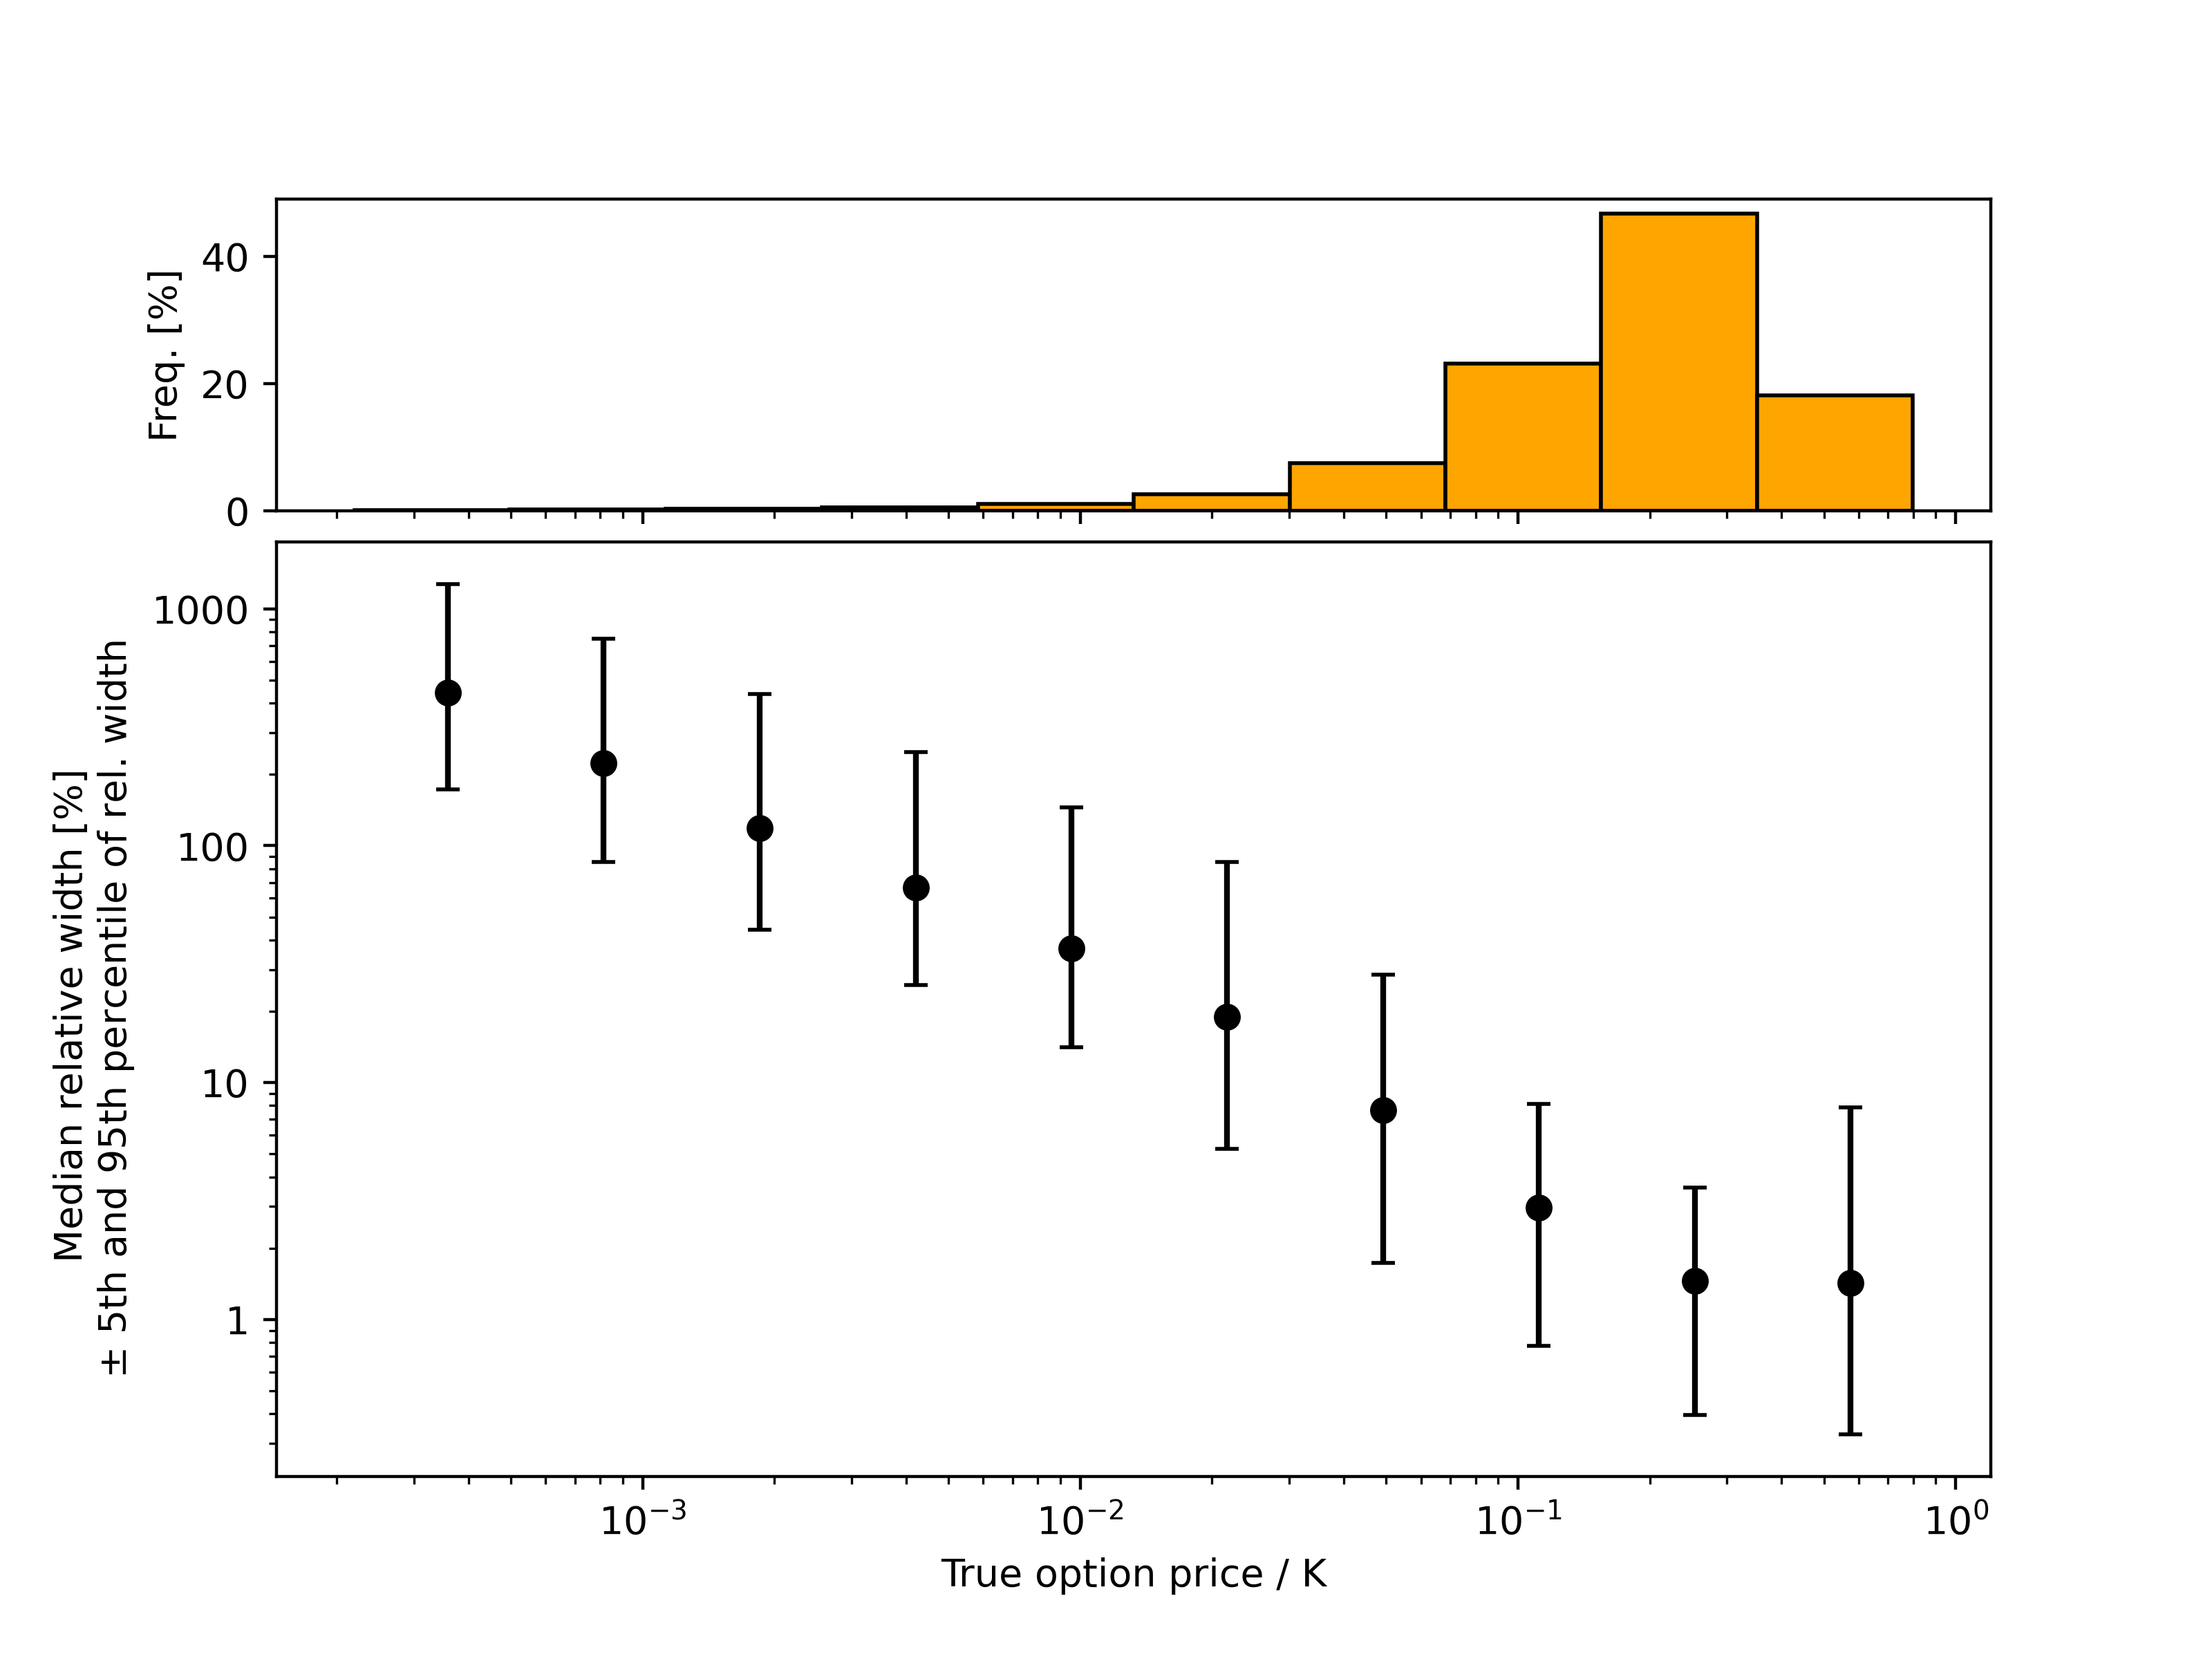
\includegraphics[width=0.8\textwidth]{reports/figures/simulated_data/sim_kappa20_rel_widths_to_opt_price.png}
\caption{PIs binned by the value of the target variable for $\kappa=20$.}
\end{figure}

%%%%%%%%%%%%%%
%   Real data - replication part

\begin{figure}
\centering
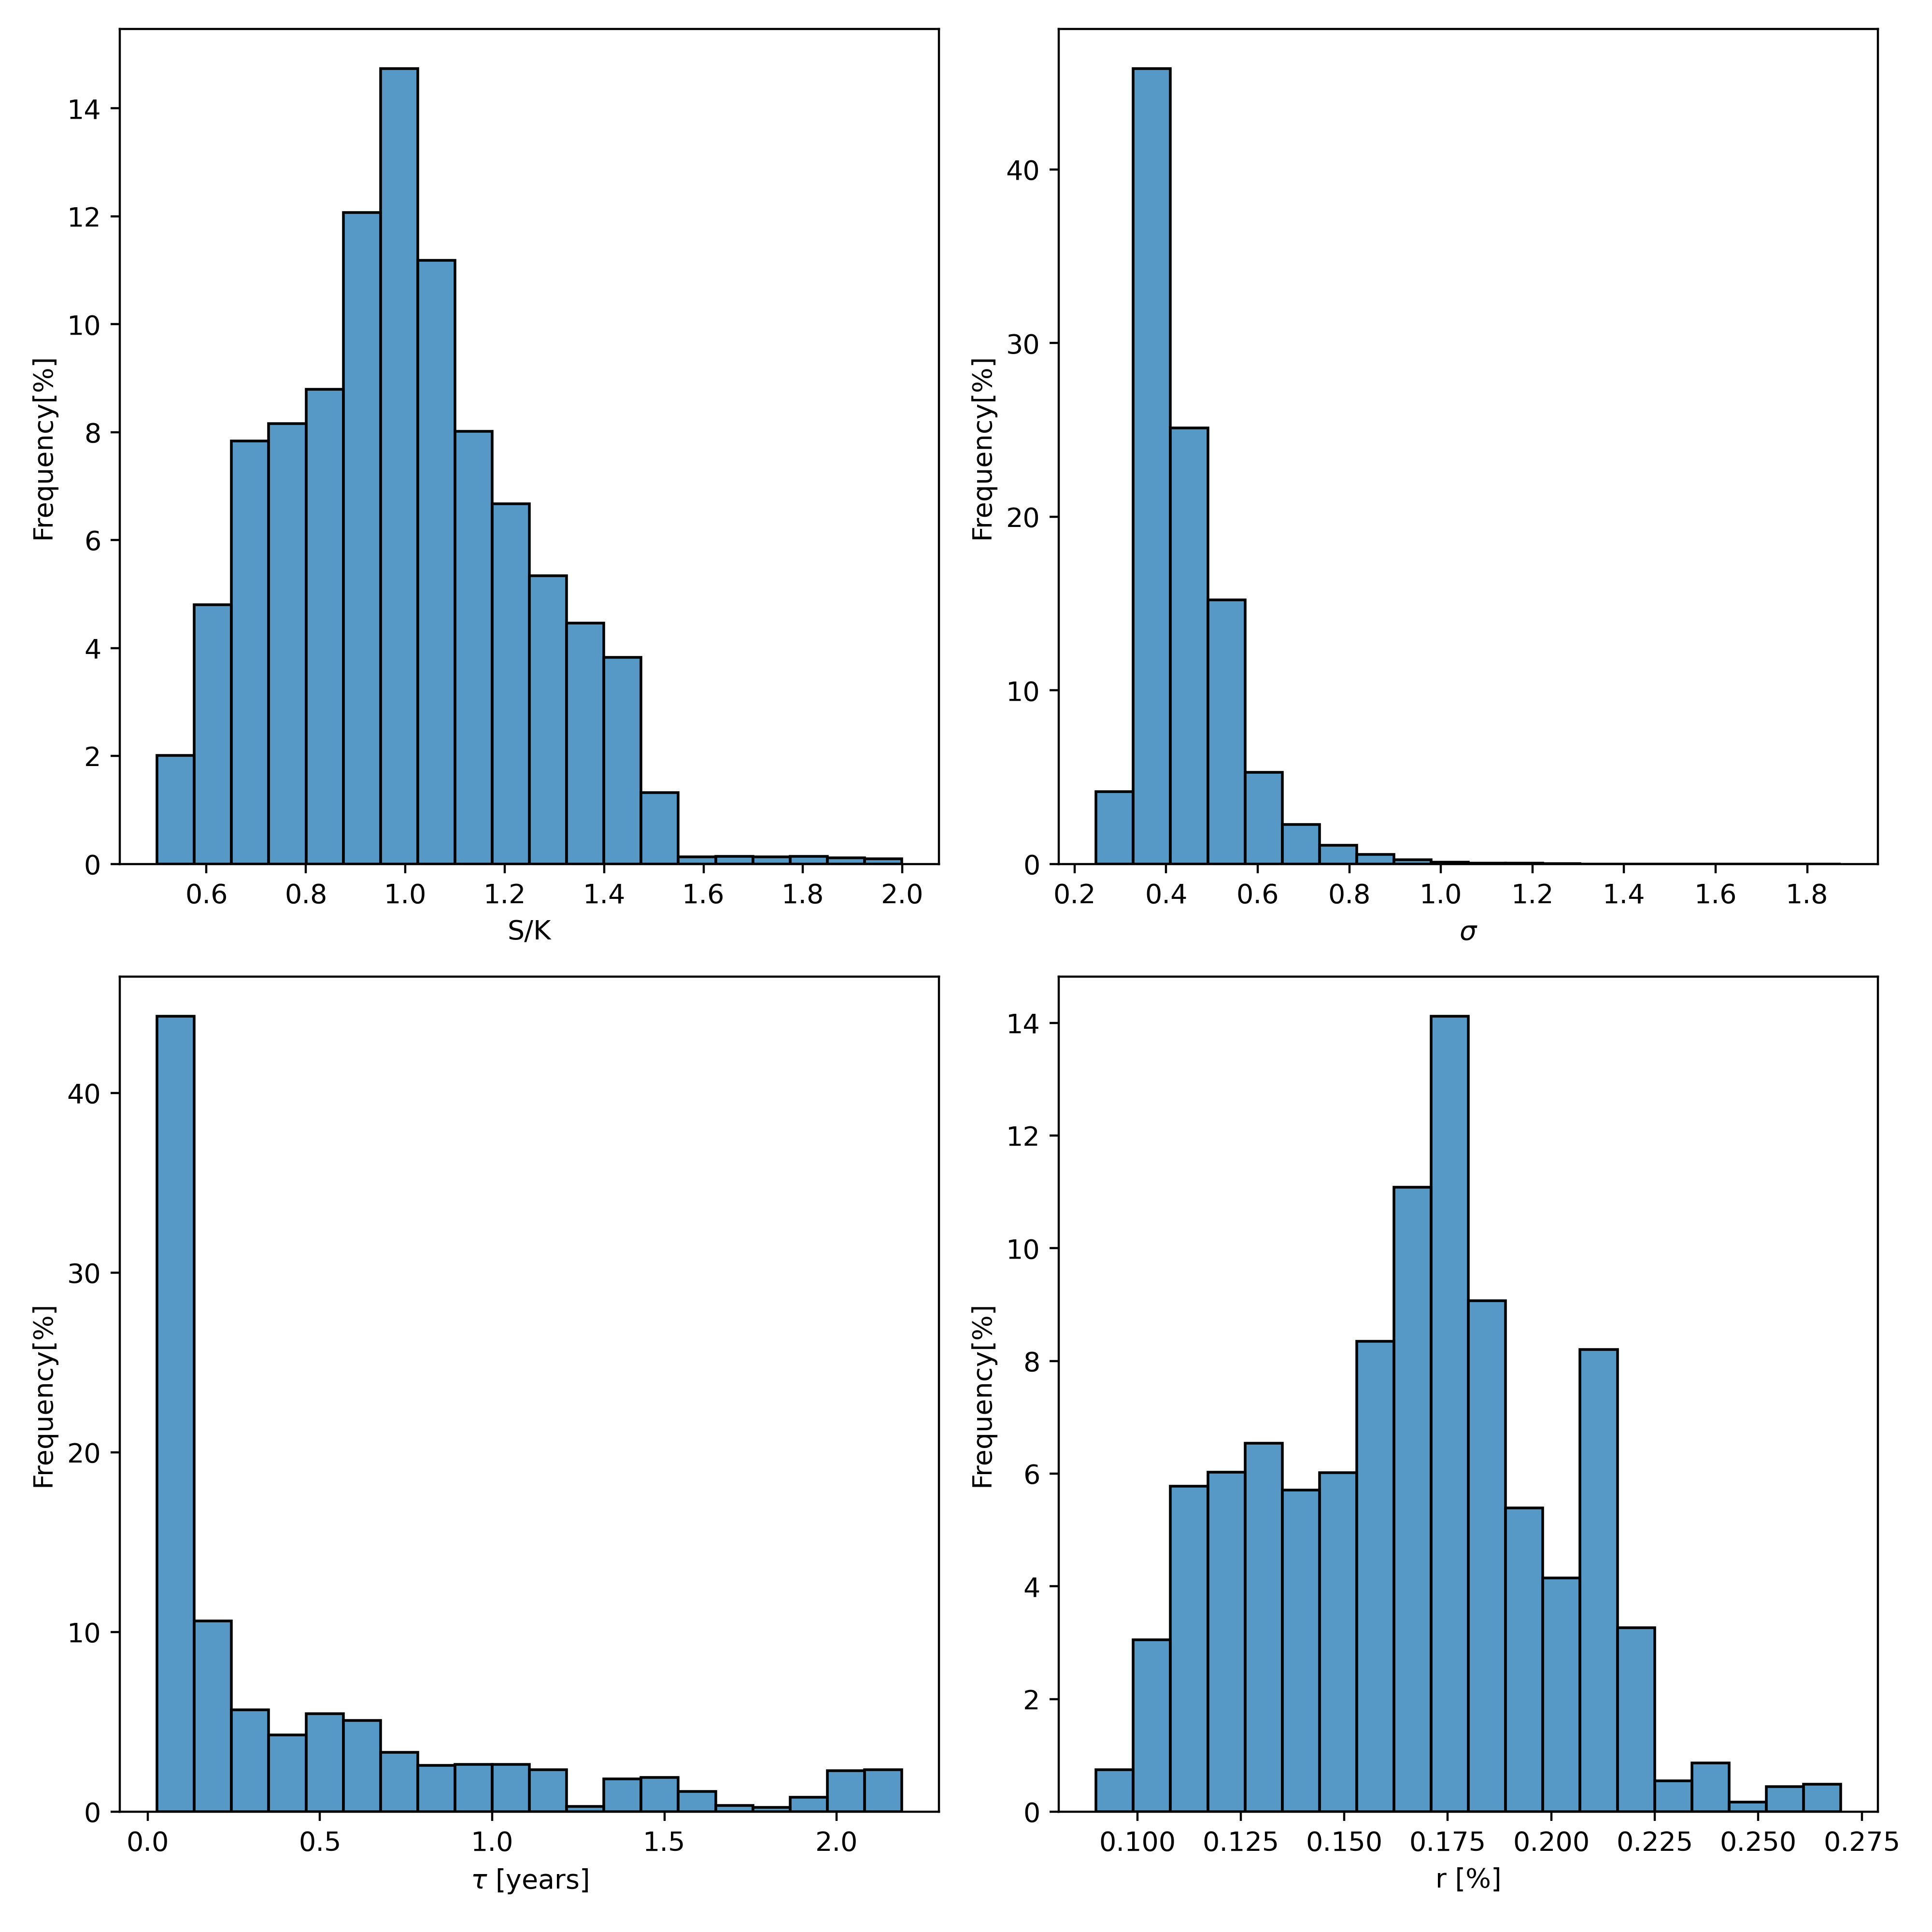
\includegraphics[width=0.9\textwidth]{reports/figures/real_data_replication/real1_feature_distributions.png}
\caption{Relative widths of PIs across features.}
\label{fig:real1_features_dist}
\end{figure}






\end{document}


